% Options for packages loaded elsewhere
\PassOptionsToPackage{unicode}{hyperref}
\PassOptionsToPackage{hyphens}{url}
\PassOptionsToPackage{dvipsnames,svgnames,x11names}{xcolor}
%
\documentclass[
  letterpaper,
  DIV=11,
  numbers=noendperiod]{scrreprt}

\usepackage{amsmath,amssymb}
\usepackage{iftex}
\ifPDFTeX
  \usepackage[T1]{fontenc}
  \usepackage[utf8]{inputenc}
  \usepackage{textcomp} % provide euro and other symbols
\else % if luatex or xetex
  \usepackage{unicode-math}
  \defaultfontfeatures{Scale=MatchLowercase}
  \defaultfontfeatures[\rmfamily]{Ligatures=TeX,Scale=1}
\fi
\usepackage{lmodern}
\ifPDFTeX\else  
    % xetex/luatex font selection
\fi
% Use upquote if available, for straight quotes in verbatim environments
\IfFileExists{upquote.sty}{\usepackage{upquote}}{}
\IfFileExists{microtype.sty}{% use microtype if available
  \usepackage[]{microtype}
  \UseMicrotypeSet[protrusion]{basicmath} % disable protrusion for tt fonts
}{}
\makeatletter
\@ifundefined{KOMAClassName}{% if non-KOMA class
  \IfFileExists{parskip.sty}{%
    \usepackage{parskip}
  }{% else
    \setlength{\parindent}{0pt}
    \setlength{\parskip}{6pt plus 2pt minus 1pt}}
}{% if KOMA class
  \KOMAoptions{parskip=half}}
\makeatother
\usepackage{xcolor}
\setlength{\emergencystretch}{3em} % prevent overfull lines
\setcounter{secnumdepth}{1}
% Make \paragraph and \subparagraph free-standing
\ifx\paragraph\undefined\else
  \let\oldparagraph\paragraph
  \renewcommand{\paragraph}[1]{\oldparagraph{#1}\mbox{}}
\fi
\ifx\subparagraph\undefined\else
  \let\oldsubparagraph\subparagraph
  \renewcommand{\subparagraph}[1]{\oldsubparagraph{#1}\mbox{}}
\fi


\providecommand{\tightlist}{%
  \setlength{\itemsep}{0pt}\setlength{\parskip}{0pt}}\usepackage{longtable,booktabs,array}
\usepackage{calc} % for calculating minipage widths
% Correct order of tables after \paragraph or \subparagraph
\usepackage{etoolbox}
\makeatletter
\patchcmd\longtable{\par}{\if@noskipsec\mbox{}\fi\par}{}{}
\makeatother
% Allow footnotes in longtable head/foot
\IfFileExists{footnotehyper.sty}{\usepackage{footnotehyper}}{\usepackage{footnote}}
\makesavenoteenv{longtable}
\usepackage{graphicx}
\makeatletter
\def\maxwidth{\ifdim\Gin@nat@width>\linewidth\linewidth\else\Gin@nat@width\fi}
\def\maxheight{\ifdim\Gin@nat@height>\textheight\textheight\else\Gin@nat@height\fi}
\makeatother
% Scale images if necessary, so that they will not overflow the page
% margins by default, and it is still possible to overwrite the defaults
% using explicit options in \includegraphics[width, height, ...]{}
\setkeys{Gin}{width=\maxwidth,height=\maxheight,keepaspectratio}
% Set default figure placement to htbp
\makeatletter
\def\fps@figure{htbp}
\makeatother
\newlength{\cslhangindent}
\setlength{\cslhangindent}{1.5em}
\newlength{\csllabelwidth}
\setlength{\csllabelwidth}{3em}
\newlength{\cslentryspacingunit} % times entry-spacing
\setlength{\cslentryspacingunit}{\parskip}
\newenvironment{CSLReferences}[2] % #1 hanging-ident, #2 entry spacing
 {% don't indent paragraphs
  \setlength{\parindent}{0pt}
  % turn on hanging indent if param 1 is 1
  \ifodd #1
  \let\oldpar\par
  \def\par{\hangindent=\cslhangindent\oldpar}
  \fi
  % set entry spacing
  \setlength{\parskip}{#2\cslentryspacingunit}
 }%
 {}
\usepackage{calc}
\newcommand{\CSLBlock}[1]{#1\hfill\break}
\newcommand{\CSLLeftMargin}[1]{\parbox[t]{\csllabelwidth}{#1}}
\newcommand{\CSLRightInline}[1]{\parbox[t]{\linewidth - \csllabelwidth}{#1}\break}
\newcommand{\CSLIndent}[1]{\hspace{\cslhangindent}#1}

\usepackage{makeidx}
\makeindex
\KOMAoption{captions}{tableheading}
\makeatletter
\@ifpackageloaded{tcolorbox}{}{\usepackage[skins,breakable]{tcolorbox}}
\@ifpackageloaded{fontawesome5}{}{\usepackage{fontawesome5}}
\definecolor{quarto-callout-color}{HTML}{909090}
\definecolor{quarto-callout-note-color}{HTML}{0758E5}
\definecolor{quarto-callout-important-color}{HTML}{CC1914}
\definecolor{quarto-callout-warning-color}{HTML}{EB9113}
\definecolor{quarto-callout-tip-color}{HTML}{00A047}
\definecolor{quarto-callout-caution-color}{HTML}{FC5300}
\definecolor{quarto-callout-color-frame}{HTML}{acacac}
\definecolor{quarto-callout-note-color-frame}{HTML}{4582ec}
\definecolor{quarto-callout-important-color-frame}{HTML}{d9534f}
\definecolor{quarto-callout-warning-color-frame}{HTML}{f0ad4e}
\definecolor{quarto-callout-tip-color-frame}{HTML}{02b875}
\definecolor{quarto-callout-caution-color-frame}{HTML}{fd7e14}
\makeatother
\makeatletter
\makeatother
\makeatletter
\@ifpackageloaded{bookmark}{}{\usepackage{bookmark}}
\makeatother
\makeatletter
\@ifpackageloaded{caption}{}{\usepackage{caption}}
\AtBeginDocument{%
\ifdefined\contentsname
  \renewcommand*\contentsname{Içindekiler}
\else
  \newcommand\contentsname{Içindekiler}
\fi
\ifdefined\listfigurename
  \renewcommand*\listfigurename{Şekil Listesi}
\else
  \newcommand\listfigurename{Şekil Listesi}
\fi
\ifdefined\listtablename
  \renewcommand*\listtablename{Tablo Listesi}
\else
  \newcommand\listtablename{Tablo Listesi}
\fi
\ifdefined\figurename
  \renewcommand*\figurename{Figür}
\else
  \newcommand\figurename{Figür}
\fi
\ifdefined\tablename
  \renewcommand*\tablename{Tablo}
\else
  \newcommand\tablename{Tablo}
\fi
}
\@ifpackageloaded{float}{}{\usepackage{float}}
\floatstyle{ruled}
\@ifundefined{c@chapter}{\newfloat{codelisting}{h}{lop}}{\newfloat{codelisting}{h}{lop}[chapter]}
\floatname{codelisting}{Listeleme}
\newcommand*\listoflistings{\listof{codelisting}{İlan Listesi}}
\makeatother
\makeatletter
\@ifpackageloaded{caption}{}{\usepackage{caption}}
\@ifpackageloaded{subcaption}{}{\usepackage{subcaption}}
\makeatother
\makeatletter
\@ifpackageloaded{tcolorbox}{}{\usepackage[skins,breakable]{tcolorbox}}
\makeatother
\makeatletter
\@ifundefined{shadecolor}{\definecolor{shadecolor}{rgb}{.97, .97, .97}}
\makeatother
\makeatletter
\makeatother
\makeatletter
\makeatother
\ifLuaTeX
\usepackage[bidi=basic]{babel}
\else
\usepackage[bidi=default]{babel}
\fi
\babelprovide[main,import]{turkish}
% get rid of language-specific shorthands (see #6817):
\let\LanguageShortHands\languageshorthands
\def\languageshorthands#1{}
\ifLuaTeX
  \usepackage{selnolig}  % disable illegal ligatures
\fi
\IfFileExists{bookmark.sty}{\usepackage{bookmark}}{\usepackage{hyperref}}
\IfFileExists{xurl.sty}{\usepackage{xurl}}{} % add URL line breaks if available
\urlstyle{same} % disable monospaced font for URLs
\hypersetup{
  pdftitle={Patoloji Atlası},
  pdfauthor={Serdar Balcı; Patoloji Hekim ve Teknikerleri},
  pdflang={tr},
  colorlinks=true,
  linkcolor={blue},
  filecolor={Maroon},
  citecolor={Blue},
  urlcolor={Blue},
  pdfcreator={LaTeX via pandoc}}

\title{Patoloji Atlası}
\usepackage{etoolbox}
\makeatletter
\providecommand{\subtitle}[1]{% add subtitle to \maketitle
  \apptocmd{\@title}{\par {\large #1 \par}}{}{}
}
\makeatother
\subtitle{Patoloji Atlası: Tıp Fakültesi ve Sağlık Bilimleri Öğrencileri
İçin Patoloji Laboratuvar Notları: Görerek Öğrenin}
\author{Serdar Balcı \and Patoloji Hekim ve Teknikerleri}
\date{last-modified}

\begin{document}
\maketitle
\begin{abstract}
Patoloji Atlası: Tıp Fakültesi ve Sağlık Bilimleri Öğrencileri İçin
Patoloji Laboratuvar Notları. Görerek Öğrenin. Patoloji Atlası Memorial
Patoloji arşivinden derlenen vakalardan ve diğer kurumlardan katkı yapan
meslektaşlarımızın kolleksiyonlarından oluşmaktadır. Katkı yapmak ve
kendi vakalarınız ekletmek için lütfen
\href{https://www.patolojiatlasi.com/katki.html}{iletişime geçin}.
\end{abstract}
\ifdefined\Shaded\renewenvironment{Shaded}{\begin{tcolorbox}[sharp corners, boxrule=0pt, borderline west={3pt}{0pt}{shadecolor}, interior hidden, breakable, frame hidden, enhanced]}{\end{tcolorbox}}\fi

\renewcommand*\contentsname{İçindekiler}
{
\hypersetup{linkcolor=}
\setcounter{tocdepth}{1}
\tableofcontents
}
\bookmarksetup{startatroot}

\hypertarget{sec-patoloji-atlasi}{%
\chapter*{Patoloji Atlası}\label{sec-patoloji-atlasi}}
\addcontentsline{toc}{chapter}{Patoloji Atlası}

\markboth{Patoloji Atlası}{Patoloji Atlası}

\begin{itemize}
\item
  For English \href{https://www.histopathologyatlas.com/}{click here}.
\item
  Sosyal medyadan derlenen görüntülerden oluşan patoloji notları için
  \href{https://www.patolojinotlari.com/}{tıklayınız}.\\
\end{itemize}

\bookmarksetup{startatroot}

\hypertarget{sec-giris}{%
\chapter*{Giriş}\label{sec-giris}}
\addcontentsline{toc}{chapter}{Giriş}

\markboth{Giriş}{Giriş}

Patoloji Atlası Memorial Patoloji arşivinden ve diğer kurumlardan katkı
yapan meslektaşlarımızın koleksiyonlarından oluşmaktadır.

\href{https://www.patolojiatlasi.com/katki.html}{Katkı yapmak ve kendi
vakalarınız ekletmek için lütfen iletişime geçin}.

\begin{verbatim}
Son güncelleme zamanı: 2023-08-05 23:28:54
\end{verbatim}

Sosyal medyadan derlenen görüntülerden oluşan
\href{https://www.patolojinotlari.com/}{patoloji notları için
tıklayınız}.

\bookmarksetup{startatroot}

\hypertarget{sec-yazarlar-katkida-bulunanlar}{%
\chapter*{Yazarlar ve Katkıda
Bulunanlar}\label{sec-yazarlar-katkida-bulunanlar}}
\addcontentsline{toc}{chapter}{Yazarlar ve Katkıda Bulunanlar}

\markboth{Yazarlar ve Katkıda Bulunanlar}{Yazarlar ve Katkıda
Bulunanlar}

\hypertarget{sec-derleyen}{%
\section*{Derleyen:}\label{sec-derleyen}}
\addcontentsline{toc}{section}{Derleyen:}

\markright{Derleyen:}

\begin{itemize}
\tightlist
\item
  \href{https://www.serdarbalci.com}{Serdar Balcı}
\end{itemize}

\hypertarget{sec-katkida-bulunanlar}{%
\section*{Katkıda Bulunanlar:}\label{sec-katkida-bulunanlar}}
\addcontentsline{toc}{section}{Katkıda Bulunanlar:}

\markright{Katkıda Bulunanlar:}

\href{https://patoloji.memorial.com.tr/}{\textbf{Memorial Patoloji}}
\textbf{Hekimleri}

\begin{itemize}
\item
  \href{https://www.memorial.com.tr/en/doctors/ilknur-turkmen-1975}{İlknur
  Turkmen}
\item
  \href{https://www.memorial.com.tr/doktorlar/gulen-bulbul-dogusoy}{Gülen
  Bülbül Doğusoy}
\item
  \href{https://www.memorial.com.tr/doktorlar/fatma-aktepe}{Fatma
  Aktepe}
\item
  \href{https://www.memorial.com.tr/doktorlar/turkan-atasever-rezanko}{Türkan
  Atasever Rezanko}
\item
  \href{https://www.memorial.com.tr/doktorlar/pembe-gul-gunes}{Pembe Gül
  Güneş}
\item
  \href{https://www.memorial.com.tr/doktorlar/semsi-yildiz-1}{Şemsi
  Yıldız}
\item
  \href{https://www.memorial.com.tr/doktorlar/serdar-balci-k}{Serdar
  Balcı}
\item
  \href{https://www.memorial.com.tr/doktorlar/sezen-kocarslan}{Sezen
  Koçarslan}
\item
  \href{https://www.memorial.com.tr/doktorlar/yildirim-karslioglu-k}{Yıldırım
  Karslıoğlu}
\item
  \href{https://www.memorial.com.tr/doktorlar/mehtat-uz-unlu-k}{Mehtat
  Uz Ünlü}
\item
  \href{https://www.memorial.com.tr/doktorlar/murat-oktay}{Murat Oktay}
\item
  Deniz Bayçelebi
\item
  \href{https://www.memorial.com.tr/doktorlar/emre-karakok}{Emre
  Karakök}
\item
  Zuhal Kuş Sılav
\item
  \href{https://www.memorial.com.tr/doktorlar/fatma-gulgun-sade-kocak-k}{Fatma
  Gülgün Sade Koçak}
\item
  \href{https://www.memorial.com.tr/doktorlar/zeynep-pehlivanoglu-k}{Zeynep
  Pehlivanoğlu}
\item
  \href{https://www.memorial.com.tr/doktorlar/fadime-gul-salman}{Fadime
  Gül Salman}
\end{itemize}

\href{https://patoloji.memorial.com.tr/}{\textbf{Memorial Patoloji}}
\textbf{Teknikerleri}

\begin{itemize}
\item
  Emrah Uça
\item
  \href{https://www.linkedin.com/in/\%C5\%9Fevin-elif-\%C5\%9Fanio\%C4\%9Flu-99449a1b0/}{Şevin
  Elif Şanioğlu}
\item
  \href{https://www.linkedin.com/in/baset-s\%C4\%B1\%C4\%9F\%C4\%B1rc\%C4\%B1-aa2406141/}{Baset
  Sığırcı}
\item
  \href{https://www.linkedin.com/in/rabia-\%C3\%B6zt\%C3\%BCrk-4989b3151/}{Rabia
  Öztürk}
\item
  Zehra Yaşaroğlu
\item
  Baha Erdoğan
\item
  Talha Akbaş
\end{itemize}

\hypertarget{sec-diger-kurumlardan-katkida-bulunanlar}{%
\section*{Diğer Kurumlardan Katkıda
Bulunanlar}\label{sec-diger-kurumlardan-katkida-bulunanlar}}
\addcontentsline{toc}{section}{Diğer Kurumlardan Katkıda Bulunanlar}

\markright{Diğer Kurumlardan Katkıda Bulunanlar}

\begin{itemize}
\item
  \href{https://github.com/veterinarypathology3d}{Tarık Atmaca}
\item
  \href{https://hacettepepathology.com/}{Kemal Kösemehmetoğlu}
\item
  \href{https://www.hastane.hacettepe.edu.tr/115.html?drid=479}{Arzu
  Sağlam Ayhan}
\item
  \href{https://scholar.google.com.tr/citations?user=9e7r9yQAAAAJ}{Burcu
  Saka}
\item
  \href{https://www.florence.com.tr/prof-dr-ipek-coban-elbegi}{İpek
  Çoban Elbeği}
\end{itemize}

\part{Genel Patoloji}

\hypertarget{sec-patolojide-kullanilan-teknikler}{%
\chapter{Patolojide Kullanılan
Teknikler}\label{sec-patolojide-kullanilan-teknikler}}

\hypertarget{sec-histokimya}{%
\section{Histokimya}\label{sec-histokimya}}

\hypertarget{sec-musin}{%
\subsection{Müsin}\label{sec-musin}}

\hypertarget{sec-mucicarmine}{%
\subsubsection{Mucicarmine}\label{sec-mucicarmine}}

\textbf{Normal kolon mukozasında intrasitoplazmik müsini gösteren
mucicarmine (müsikarmen) histokimyası}


\includegraphics[width=0.15\textwidth,height=\textheight]{index_files/mediabag/qrcodes/mucicarmine_qrcode.pdf}
\href{https://images.patolojiatlasi.com/mucin/mucicarmine.html}{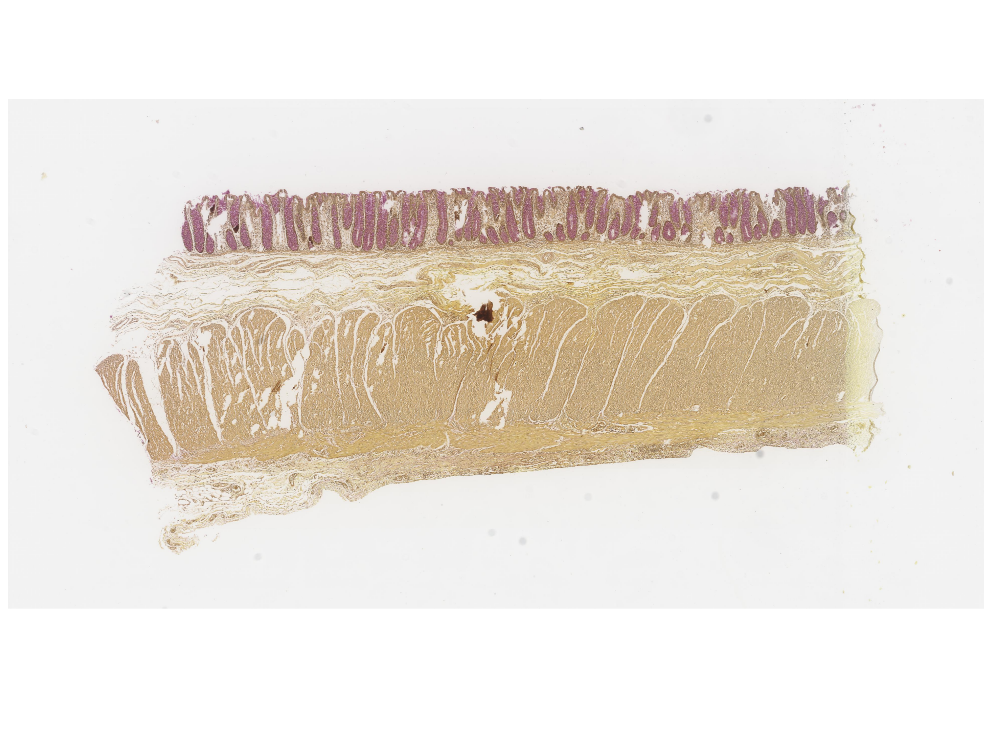
\includegraphics[width=0.25\textwidth,height=\textheight]{./screenshots/thumbnail_mucicarmine.png}}
\href{https://images.patolojiatlasi.com/mucin/mucicarmine.html}{Tam
Ekran Görmek İçin Resmi Tıklayın}

\hypertarget{sec-chromogenic-in-situ-hybridization-cish}{%
\section{Chromogenic in situ hybridization
(CISH)}\label{sec-chromogenic-in-situ-hybridization-cish}}

\textbf{Chromogenic in situ hybridization (CISH)}

\href{https://images.patolojiatlasi.com/her2-cish/cish.html}{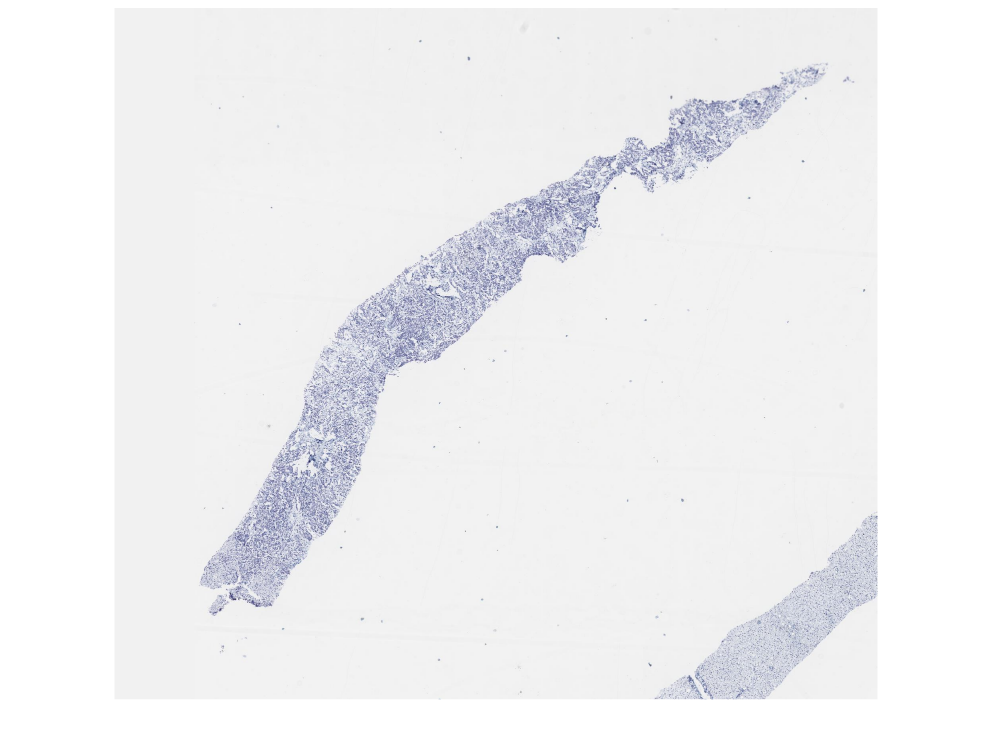
\includegraphics[width=0.25\textwidth,height=\textheight]{./screenshots/thumbnail_cish.png}}
\href{https://images.patolojiatlasi.com/her2-cish/cish.html}{Tam Ekran
Görmek İçin Resmi Tıklayın}

\hypertarget{sec-hucre-ici-birikimler}{%
\chapter{Hücre İçi Birikimler}\label{sec-hucre-ici-birikimler}}

\hypertarget{sec-kolesterol-polibi}{%
\section{Kolesterol Polibi}\label{sec-kolesterol-polibi}}

\textbf{Kolesterol Polibi}

\href{https://images.patolojiatlasi.com/cholesterolpolyp/HE.html}{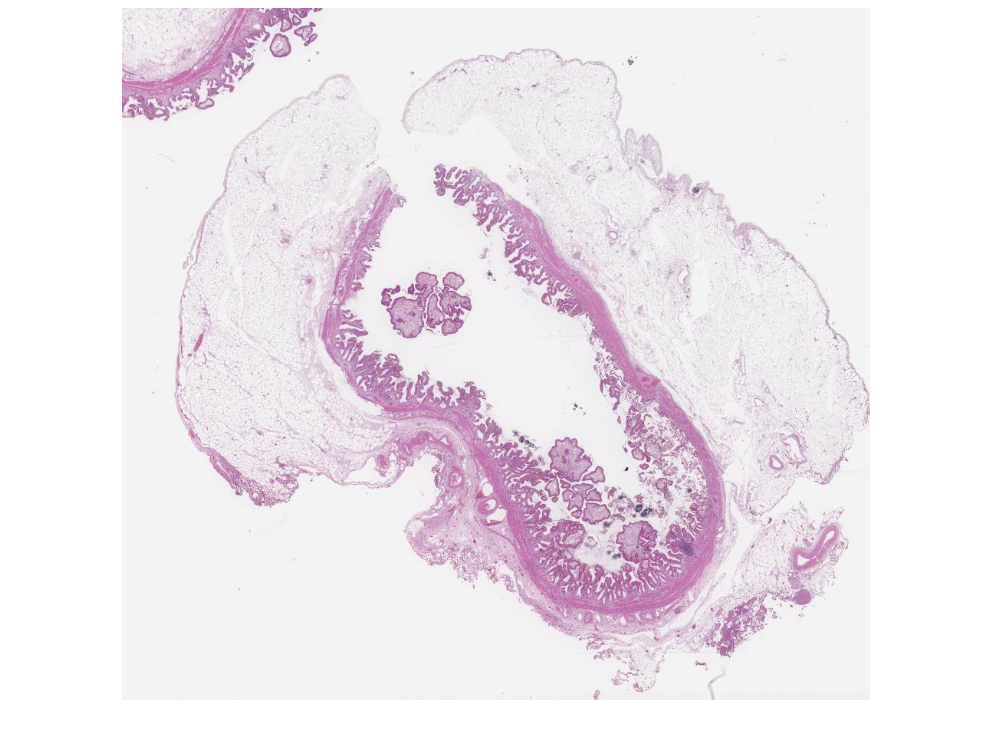
\includegraphics[width=0.25\textwidth,height=\textheight]{./screenshots/thumbnail_cholesterolpolyp.png}}
\href{https://images.patolojiatlasi.com/cholesterolpolyp/HE.html}{Tam
Ekran Görmek İçin Resmi Tıklayın}

\hypertarget{sec-glikojen-depo-hastaligi}{%
\section{Glikojen Depo Hastalığı}\label{sec-glikojen-depo-hastaligi}}

\hypertarget{he}{%
\subsection{HE}\label{he}}

\textbf{Karaciğer İğnde Biyopsisinde glikojen depo hastalığı}

\textbf{Hematoksilen Eozin}

\href{https://images.patolojiatlasi.com/glycogenstorage/HE.html}{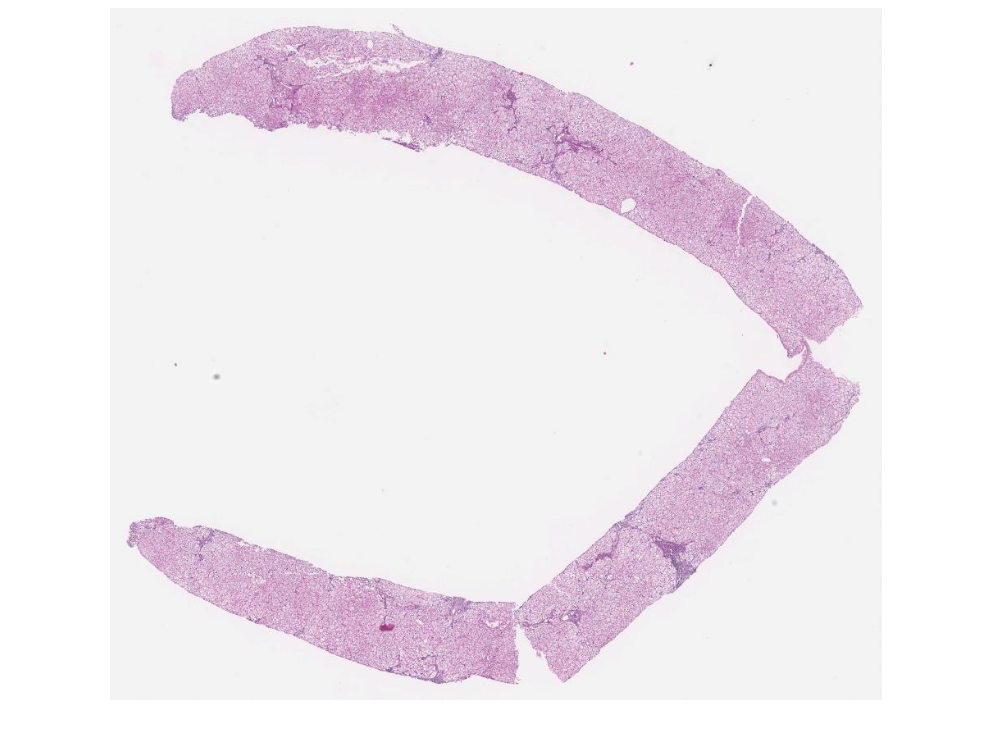
\includegraphics[width=0.25\textwidth,height=\textheight]{./screenshots/thumbnail_glycogenstorage-HE.png}}
\href{https://images.patolojiatlasi.com/glycogenstorage/HE.html}{Tam
Ekran Görmek İçin Resmi Tıklayın}

\hypertarget{pas}{%
\subsection{PAS}\label{pas}}

\textbf{PAS}

\href{https://images.patolojiatlasi.com/glycogenstorage/PAS.html}{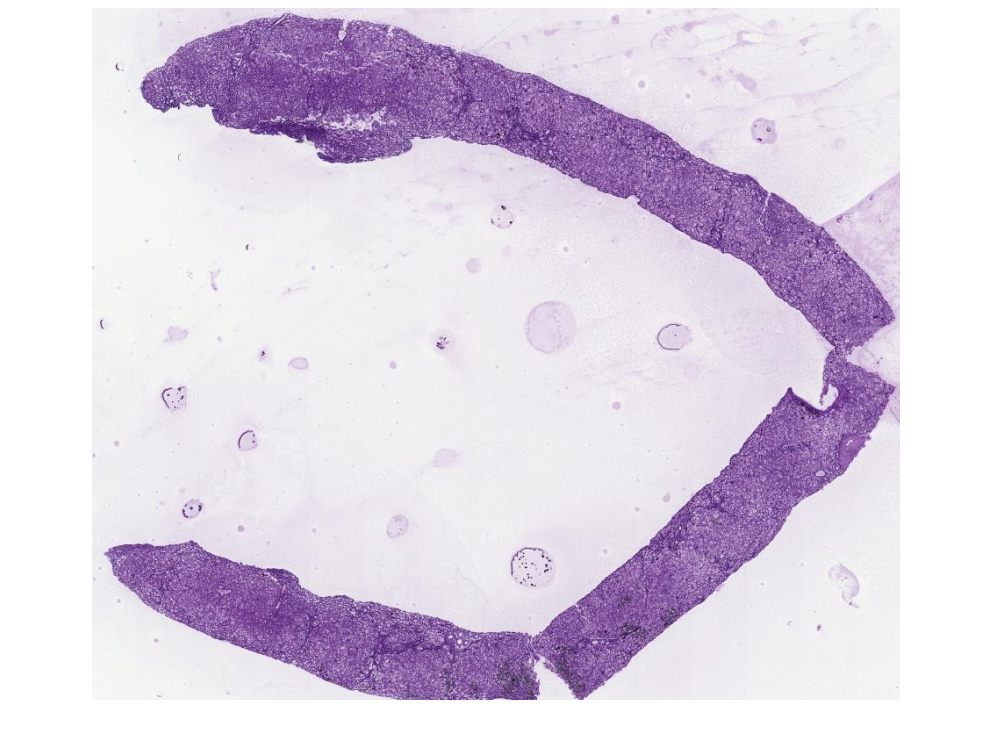
\includegraphics[width=0.25\textwidth,height=\textheight]{./screenshots/thumbnail_glycogenstorage-PAS.png}}
\href{https://images.patolojiatlasi.com/glycogenstorage/PAS.html}{Tam
Ekran Görmek İçin Resmi Tıklayın}

\hypertarget{pasd}{%
\subsection{PASD}\label{pasd}}

\textbf{PASD}

\href{https://images.patolojiatlasi.com/glycogenstorage/PASD.html}{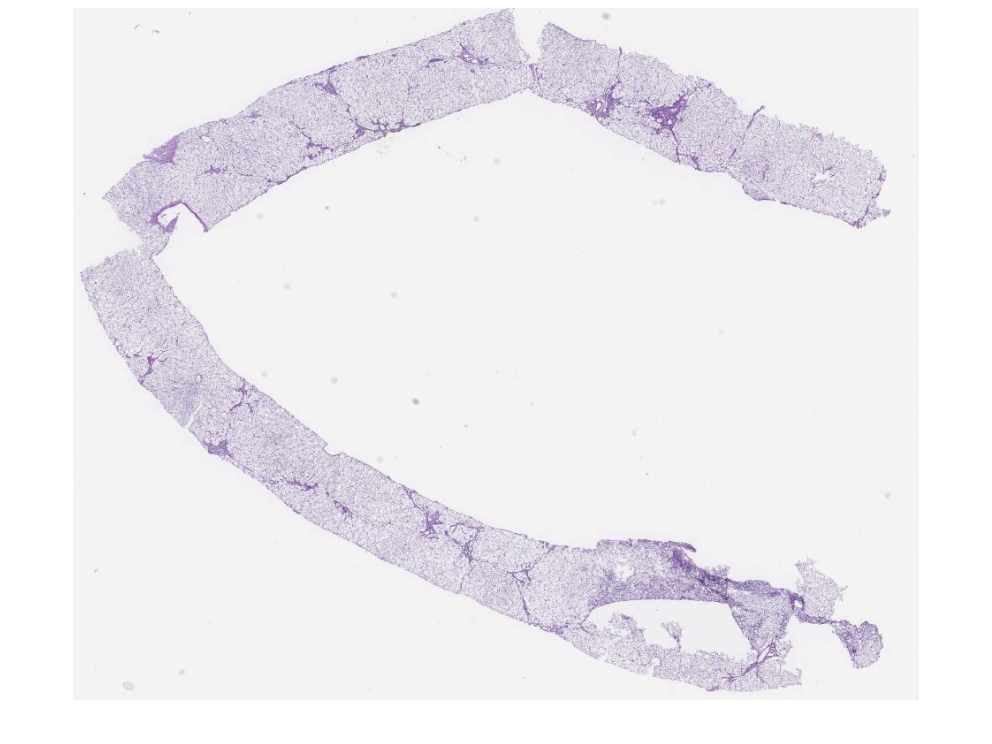
\includegraphics[width=0.25\textwidth,height=\textheight]{./screenshots/thumbnail_glycogenstorage-PASD.png}}
\href{https://images.patolojiatlasi.com/glycogenstorage/PASD.html}{Tam
Ekran Görmek İçin Resmi Tıklayın}

\hypertarget{sec-antrakoz-antrakotik-pigment}{%
\section{Antrakoz, Antrakotik
Pigment}\label{sec-antrakoz-antrakotik-pigment}}

Torakal bölge lenf nodunda antrakotik pigment

\hypertarget{he1}{%
\subsection{HE1}\label{he1}}

\href{https://images.patolojiatlasi.com/anthracosis/HE.html}{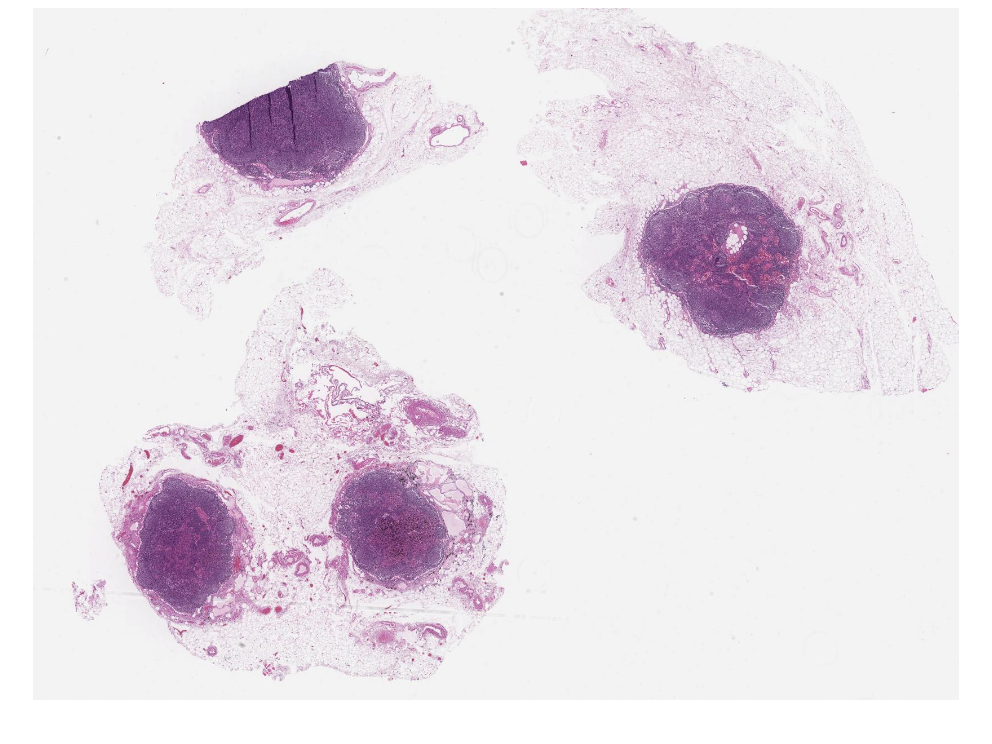
\includegraphics[width=0.25\textwidth,height=\textheight]{./screenshots/thumbnail_anthracosis1.png}}
\href{https://images.patolojiatlasi.com/anthracosis/HE.html}{Click for
Full Screen WSI}

\hypertarget{he2}{%
\subsection{HE2}\label{he2}}

\href{https://images.patolojiatlasi.com/anthracosis/HE2.html}{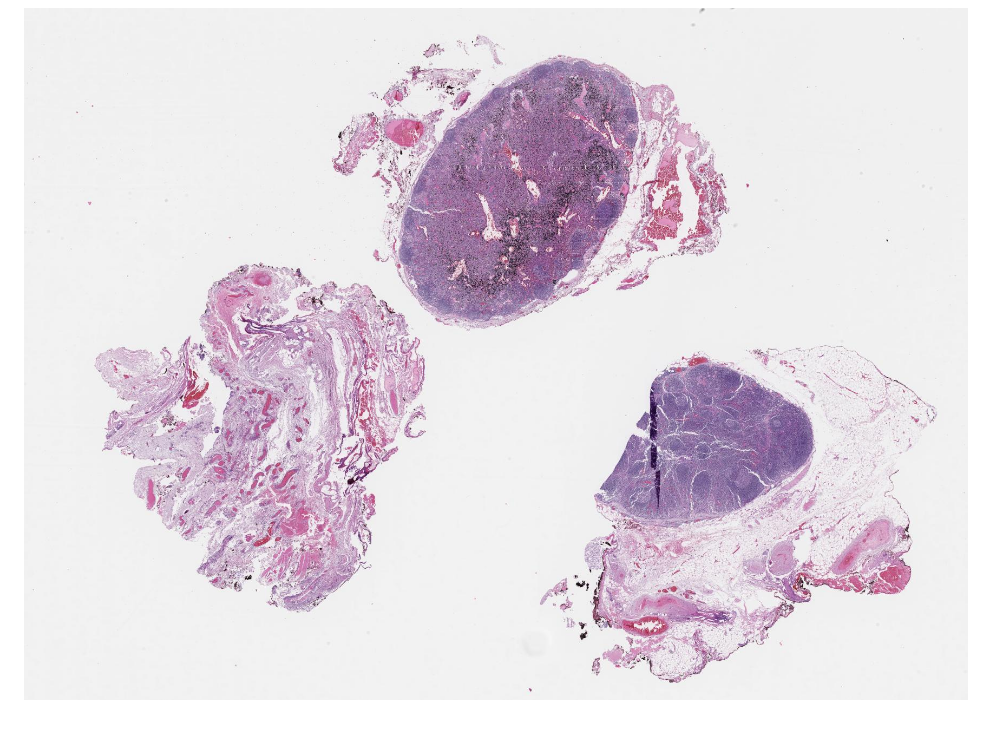
\includegraphics[width=0.25\textwidth,height=\textheight]{./screenshots/thumbnail_anthracosis2.png}}
\href{https://images.patolojiatlasi.com/anthracosis/HE2.html}{Click for
Full Screen WSI}

\hypertarget{sec-melanosis-coli}{%
\section{Melanosis Coli}\label{sec-melanosis-coli}}

\hypertarget{he-1}{%
\subsection{HE}\label{he-1}}

\textbf{Melanozis Koli}

\href{https://images.patolojiatlasi.com/melanosiscoli/HE.html}{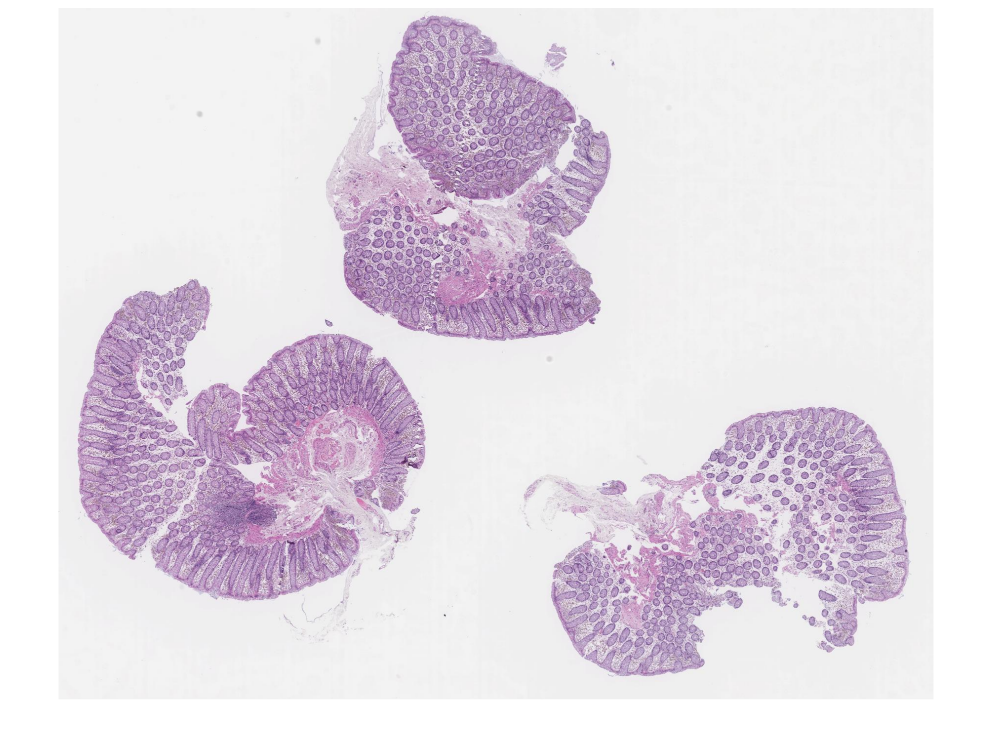
\includegraphics[width=0.25\textwidth,height=\textheight]{./screenshots/thumbnail_melanosiscoli-HE.png}}
\href{https://images.patolojiatlasi.com/melanosiscoli/HE.html}{Tam Ekran
Görmek İçin Resmi Tıklayın}

\hypertarget{pas-1}{%
\subsection{PAS}\label{pas-1}}

\textbf{Melanozis Koli PAS}

\href{https://images.patolojiatlasi.com/melanosiscoli/PAS.html}{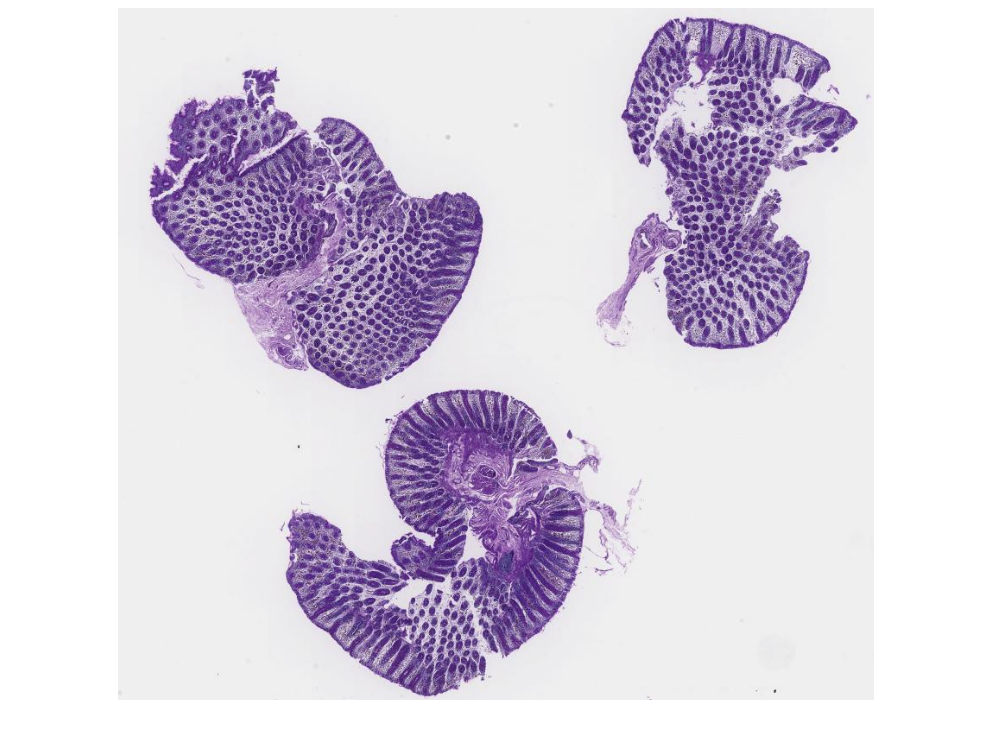
\includegraphics[width=0.25\textwidth,height=\textheight]{./screenshots/thumbnail_melanosiscoli-PAS.png}}
\href{https://images.patolojiatlasi.com/melanosiscoli/PAS.html}{Tam
Ekran Görmek İçin Resmi Tıklayın}

\{.content-hidden unless-format=``epub''\}

\hypertarget{he-2}{%
\subsection{HE}\label{he-2}}

\textbf{Melanozis Koli}

\href{https://images.patolojiatlasi.com/melanosiscoli/HE.html}{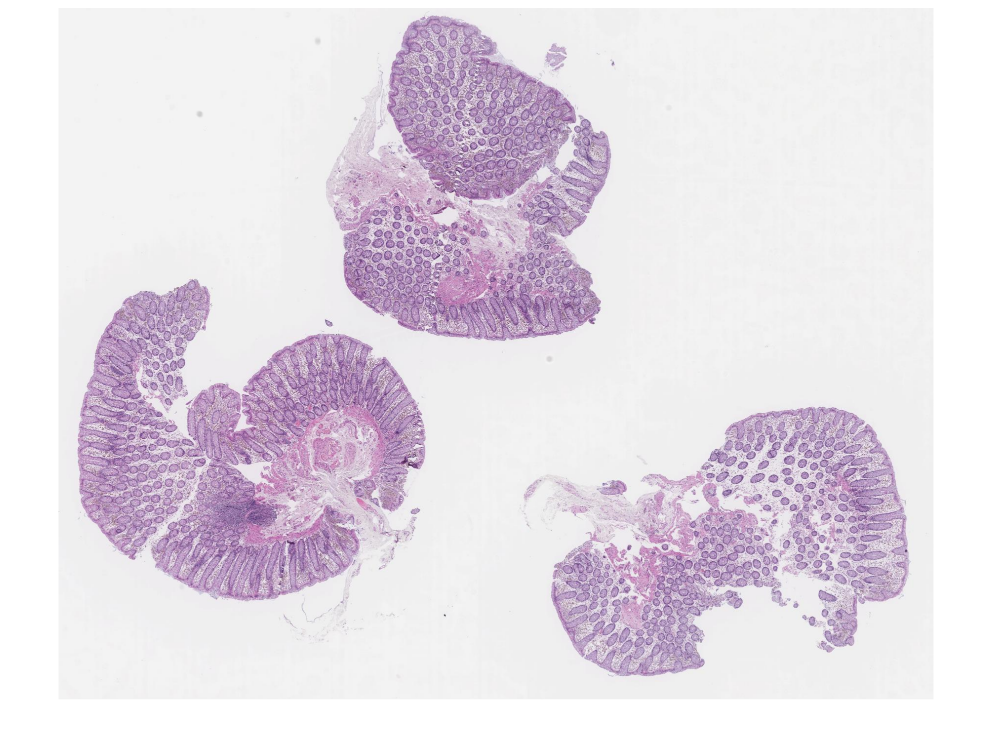
\includegraphics[width=0.25\textwidth,height=\textheight]{./screenshots/thumbnail_melanosiscoli-HE.png}}
\href{https://images.patolojiatlasi.com/melanosiscoli/HE.html}{Tam Ekran
Görmek İçin Resmi Tıklayın}

\hypertarget{pas-2}{%
\subsection{PAS}\label{pas-2}}

\textbf{Melanozis Koli PAS}

\href{https://images.patolojiatlasi.com/melanosiscoli/PAS.html}{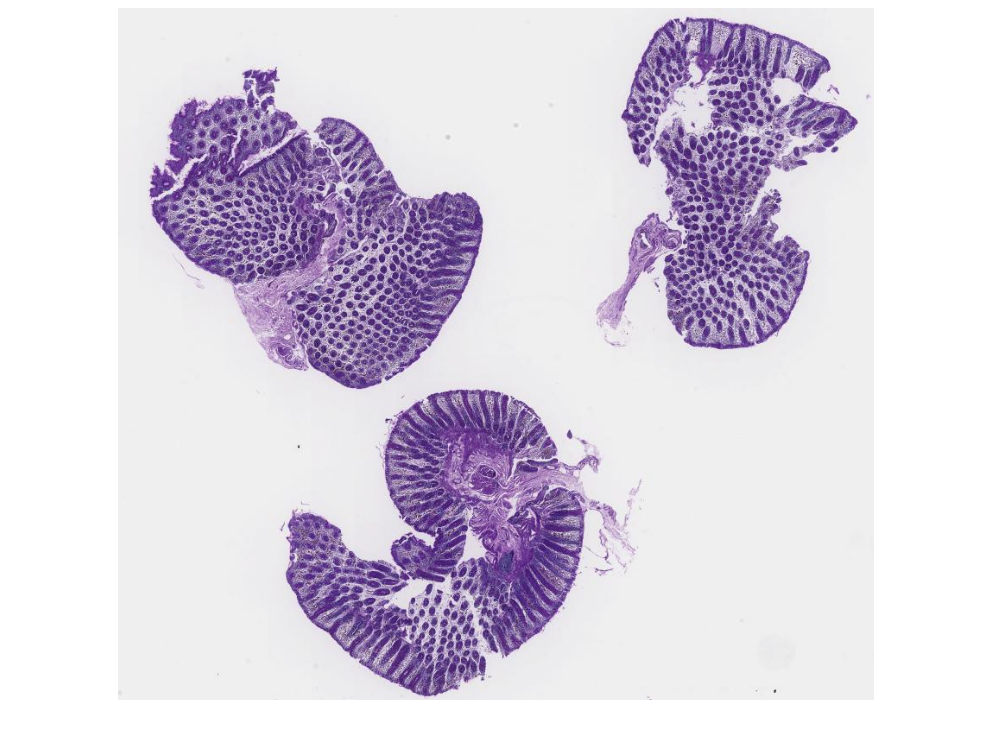
\includegraphics[width=0.25\textwidth,height=\textheight]{./screenshots/thumbnail_melanosiscoli-PAS.png}}
\href{https://images.patolojiatlasi.com/melanosiscoli/PAS.html}{Tam
Ekran Görmek İçin Resmi Tıklayın}

\hypertarget{sec-hucre-disi-birikimler}{%
\chapter{Hücre Dışı Birikimler}\label{sec-hucre-disi-birikimler}}

\hypertarget{sec-okronozis}{%
\section{Okronozis}\label{sec-okronozis}}

\textbf{Okronozis}

\href{https://images.patolojiatlasi.com/ochronosis/HE.html}{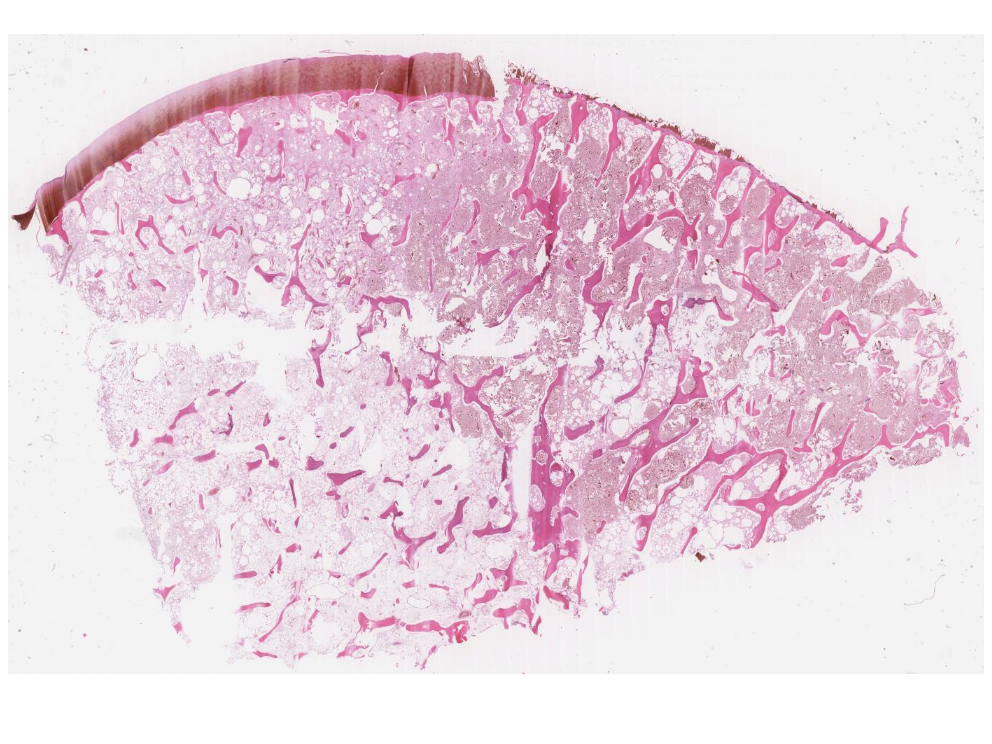
\includegraphics[width=0.25\textwidth,height=\textheight]{./screenshots/thumbnail_ochronosis.png}}
\href{https://images.patolojiatlasi.com/ochronosis/HE.html}{Tam Ekran
Görmek İçin Resmi Tıklayın}

\hypertarget{sec-hucre-hasari}{%
\chapter{Hücre Hasarı}\label{sec-hucre-hasari}}

\hypertarget{sec-reaktif-atipi}{%
\section{Reaktif Atipi, ülsere kolon polibi}\label{sec-reaktif-atipi}}

\textbf{Reaktif Atipi, ülsere kolon polibi}

\href{https://images.patolojiatlasi.com/reactive-atypia/HE.html}{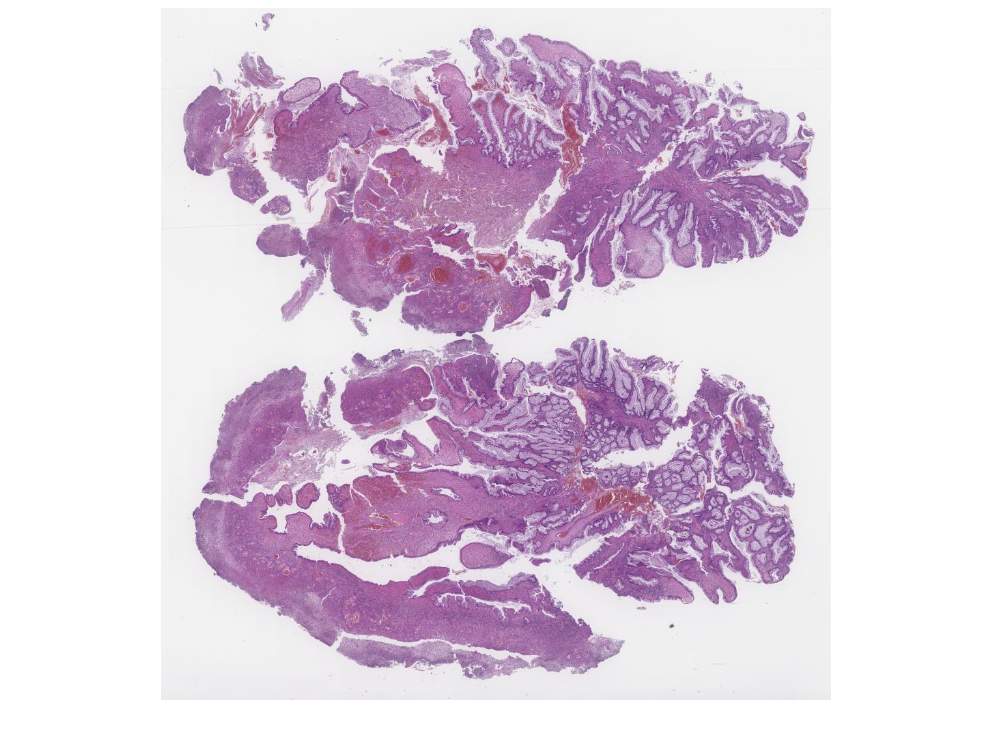
\includegraphics[width=0.25\textwidth,height=\textheight]{./screenshots/thumbnail_reactive-atypia.png}}
\href{https://images.patolojiatlasi.com/reactive-atypia/HE.html}{Tam
Ekran Görmek İçin Resmi Tıklayın}

\hypertarget{sec-iskemi-ve-nekroz}{%
\chapter{İskemi ve Nekroz}\label{sec-iskemi-ve-nekroz}}

\hypertarget{sec-yag-nekrozu-sabunlasma}{%
\subsection{Yağ nekrozu ve
Sabunlaşma}\label{sec-yag-nekrozu-sabunlasma}}

\textbf{Yağ dokuda yağ nekrozu ve sabunlaşma}

\href{https://images.patolojiatlasi.com/fat-necrosis/HE.html}{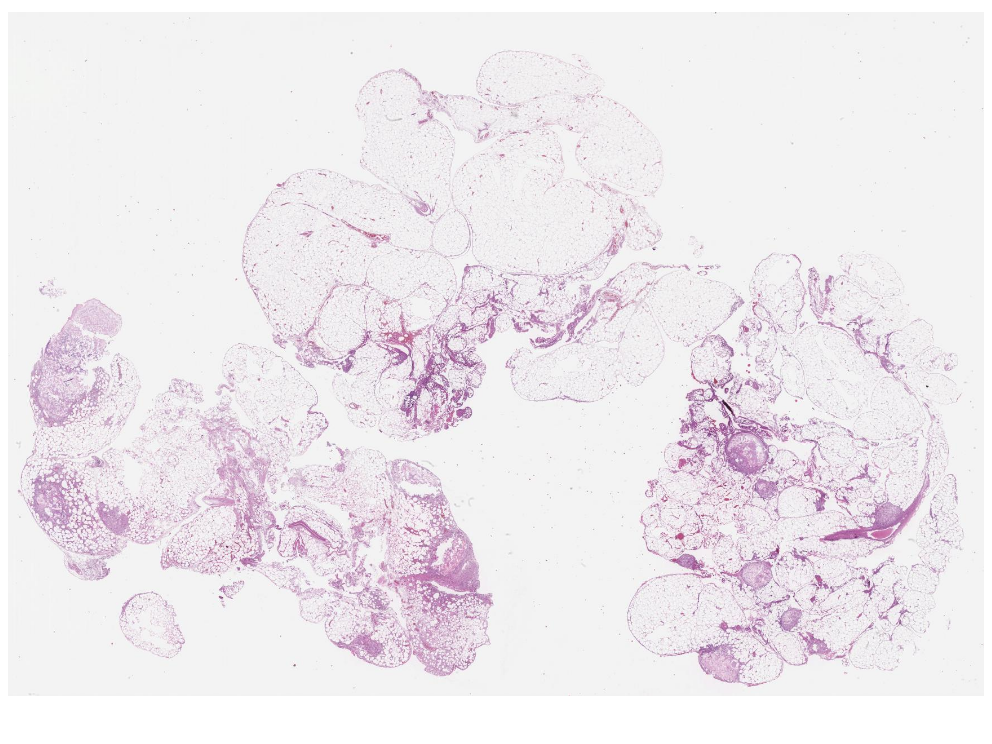
\includegraphics[width=0.25\textwidth,height=\textheight]{./screenshots/thumbnail_fat-necrosis.png}}
\href{https://images.patolojiatlasi.com/fat-necrosis/HE.html}{Tam Ekran
Görmek İçin Resmi Tıklayın}

\hypertarget{sec-congestion-spleen}{%
\chapter{Dalak konjesyon}\label{sec-congestion-spleen}}

\textbf{Dalak konjesyon}

\href{https://images.patolojiatlasi.com/congestion-spleen/HE.html}{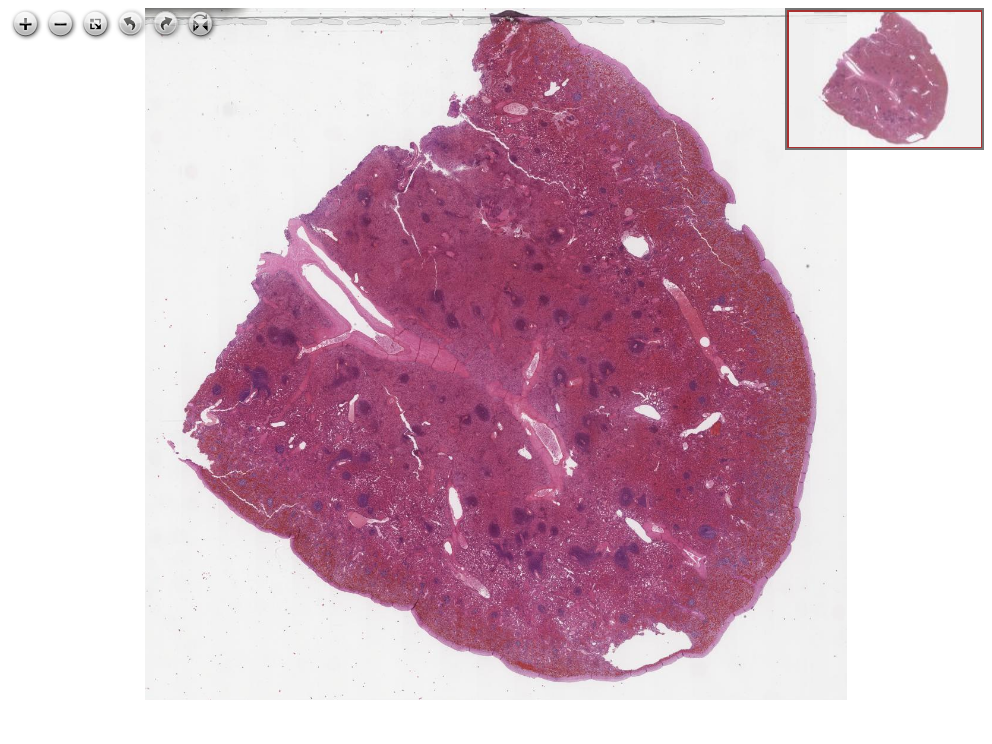
\includegraphics[width=0.25\textwidth,height=\textheight]{./screenshots/thumbnail_congestion-spleen.png}}
\href{https://images.patolojiatlasi.com/congestion-spleen/HE.html}{Tam
Ekran Görmek İçin Resmi Tıklayın}

\hypertarget{sec-amiloidoz}{%
\chapter{Amiloidoz (Amiloid Birikimi)}\label{sec-amiloidoz}}

\hypertarget{sec-amiloidoz-kristal-viyole}{%
\section{Kristal Viyole}\label{sec-amiloidoz-kristal-viyole}}

\textbf{Damar duvarlarında amiloid birikimi}

\href{https://images.patolojiatlasi.com/amyloid/crystalviolet.html}{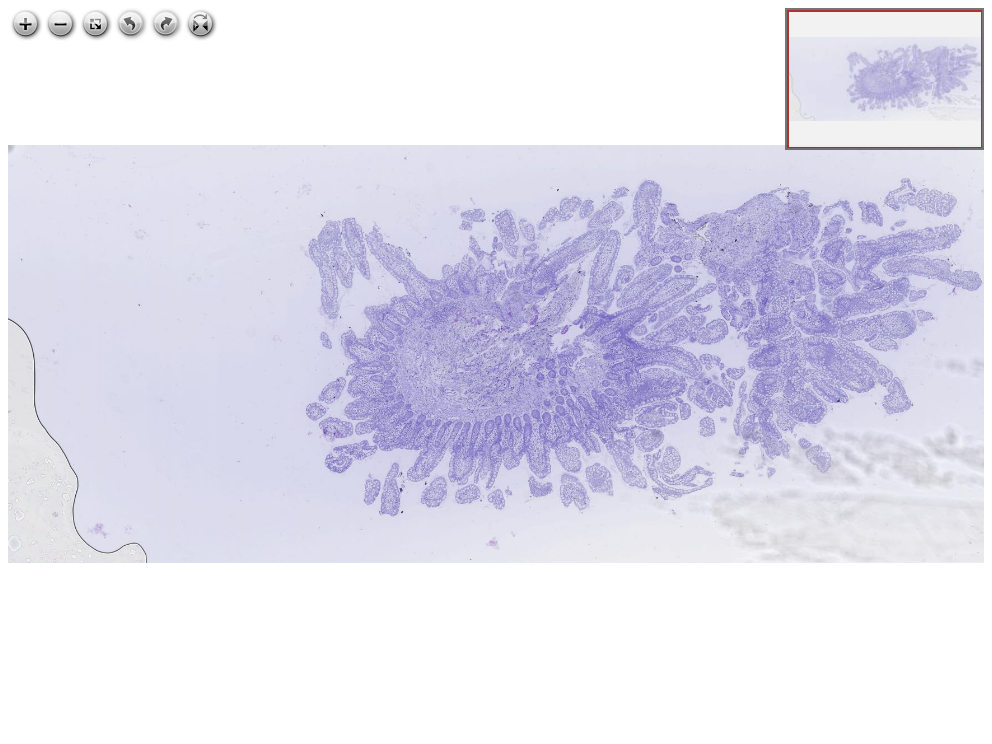
\includegraphics[width=0.25\textwidth,height=\textheight]{./screenshots/thumbnail_crystalviolet.png}}
\href{https://images.patolojiatlasi.com/amyloid/crystalviolet.html}{Tam
Ekran Görmek İçin Resmi Tıklayın}

\hypertarget{sec-amiloidoz-kongo-kirmizisi}{%
\section{Kongo Kırmızısı}\label{sec-amiloidoz-kongo-kirmizisi}}

\textbf{Congo Red stain for amyloidosis}

\href{https://images.patolojiatlasi.com/congored/congored.html}{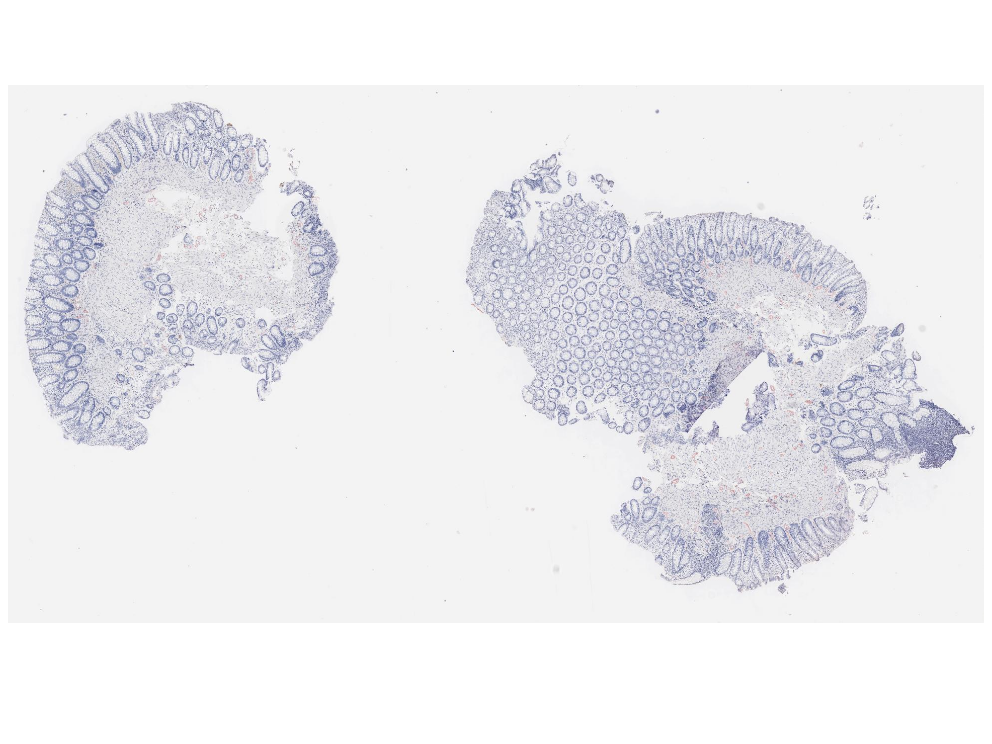
\includegraphics[width=0.25\textwidth,height=\textheight]{./screenshots/thumbnail_congored.png}}
\href{https://images.patolojiatlasi.com/congored/congored.html}{Tam
Ekran Görmek İçin Resmi Tıklayın}

\hypertarget{sec-amiloidoz-kongo-kirmizisi-cift-kiricilik}{%
\section{Kongo Kırmızısı Çift
Kırıcılık}\label{sec-amiloidoz-kongo-kirmizisi-cift-kiricilik}}

\url{https://www.youtube.com/watch?v=U9glkfQLTm4}

\textbf{Congo Red Birefringence}

\href{https://www.youtube.com/watch?v=U9glkfQLTm4}{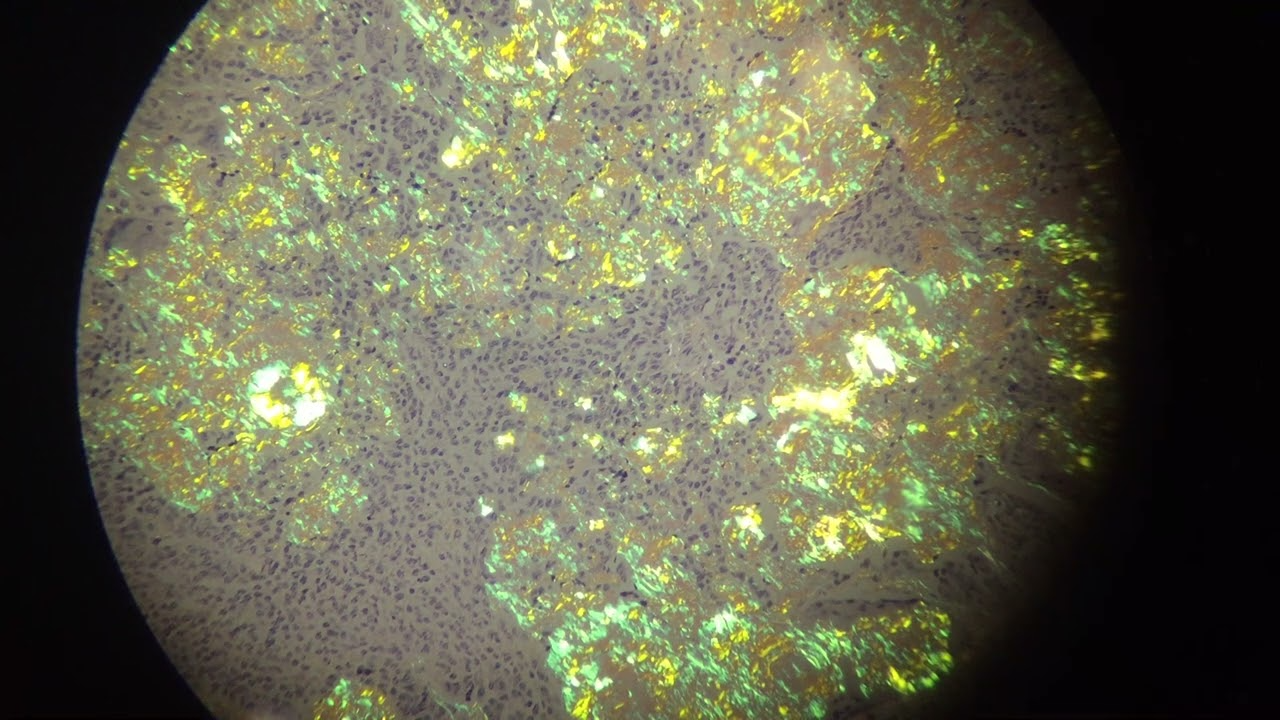
\includegraphics[width=0.25\textwidth,height=\textheight]{./screenshots/thumbnail_congored_video.png}}
\href{https://www.youtube.com/watch?v=U9glkfQLTm4}{Video İçin Tıklayın}

\hypertarget{sec-tamir-mekanizmalari}{%
\chapter{Tamir Mekanizmaları}\label{sec-tamir-mekanizmalari}}

Bu sayfadaki görüntülere artırılmış gerçeklik (augmented reality) ile de
ulaşabilirsiniz\footnote{\href{https://github.com/veterinarypathology3d}{Tarık
  Atmaca} tarafından \url{https://veterinarypathology3d.com/}
  geliştirilmiştir.}.

Karekodu cep telefonunuza okutun:

\begin{figure}


\includegraphics[width=1.04167in,height=\textheight]{images/AR-tamir.jpeg} \hfill{}

\end{figure}

Link ile açılan sayfaya ve kamera erişimine izin verin. Sonra kamerayı
bu sayfadaki patoloji resimlerine tutun. Tanılar cep telefonunuzda
görünecektir.

\url{https://www.youtube.com/watch?v=76bOJIiT29Y}

\hypertarget{sec-fibrozis}{%
\section{Fibrozis}\label{sec-fibrozis}}

Kolesistit spesmeninde gelişmekte olan genç fibrozis

\href{https://images.patolojiatlasi.com/fibrosis/HE.html}{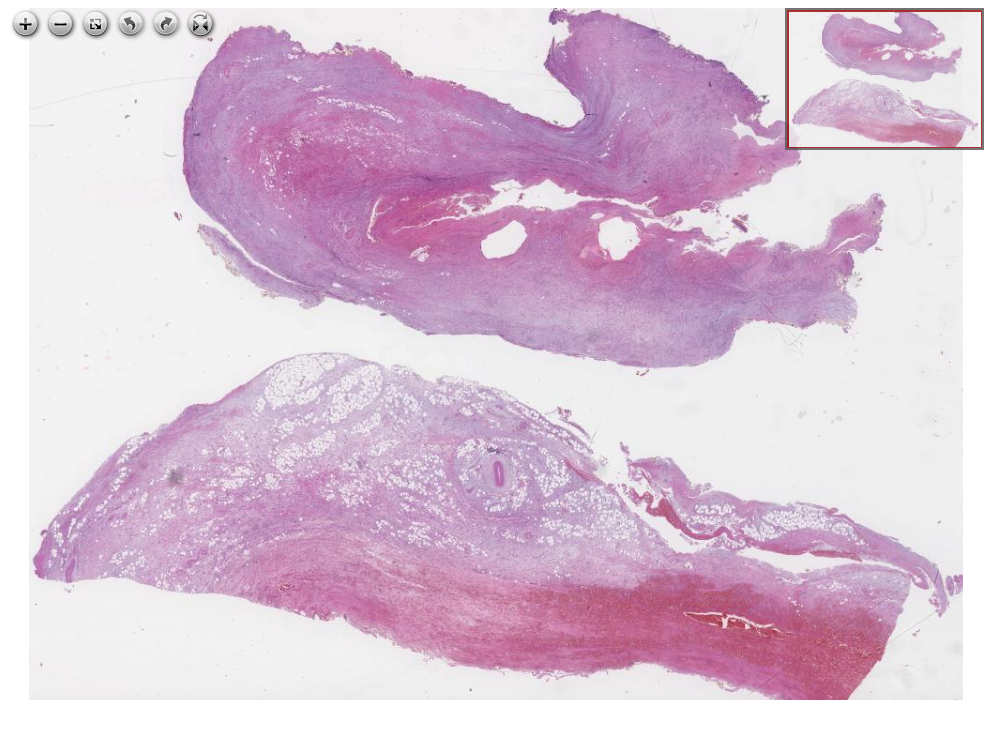
\includegraphics[width=0.25\textwidth,height=\textheight]{./screenshots/thumbnail_fibrosis.png}}
\href{https://images.patolojiatlasi.com/fibrosis/HE.html}{Tam Ekran
Görmek İçin Resmi Tıklayın}

\hypertarget{sec-keloid-skar}{%
\section{Keloid - Skar}\label{sec-keloid-skar}}

Keloid Skar oluşumu

\href{https://images.patolojiatlasi.com/keloid-scar/HE.html}{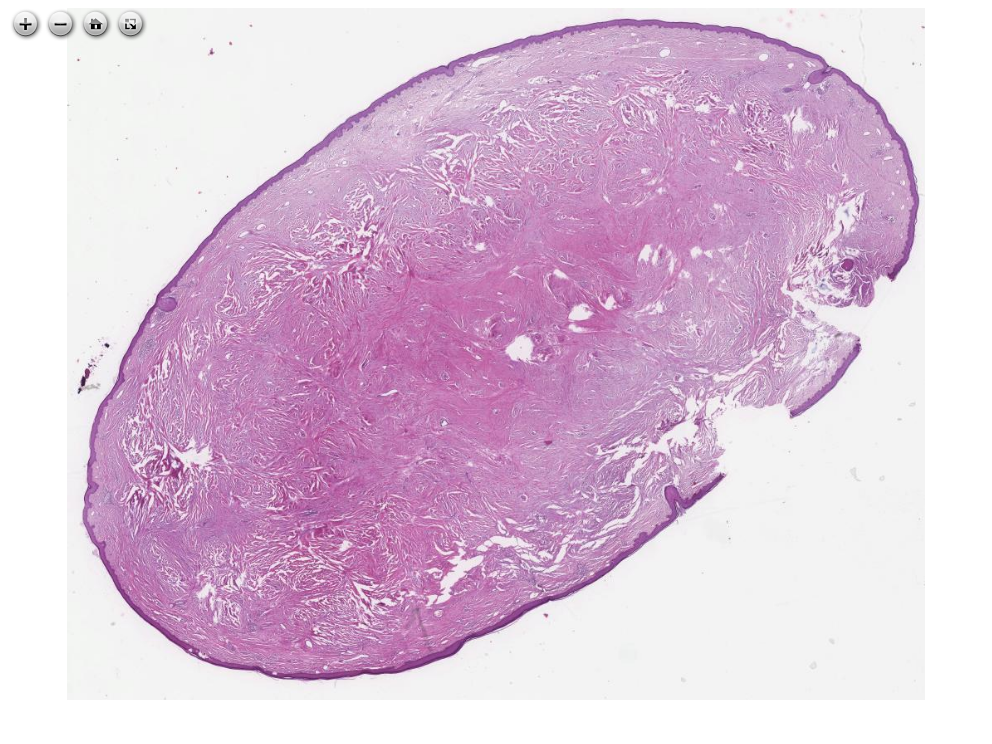
\includegraphics[width=0.25\textwidth,height=\textheight]{./screenshots/thumbnail_keloid-scar.png}}
\href{https://images.patolojiatlasi.com/keloid-scar/HE.html}{Tam Ekran
Görmek İçin Resmi Tıklayın}

\hypertarget{sec-erozyon}{%
\chapter{Erozyon}\label{sec-erozyon}}

\hypertarget{sec-mide-mukozasinda-erozyon}{%
\section{Mide mukozasında erozyon}\label{sec-mide-mukozasinda-erozyon}}

\textbf{Mide mukozasında erozyon}

\href{https://images.patolojiatlasi.com/erosion/HE.html}{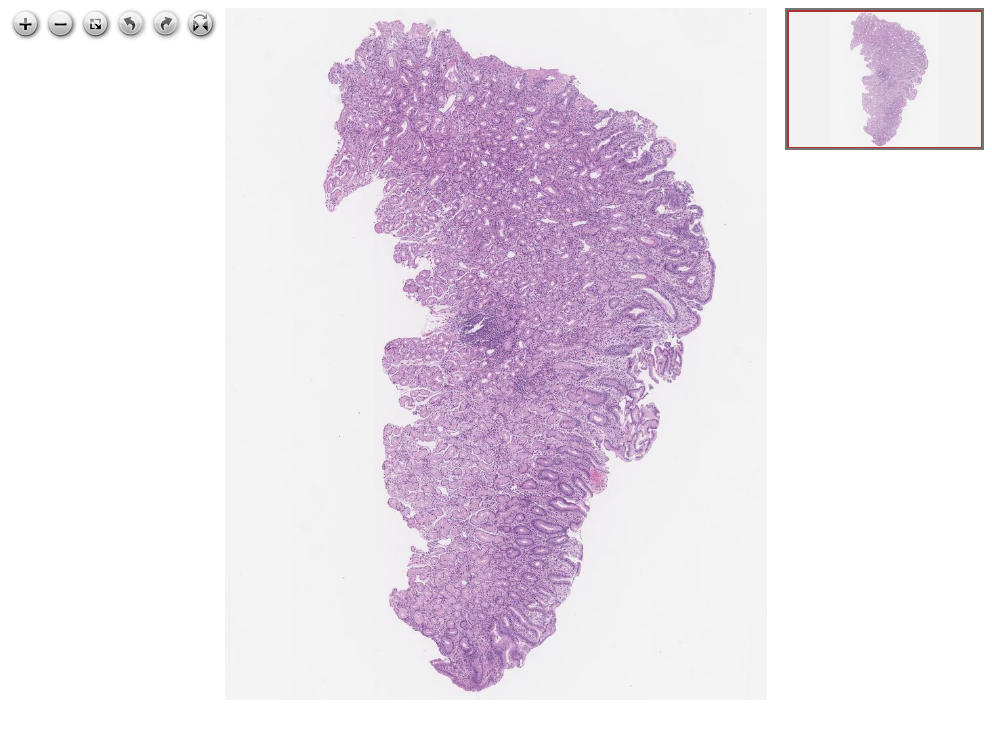
\includegraphics[width=0.25\textwidth,height=\textheight]{./screenshots/thumbnail_erosion.png}}
\href{https://images.patolojiatlasi.com/erosion/HE.html}{Tam Ekran
Görmek İçin Resmi Tıklayın}

\part{İnflamasyon}

\hypertarget{sec-akut-inflamasyon}{%
\chapter{Akut İnflamasyon}\label{sec-akut-inflamasyon}}

\hypertarget{sec-akut-appendisit}{%
\section{Akut Appendisit}\label{sec-akut-appendisit}}

\hypertarget{he-3}{%
\subsection{HE}\label{he-3}}

\textbf{Akut appendisit}


\includegraphics[width=0.15\textwidth,height=\textheight]{index_files/mediabag/qrcodes/acute-appendicitis-HE_qrcode.pdf}
\href{https://images.patolojiatlasi.com/acute-appendicitis/HE.html}{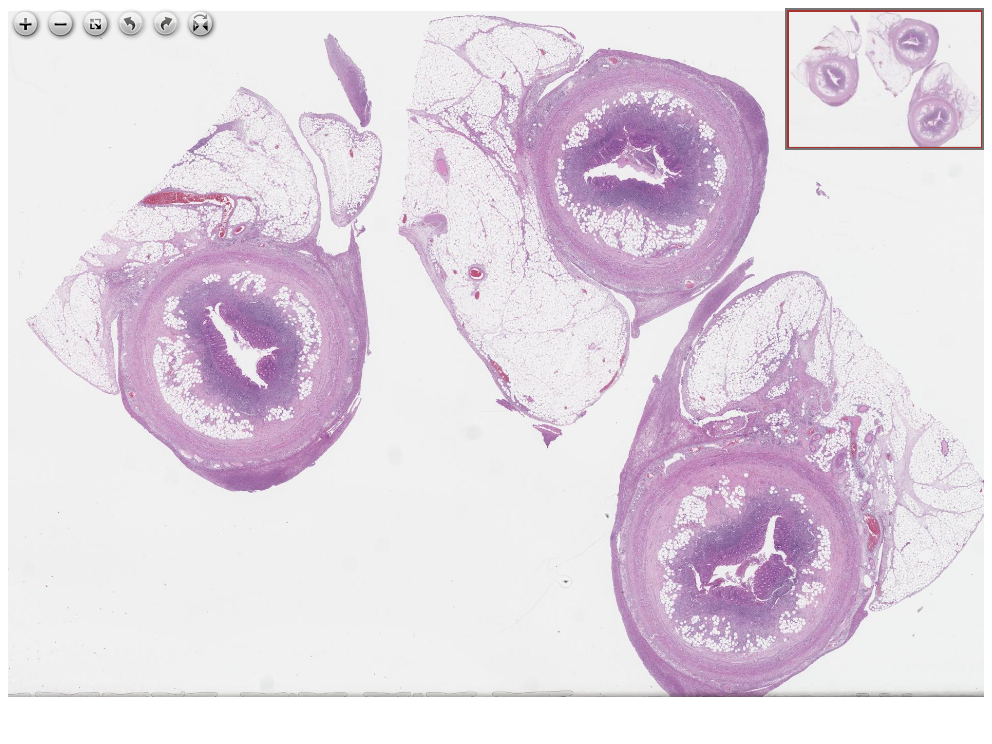
\includegraphics[width=0.25\textwidth,height=\textheight]{./screenshots/thumbnail_acute-appendicitis.png}}
\href{https://images.patolojiatlasi.com/acute-appendicitis/HE.html}{Tam
Ekran Görmek İçin Resmi Tıklayın}

\hypertarget{sec-kronik-inflamasyon}{%
\chapter{Kronik İnflamasyon}\label{sec-kronik-inflamasyon}}

\hypertarget{sec-hidronefroz-kronik-pyelonefrit}{%
\section{Hidronefroz ve Kronik
Pyelonefrit}\label{sec-hidronefroz-kronik-pyelonefrit}}

\textbf{Hidronefroz ve Kronik Pyelonefrit}

\href{https://images.patolojiatlasi.com/chronicpyelonephritis/HE1.html}{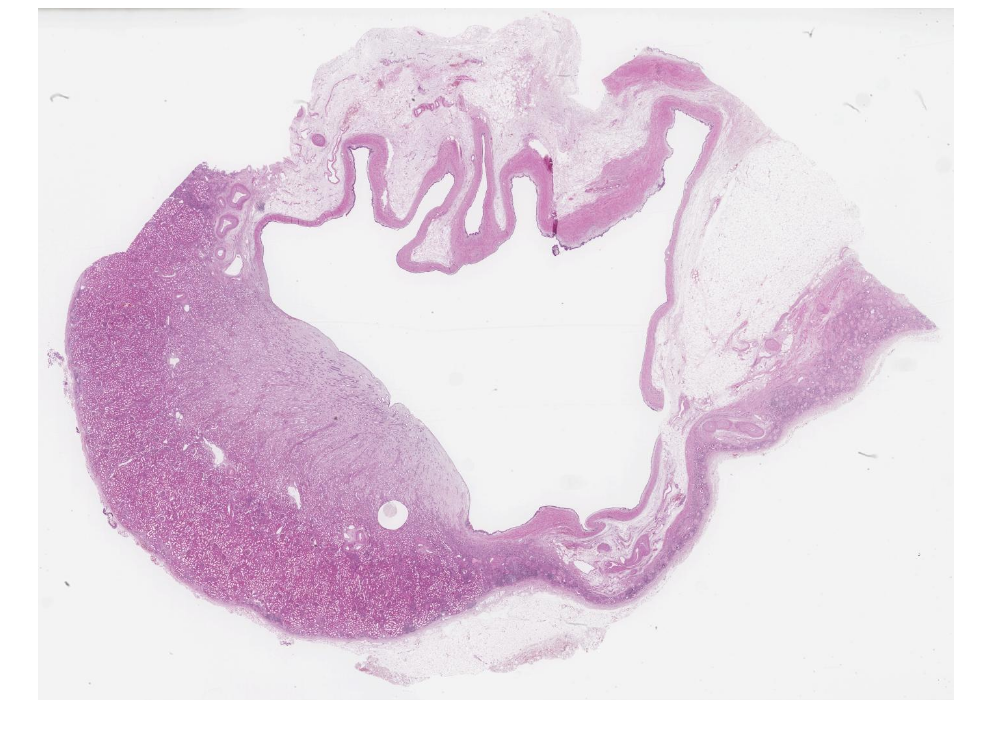
\includegraphics[width=0.25\textwidth,height=\textheight]{./screenshots/thumbnail_chronicpyelonephritis-1.png}}
\href{https://images.patolojiatlasi.com/chronicpyelonephritis/HE1.html}{Tam
Ekran Görmek İçin Resmi Tıklayın}

\textbf{Hidronefroz ve Kronik Pyelonefrit}

\href{https://images.patolojiatlasi.com/chronicpyelonephritis/HE2.html}{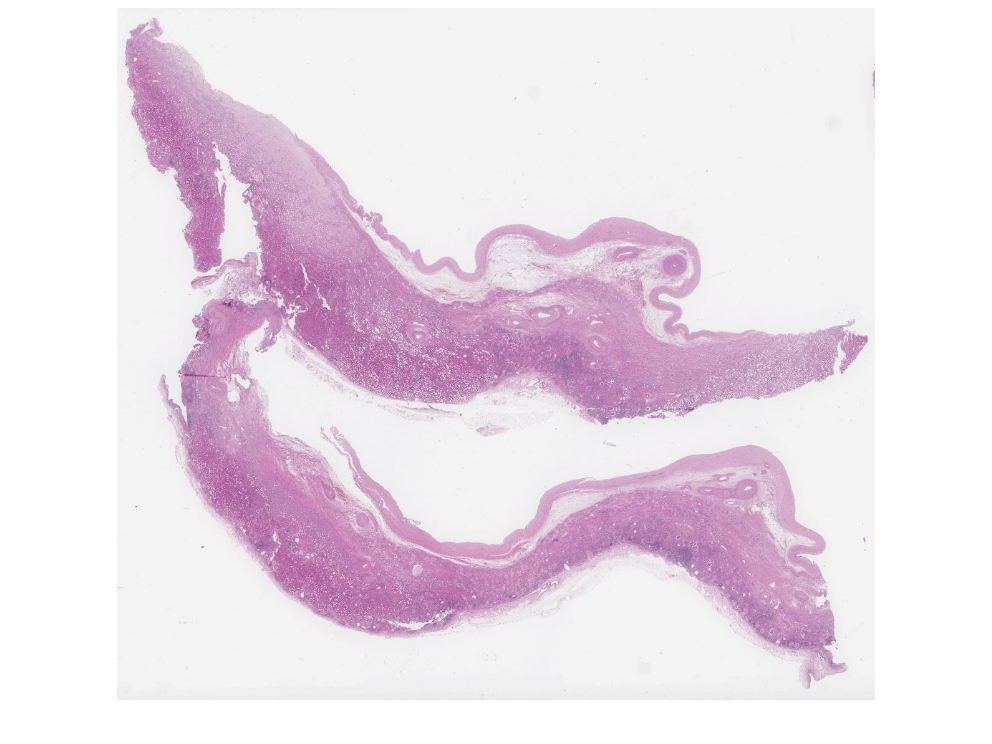
\includegraphics[width=0.25\textwidth,height=\textheight]{./screenshots/thumbnail_chronicpyelonephritis-2.png}}
\href{https://images.patolojiatlasi.com/chronicpyelonephritis/HE2.html}{Tam
Ekran Görmek İçin Resmi Tıklayın}

\hypertarget{sec-kronik-pyelonefrit}{%
\section{Kronik Pyelonefrit}\label{sec-kronik-pyelonefrit}}

\textbf{Kronik Pyelonefrit}

\href{https://images.patolojiatlasi.com/chronic-pyelonephritis/HE.html}{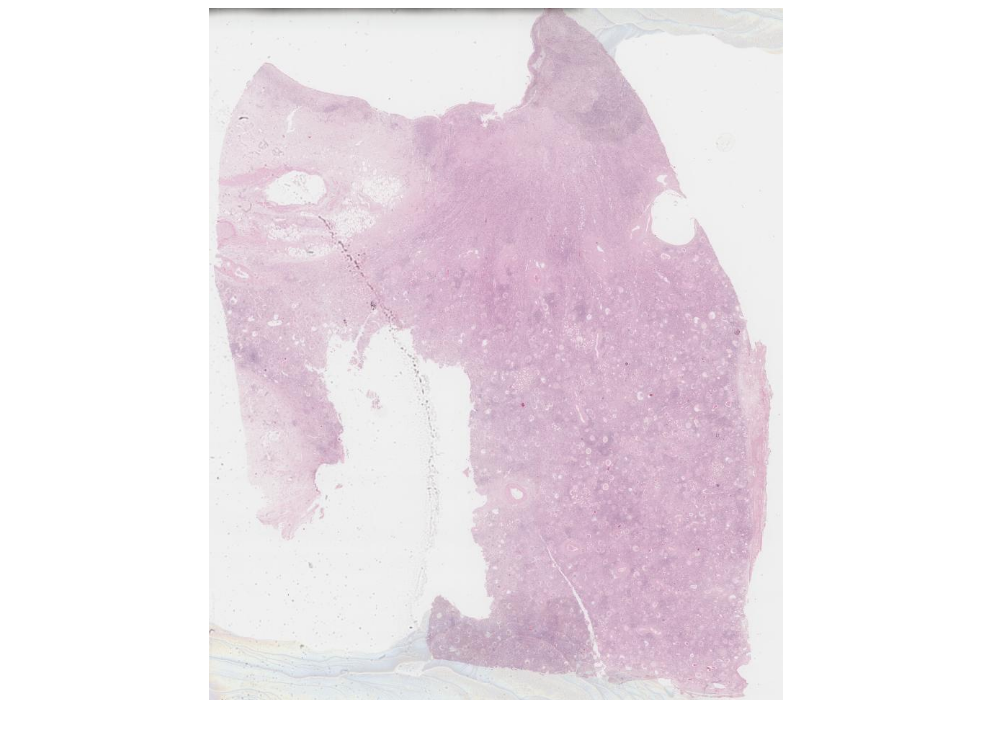
\includegraphics[width=0.25\textwidth,height=\textheight]{./screenshots/thumbnail_chronic-pyelonephritis.png}}
\href{https://images.patolojiatlasi.com/chronic-pyelonephritis/HE.html}{Tam
Ekran Görmek İçin Resmi Tıklayın}

\hypertarget{sec-granulamatoz-inflamasyon}{%
\chapter{Granülamatöz İnflamasyon}\label{sec-granulamatoz-inflamasyon}}

\hypertarget{sec-nekrotizan-granulamatoz-inflamasyon}{%
\section{Nekrotizan Granülamatöz
İnflamasyon}\label{sec-nekrotizan-granulamatoz-inflamasyon}}

\textbf{Karaciğer dokusunda nekrotizan granülamatöz inflamasyon}

\href{https://images.patolojiatlasi.com/necrotisinggranuloma/HE.html}{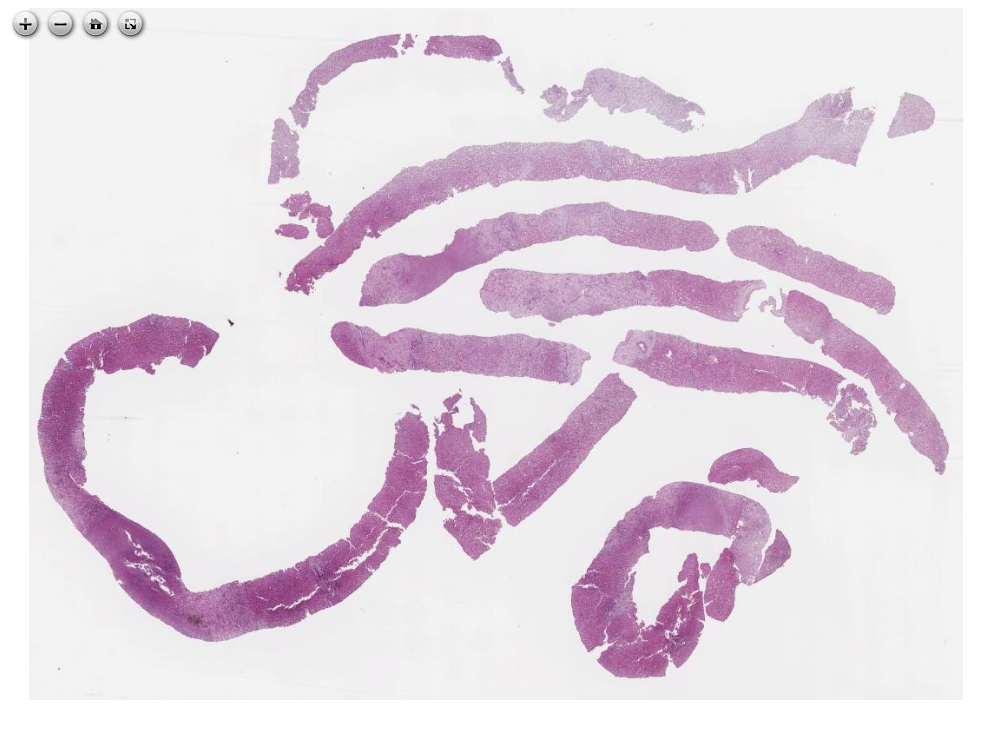
\includegraphics[width=0.25\textwidth,height=\textheight]{./screenshots/thumbnail_necrotisinggranuloma.png}}
\href{https://images.patolojiatlasi.com/necrotisinggranuloma/HE.html}{Tam
Ekran Görmek İçin Resmi Tıklayın}

\part{İnfeksiyöz Hastalıkların Patolojisi}

\hypertarget{sec-viruslar}{%
\chapter{Viruslar}\label{sec-viruslar}}

\hypertarget{sec-herpes-simplex-virus}{%
\section{Herpes Simplex Virus (HSV)}\label{sec-herpes-simplex-virus}}

\href{https://images.patolojiatlasi.com/HSV/herpesesophagitis/viewer_z0.html}{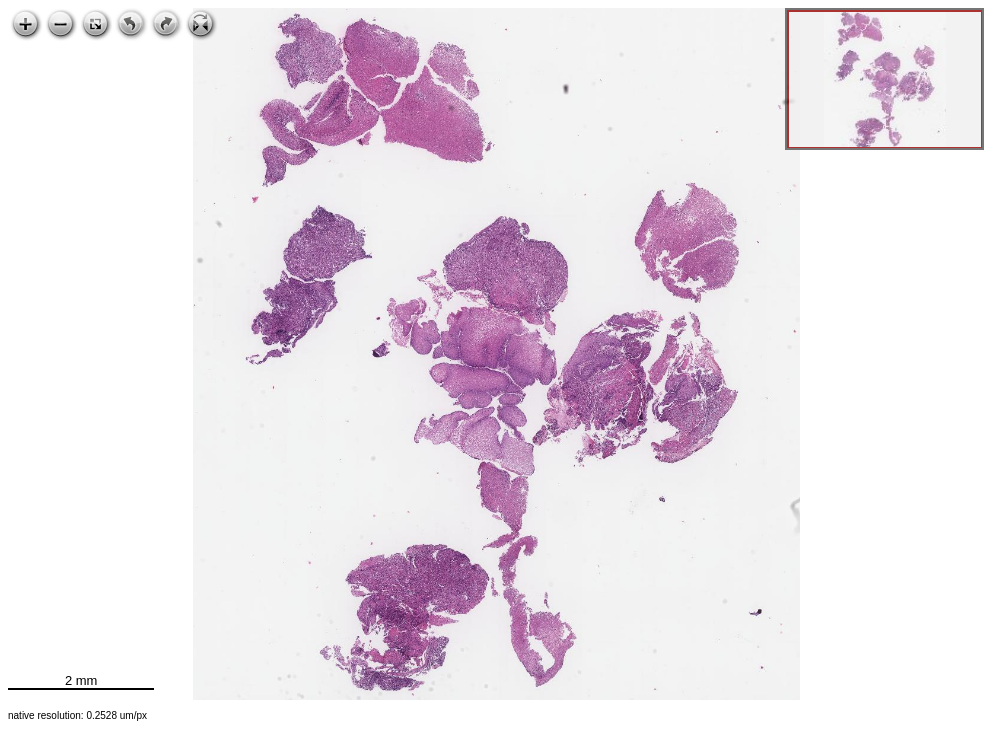
\includegraphics[width=0.25\textwidth,height=\textheight]{./screenshots/thumbnail_herpesesophagitis.png}}
\href{https://images.patolojiatlasi.com/HSV/herpesesophagitis/viewer_z0.html}{Tam
Ekran Görmek İçin Resmi Tıklayın}

\hypertarget{sec-molluscum-contagiosum}{%
\section{Molluscum contagiosum}\label{sec-molluscum-contagiosum}}

\textbf{Molluscum contagiosum}

\href{https://images.patolojiatlasi.com/molluscum-contagiosum/HE.html}{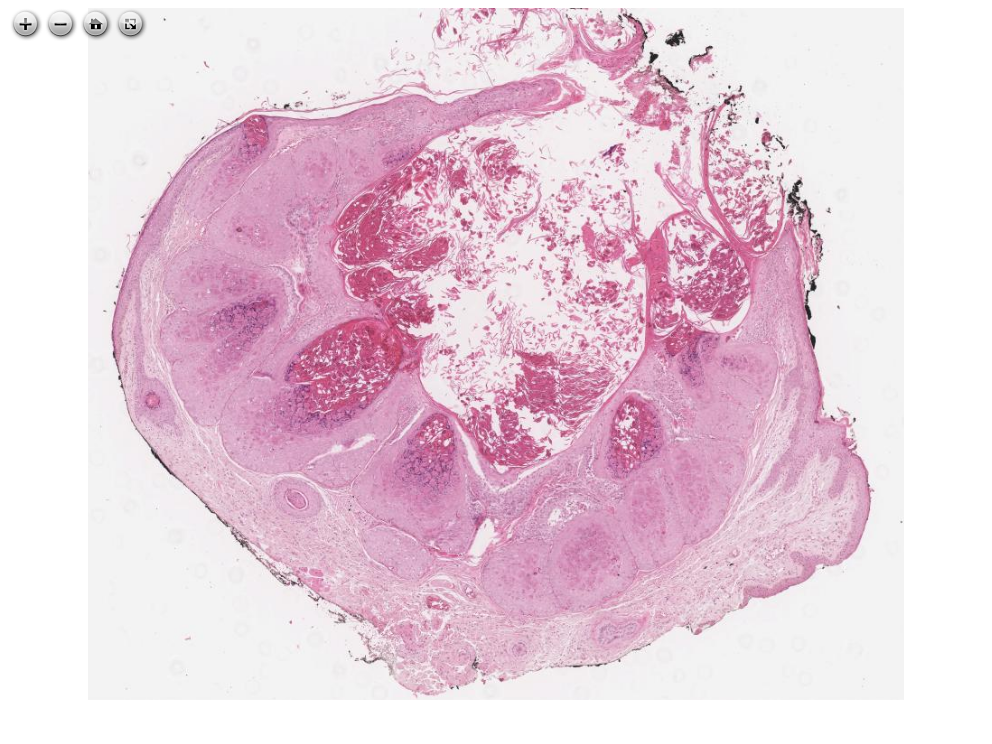
\includegraphics[width=0.25\textwidth,height=\textheight]{./screenshots/thumbnail_molluscum-contagiosum.png}}
\href{https://images.patolojiatlasi.com/molluscum-contagiosum/HE.html}{Tam
Ekran Görmek İçin Resmi Tıklayın}

\hypertarget{sec-bakteriler}{%
\chapter{Bakteriler}\label{sec-bakteriler}}

\hypertarget{sec-helicobacter-pylori}{%
\section{Helicobacter pylori}\label{sec-helicobacter-pylori}}

\hypertarget{he-4}{%
\subsection{HE}\label{he-4}}

\textbf{Mide'de Helicobacter pylori (H. pylori) HE}

\href{https://images.patolojiatlasi.com/helicobacterpylori/HE.html}{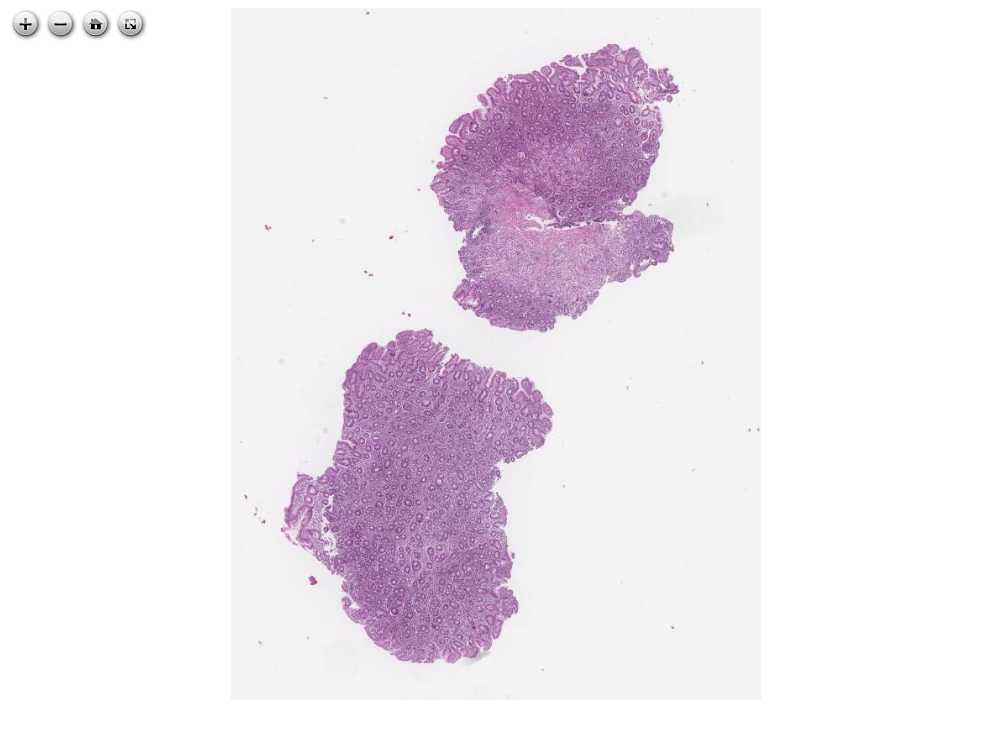
\includegraphics[width=0.25\textwidth,height=\textheight]{./screenshots/thumbnail_helicobacterpylori.png}}
\href{https://images.patolojiatlasi.com/helicobacterpylori/HE.html}{Tam
Ekran Görmek İçin Resmi Tıklayın}

\hypertarget{warthin-starry}{%
\subsection{Warthin-Starry}\label{warthin-starry}}

\textbf{Mide'de Helicobacter pylori (H. pylori) Warthin Starry
Histokimyası}

\href{https://images.patolojiatlasi.com/helicobacterpylori/warthinstarry.html}{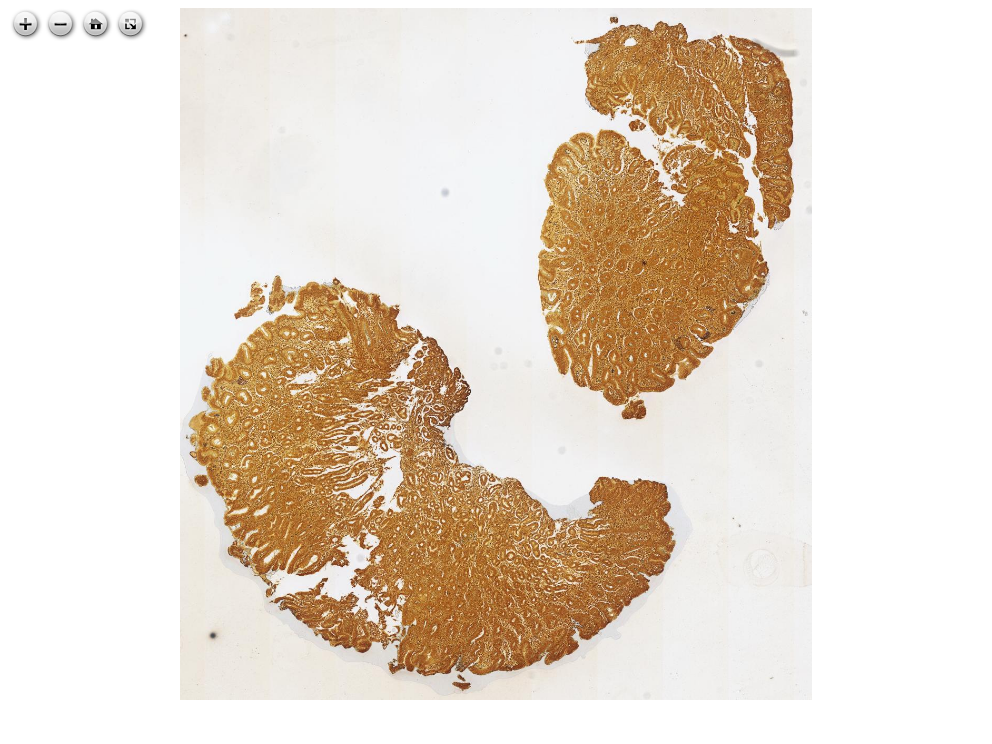
\includegraphics[width=0.25\textwidth,height=\textheight]{./screenshots/thumbnail_helicobacterpyloriWS.png}}
\href{https://images.patolojiatlasi.com/helicobacterpylori/warthinstarry.html}{Tam
Ekran Görmek İçin Resmi Tıklayın}

\hypertarget{giemsa}{%
\subsection{Giemsa}\label{giemsa}}

\textbf{Mide'de Helicobacter pylori (H. pylori) Giemsa Histokimyası}

\href{https://images.patolojiatlasi.com/helicobacterpylori/giemsa.html}{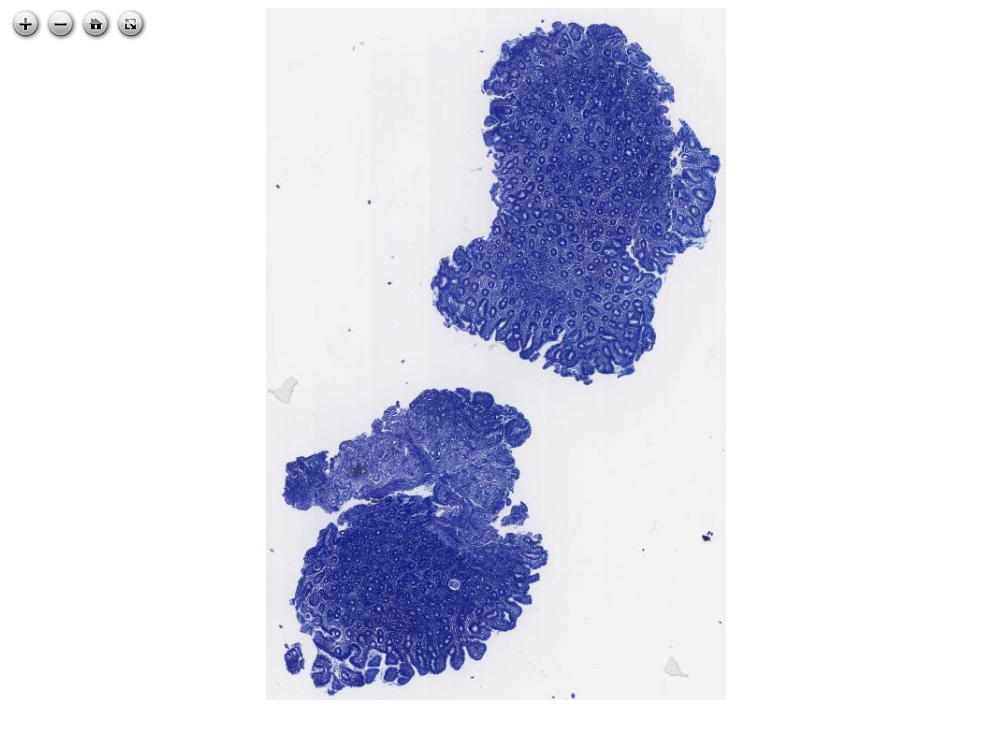
\includegraphics[width=0.25\textwidth,height=\textheight]{./screenshots/thumbnail_helicobacterpyloriGiemsa.png}}
\href{https://images.patolojiatlasi.com/helicobacterpylori/giemsa.html}{Tam
Ekran Görmek İçin Resmi Tıklayın}

\hypertarget{ihc}{%
\subsection{IHC}\label{ihc}}

\textbf{Mide'de Helicobacter pylori (H. pylori) İmmünohistokimyası}

\href{https://images.patolojiatlasi.com/helicobacterpylori/IHC.html}{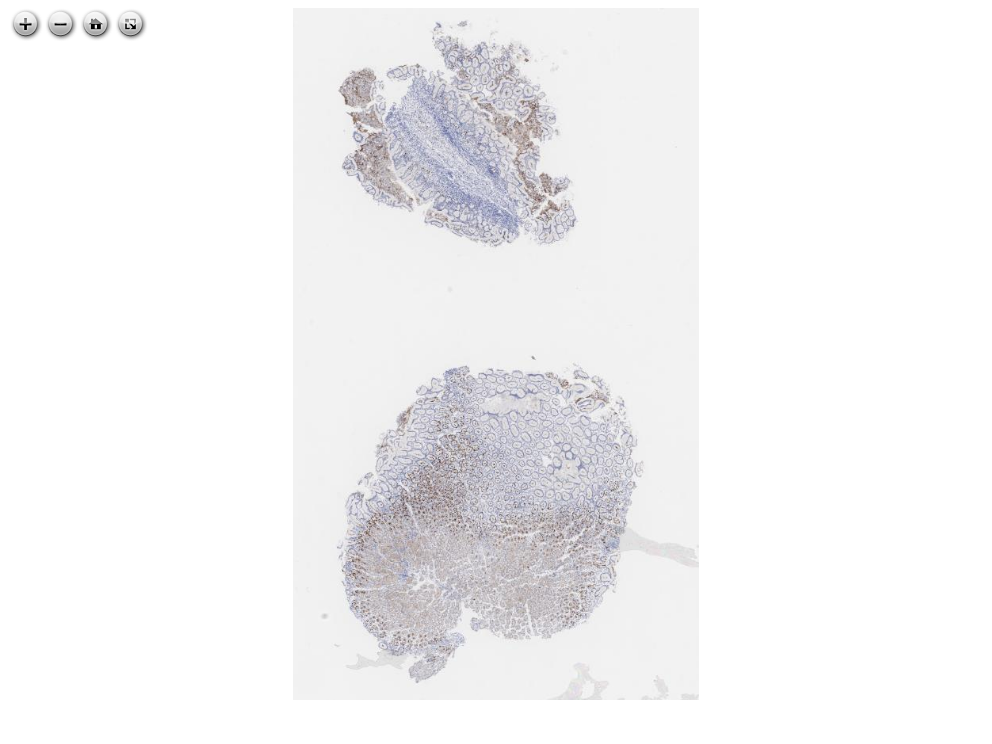
\includegraphics[width=0.25\textwidth,height=\textheight]{./screenshots/thumbnail_helicobacterpyloriIHC.png}}
\href{https://images.patolojiatlasi.com/helicobacterpylori/IHC.html}{Tam
Ekran Görmek İçin Resmi Tıklayın}

\hypertarget{sec-mantarlar}{%
\chapter{Mantarlar}\label{sec-mantarlar}}

\hypertarget{sec-candida-albicans-in-cervicovaginal-smear}{%
\section{\texorpdfstring{Candida \emph{albicans} in cervicovaginal
smear}{Candida albicans in cervicovaginal smear}}\label{sec-candida-albicans-in-cervicovaginal-smear}}

\href{https://images.patolojiatlasi.com/candidaalbicans/cervicovaginalsmear/viewer_z0.html}{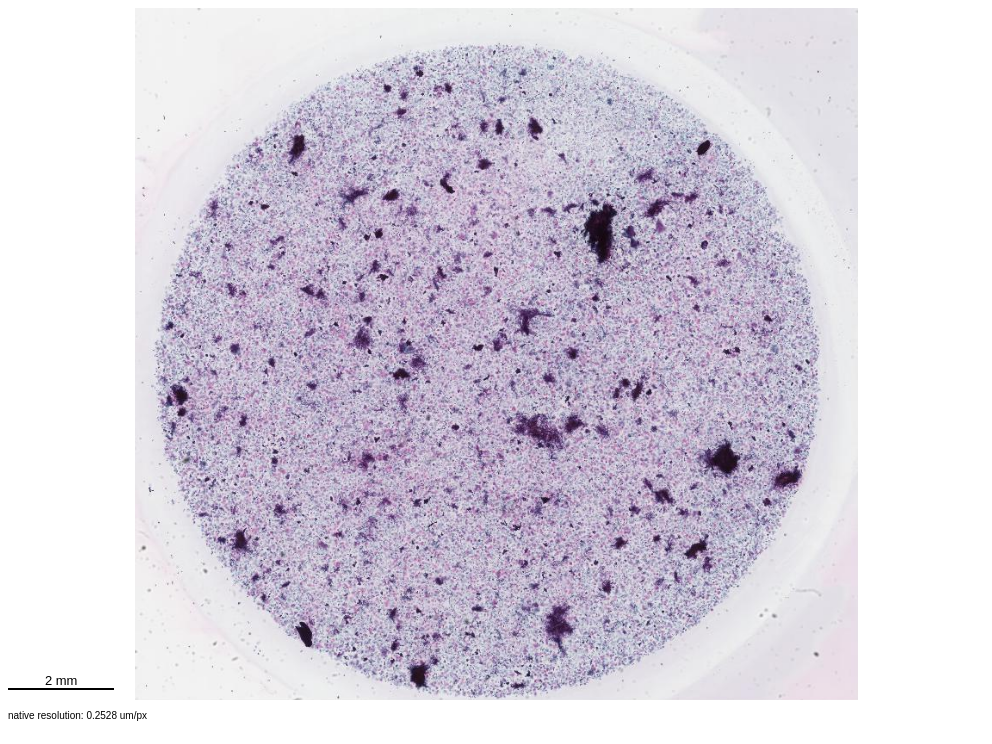
\includegraphics[width=0.25\textwidth,height=\textheight]{./screenshots/thumbnail_candidaalbicans.png}}
\href{https://images.patolojiatlasi.com/candidaalbicans/cervicovaginalsmear/viewer_z0.html}{Tam
Ekran Görmek İçin Resmi Tıklayın}

\hypertarget{sec-beyin-mukormikozis}{%
\section{Beyin mukormikozis}\label{sec-beyin-mukormikozis}}

\hypertarget{he-5}{%
\subsection{HE}\label{he-5}}

\textbf{Beyin mukormikozis HE}

\href{https://images.patolojiatlasi.com/brain-mucormycosis/HE.html}{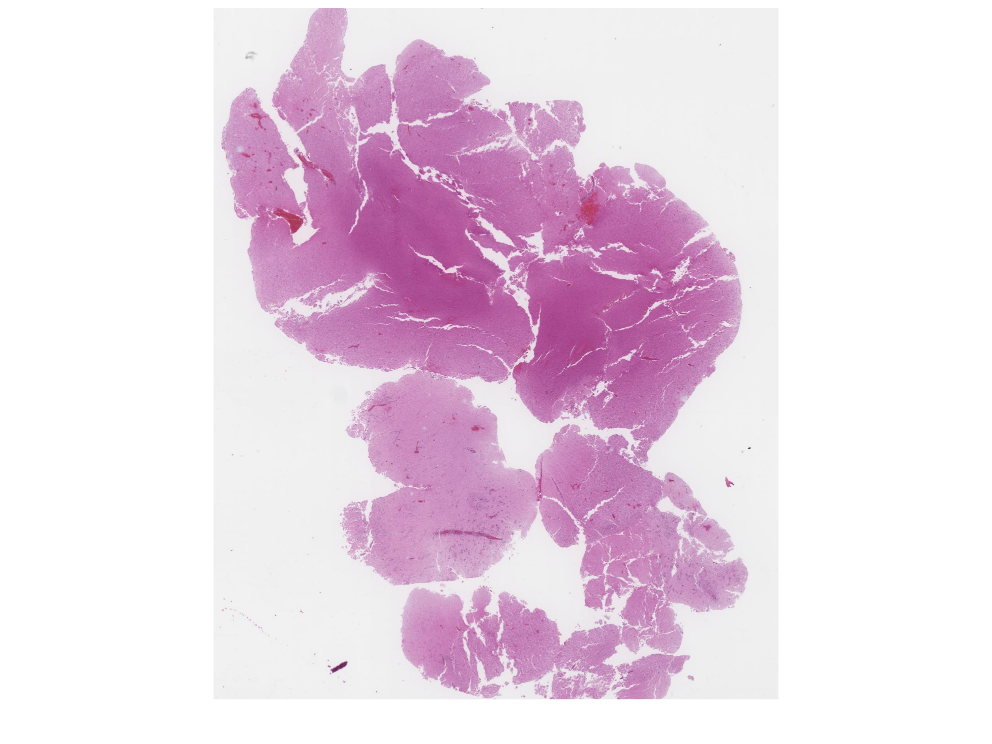
\includegraphics[width=0.25\textwidth,height=\textheight]{./screenshots/thumbnail_brain-mucormycosis.png}}
\href{https://images.patolojiatlasi.com/brain-mucormycosis/HE.html}{Tam
Ekran Görmek İçin Resmi Tıklayın}

\hypertarget{gms}{%
\subsection{GMS}\label{gms}}

\textbf{Beyin mukormikozis GMS}

\href{https://images.patolojiatlasi.com/brain-mucormycosis/GMS.html}{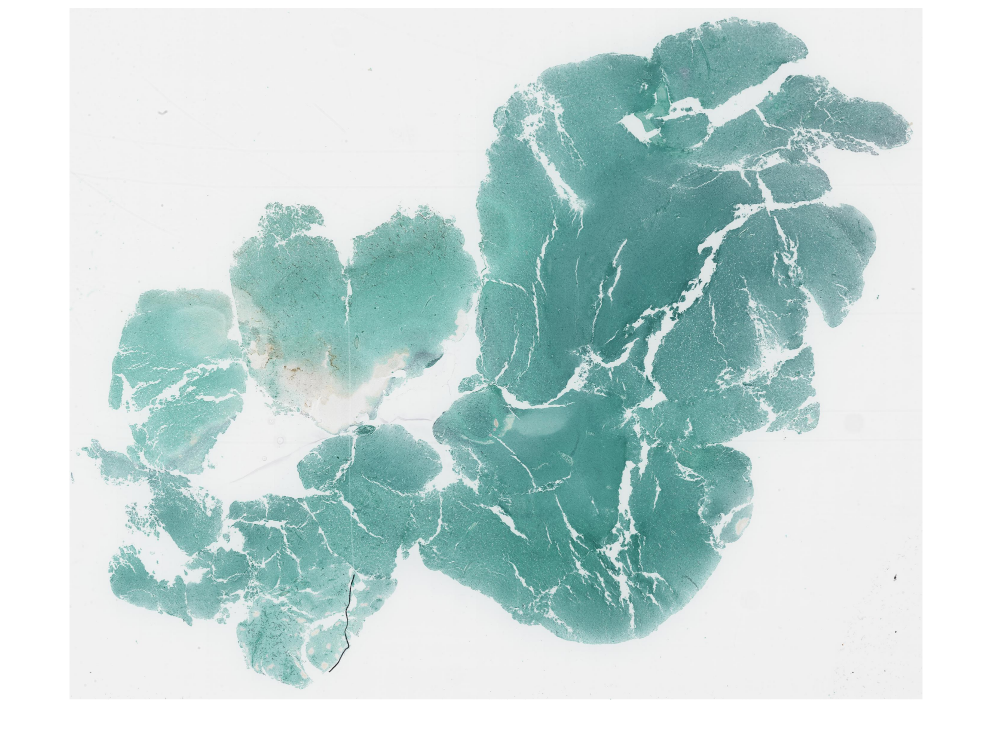
\includegraphics[width=0.25\textwidth,height=\textheight]{./screenshots/thumbnail_brain-mucormycosis-GMS.png}}
\href{https://images.patolojiatlasi.com/brain-mucormycosis/GMS.html}{Tam
Ekran Görmek İçin Resmi Tıklayın}

\hypertarget{sec-parazitler}{%
\chapter{Parazitler}\label{sec-parazitler}}

\hypertarget{sec-enterobius-vermicularis}{%
\section{Enterobius vermicularis}\label{sec-enterobius-vermicularis}}

\textbf{Enterobius vermicularis}

\href{https://images.patolojiatlasi.com/enterobius-vermicularis/HE.html}{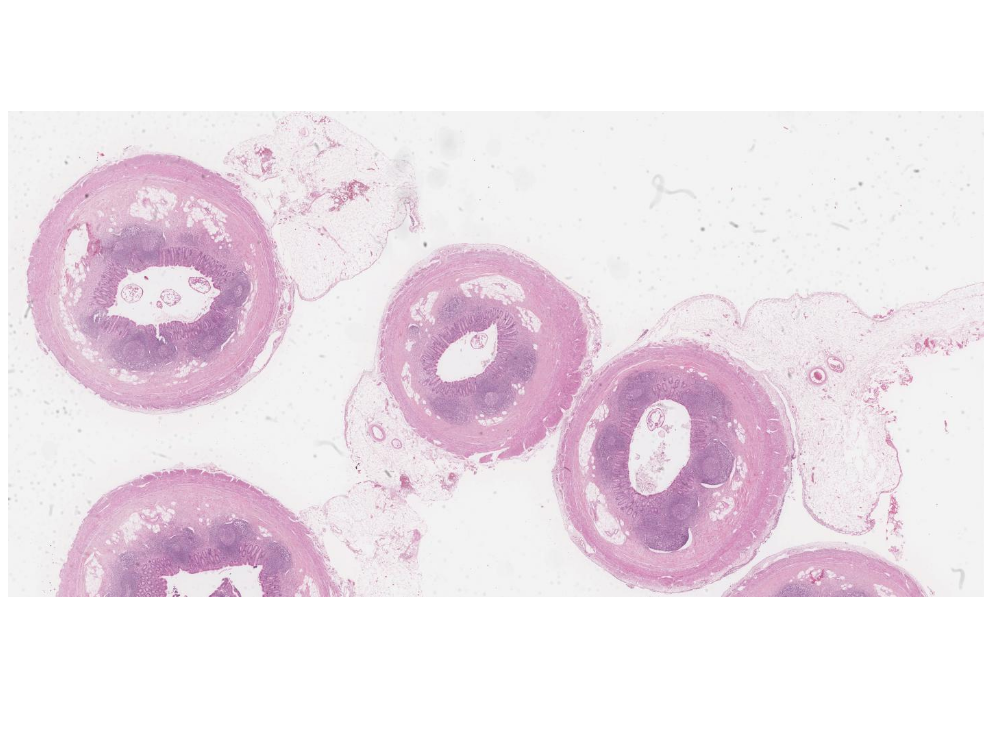
\includegraphics[width=0.25\textwidth,height=\textheight]{./screenshots/thumbnail_enterobius-vermicularis.png}}
\href{https://images.patolojiatlasi.com/enterobius-vermicularis/HE.html}{Tam
Ekran Görmek İçin Resmi Tıklayın}

\part{Temel Tümör Patolojisi}

\hypertarget{sec-benign-tumorler}{%
\chapter{Benign Tümörler}\label{sec-benign-tumorler}}

\hypertarget{sec-adenomlar}{%
\section{Adenomlar}\label{sec-adenomlar}}

\hypertarget{sec-tubuler-adenom}{%
\subsection{Tübüler Adenom}\label{sec-tubuler-adenom}}

\hypertarget{sec-sesil-polip}{%
\subsubsection{Sesil Polip, Flat (Düz) Tübüler
Adenom}\label{sec-sesil-polip}}

\href{https://images.patolojiatlasi.com/tubularadenoma-flat/HE.html}{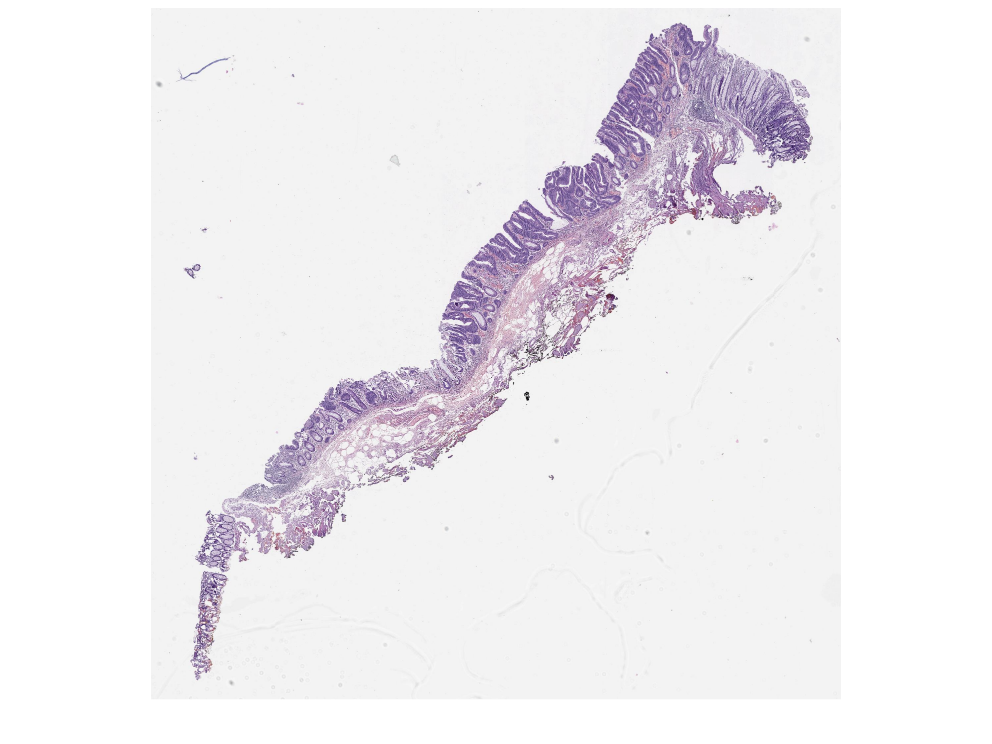
\includegraphics[width=0.25\textwidth,height=\textheight]{./screenshots/thumbnail_tubularadenoma-flat1.png}}
\href{https://images.patolojiatlasi.com/tubularadenoma-flat/HE.html}{Tam
Ekran Görmek İçin Resmi Tıklayın}

\href{https://images.patolojiatlasi.com/tubularadenoma-flat/HE2.html}{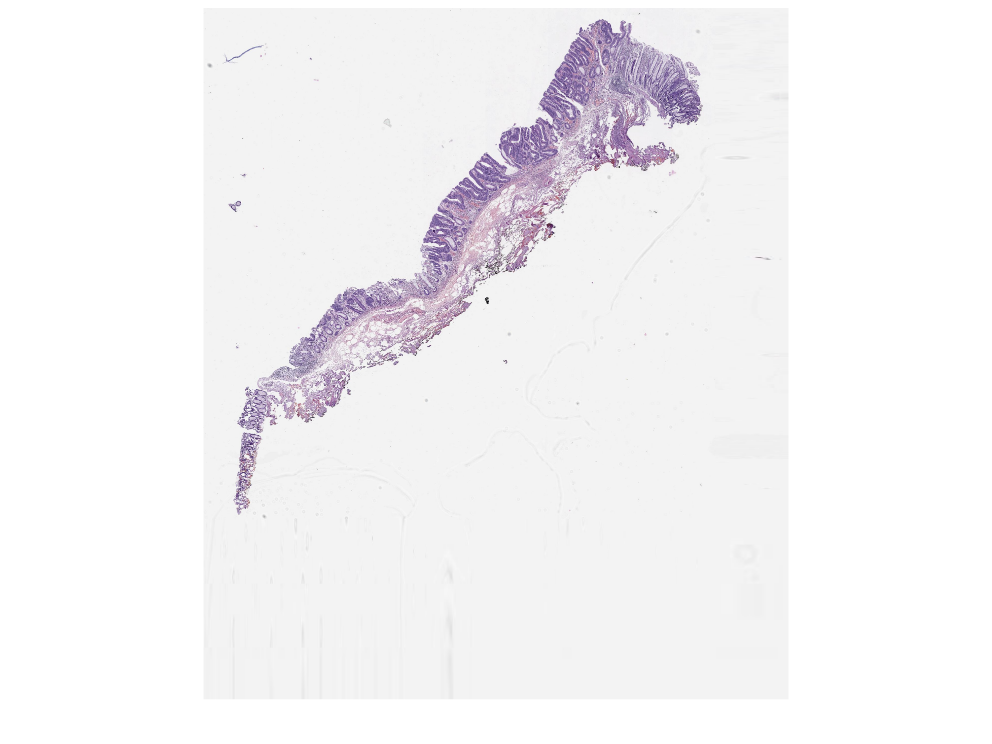
\includegraphics[width=0.25\textwidth,height=\textheight]{./screenshots/thumbnail_tubularadenoma-flat2.png}}
\href{https://images.patolojiatlasi.com/tubularadenoma-flat/HE2.html}{Tam
Ekran Görmek İçin Resmi Tıklayın}

\hypertarget{sec-sapli-polip}{%
\subsubsection{Saplı Polip}\label{sec-sapli-polip}}

\hypertarget{macroscopy}{%
\subsection{Macroscopy}\label{macroscopy}}

\href{https://images.patolojiatlasi.com/tubularadenoma/tubular-adenoma-with-stalk-macroscopy.png}{tubular
adenoma with a stalk macroscopy}

\hypertarget{mikroskopi}{%
\subsection{Mikroskopi}\label{mikroskopi}}

Mikroskopi

\href{https://images.patolojiatlasi.com/tubularadenoma/tubular-adenoma-with-stalk.png}{tubular
adenoma with a stalk}

\href{https://images.patolojiatlasi.com/tubularadenoma/tubular-adenoma-with-stalk/viewer_z0.html}{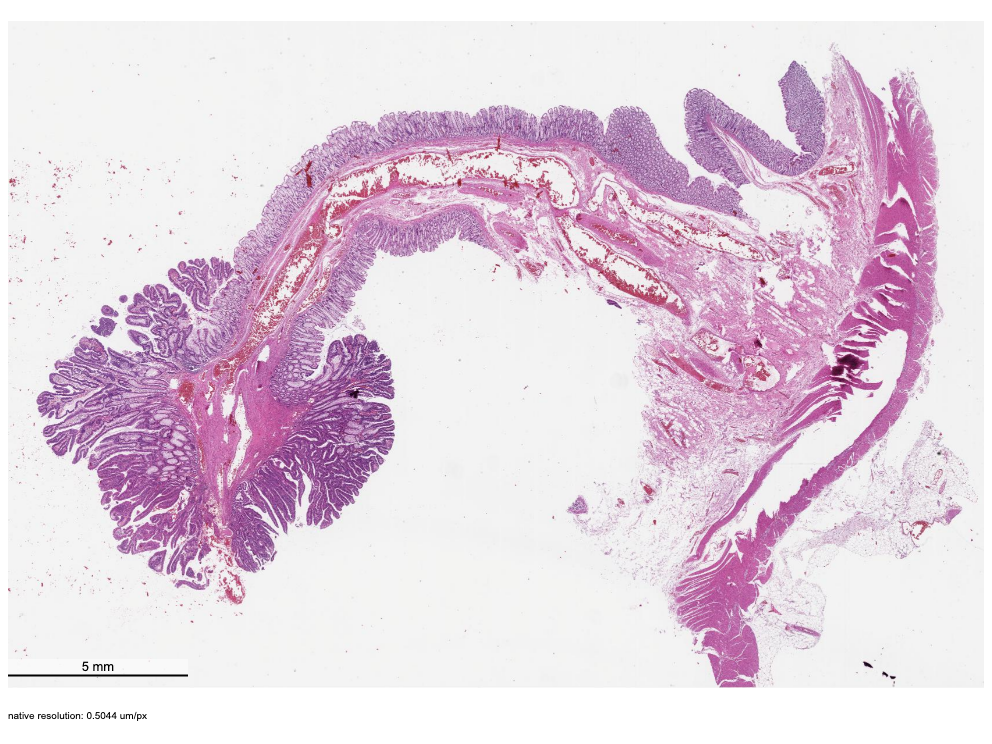
\includegraphics[width=0.25\textwidth,height=\textheight]{./screenshots/thumbnail_tubular-adenoma-with-stalk.png}}
\href{https://images.patolojiatlasi.com/tubularadenoma/tubular-adenoma-with-stalk/viewer_z0.html}{Tam
Ekran Görmek İçin Resmi Tıklayın}

\hypertarget{sec-hamartom}{%
\chapter{Hamartom}\label{sec-hamartom}}

\hypertarget{sec-hamartomatoz-polip}{%
\section{Hamartomatöz Polip}\label{sec-hamartomatoz-polip}}

\href{https://images.patolojiatlasi.com/hamartomatouspolyp/HE.html}{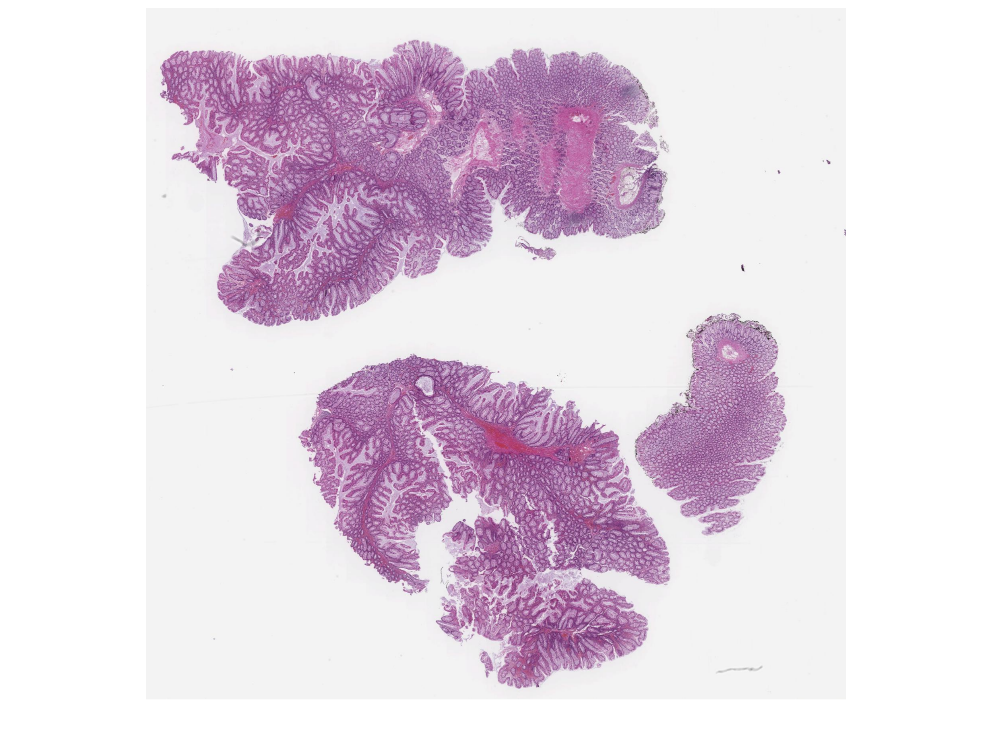
\includegraphics[width=0.25\textwidth,height=\textheight]{./screenshots/thumbnail_hamartomatouspolyp.png}}
\href{https://images.patolojiatlasi.com/hamartomatouspolyp/HE.html}{Tam
Ekran Görmek İçin Resmi Tıklayın}

\hypertarget{sec-schwann-cell-hamartoma-colon-polyp}{%
\section{Schwann Cell Hamartoma in a Colon
Polyp}\label{sec-schwann-cell-hamartoma-colon-polyp}}

\href{https://images.patolojiatlasi.com/schwanncellhamartoma/HE.html}{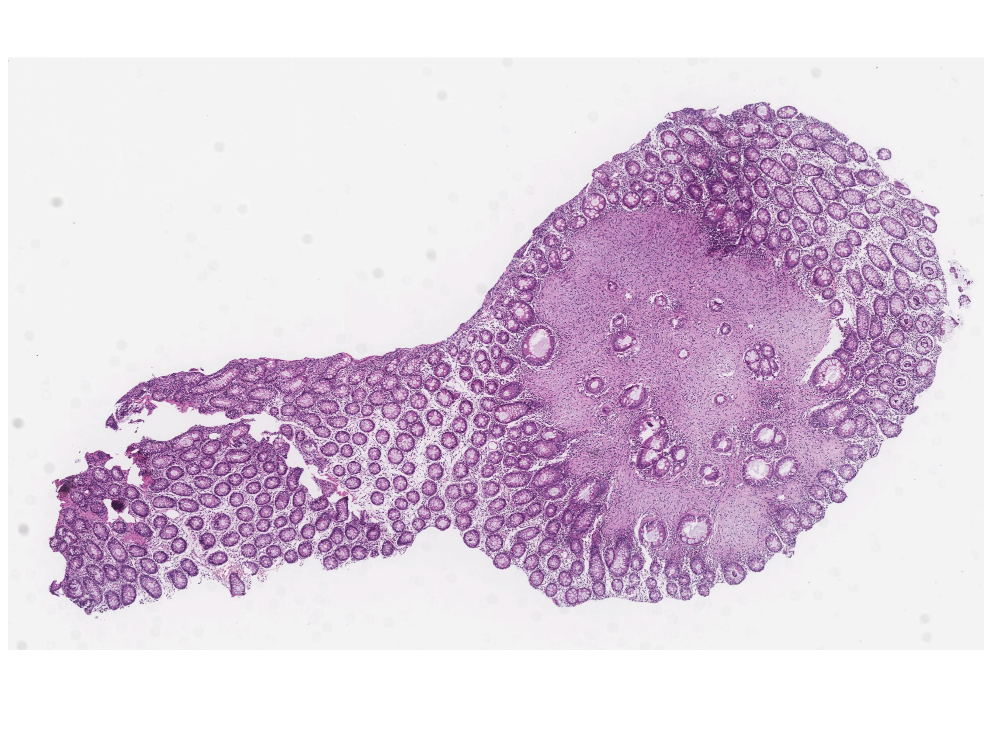
\includegraphics[width=0.25\textwidth,height=\textheight]{./screenshots/thumbnail_schwanncellhamartoma.png}}
\href{https://images.patolojiatlasi.com/schwanncellhamartoma/HE.html}{Tam
Ekran Görmek İçin Resmi Tıklayın}

\hypertarget{sec-heterotopi-ektopi}{%
\chapter{Heterotopi Ektopi}\label{sec-heterotopi-ektopi}}

\hypertarget{sec-intrapancreatic-spleen}{%
\section{Intrapancreatic Spleen,
Heterotopia}\label{sec-intrapancreatic-spleen}}

\href{https://images.patolojiatlasi.com/intrapancreaticspleen/HE.html}{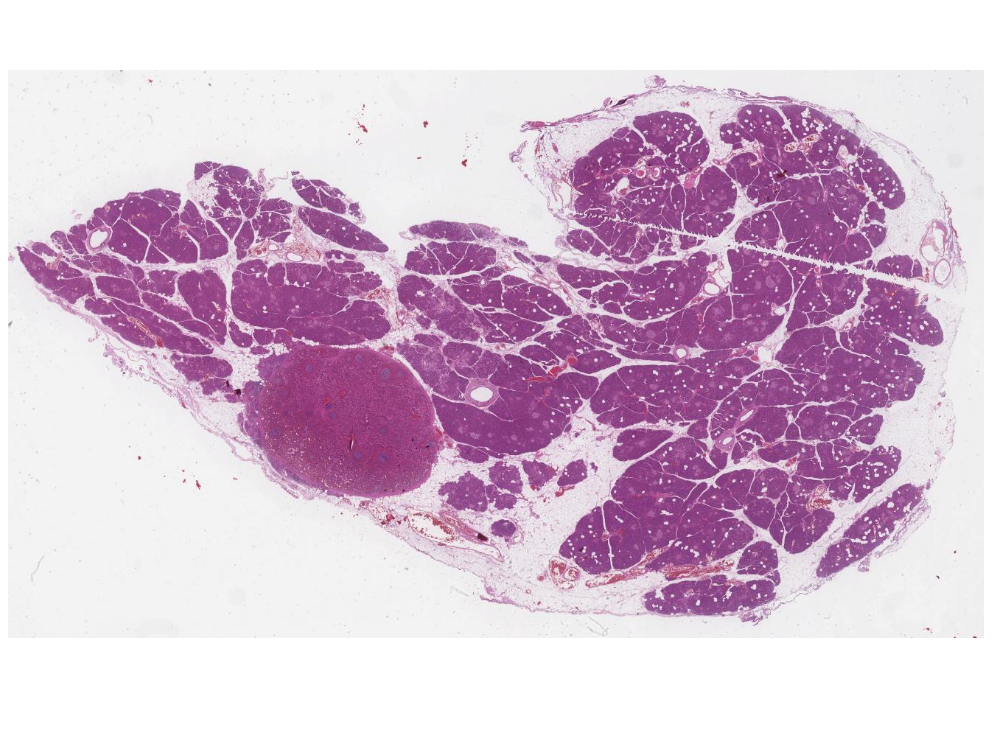
\includegraphics[width=0.25\textwidth,height=\textheight]{./screenshots/thumbnail_intrapancreaticspleen.png}}
\href{https://images.patolojiatlasi.com/intrapancreaticspleen/HE.html}{Tam
Ekran Görmek İçin Resmi Tıklayın}

\hypertarget{sec-paratubal-adneksiyal-bolgede-ektopik-adrenal}{%
\section{Paratubal adneksiyal bölgede ektopik adrenal
dokusu}\label{sec-paratubal-adneksiyal-bolgede-ektopik-adrenal}}

\textbf{Paratubal adneksiyal bölgede ektopik adrenal dokusu}

\href{https://images.patolojiatlasi.com/ectopic-adrenal/HE.html}{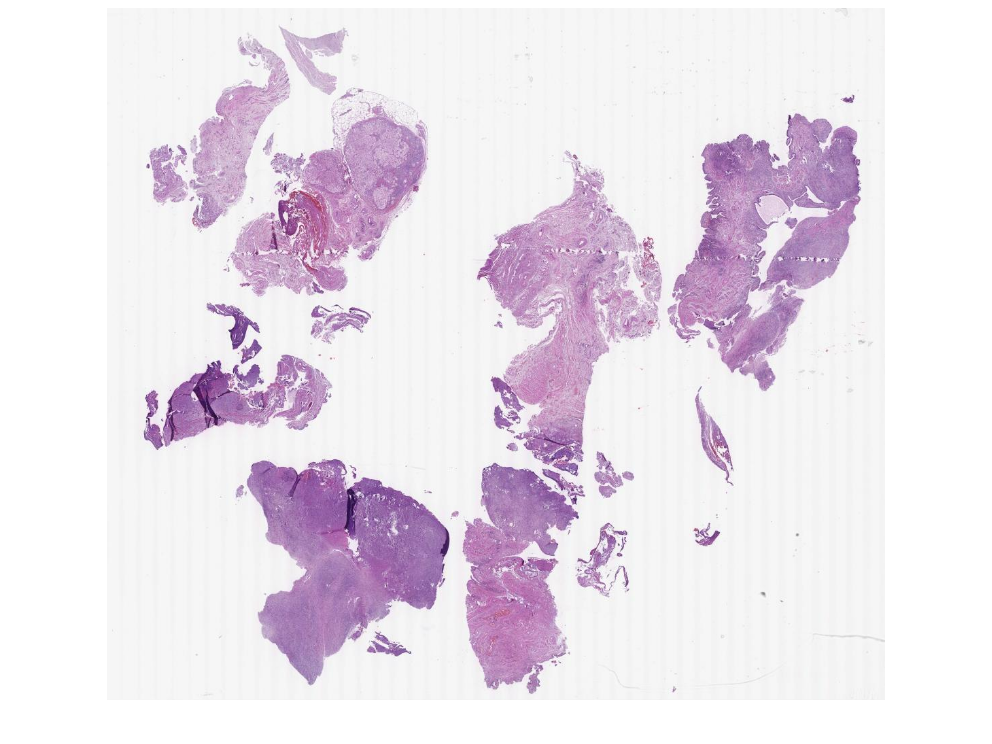
\includegraphics[width=0.25\textwidth,height=\textheight]{./screenshots/thumbnail_ectopic-adrenal.png}}
\href{https://images.patolojiatlasi.com/ectopic-adrenal/HE.html}{Tam
Ekran Görmek İçin Resmi Tıklayın}

\hypertarget{sec-metaplazi}{%
\chapter{Metaplazi}\label{sec-metaplazi}}

\hypertarget{sec-pankreatik-asiner-metaplazi}{%
\section{Pankreatik Asiner Metaplazi,
Mide}\label{sec-pankreatik-asiner-metaplazi}}

\hypertarget{he-6}{%
\subsection{HE}\label{he-6}}

\textbf{Pankreatik Asiner Metaplazi, Mide}

\href{https://images.patolojiatlasi.com/metaplasia/HE.html}{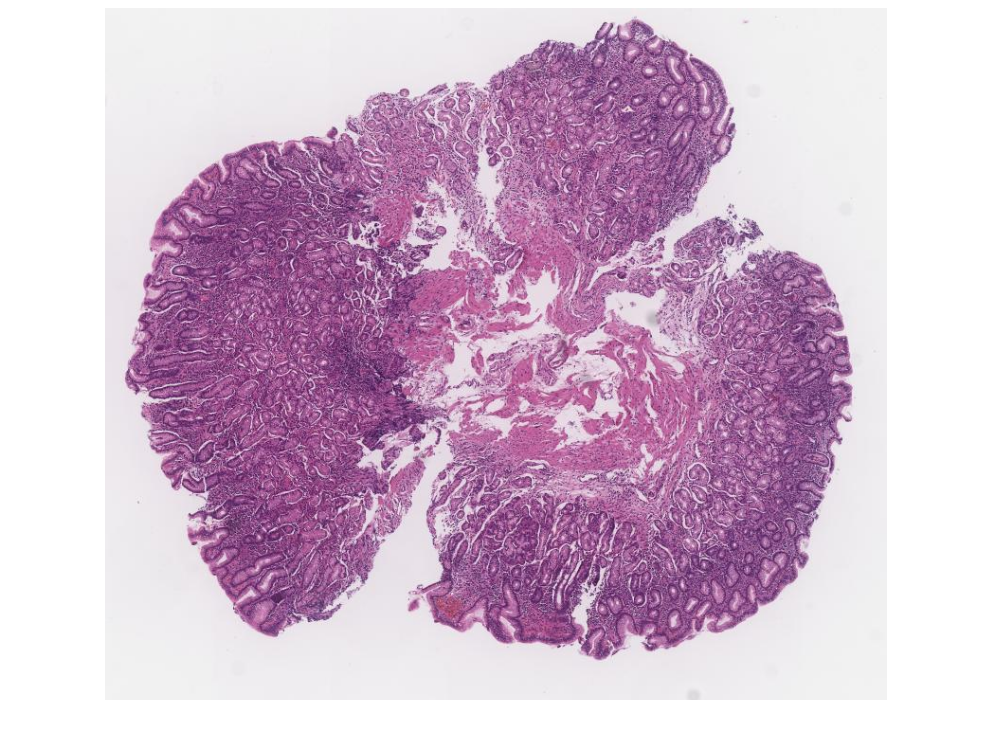
\includegraphics[width=0.25\textwidth,height=\textheight]{./screenshots/thumbnail_metaplasia.png}}
\href{https://images.patolojiatlasi.com/metaplasia/HE.html}{Tam Ekran
Görmek İçin Resmi Tıklayın}

\hypertarget{he---annotated}{%
\subsection{HE - annotated}\label{he---annotated}}

\href{https://images.patolojiatlasi.com/metaplasia/HE_annotated.html}{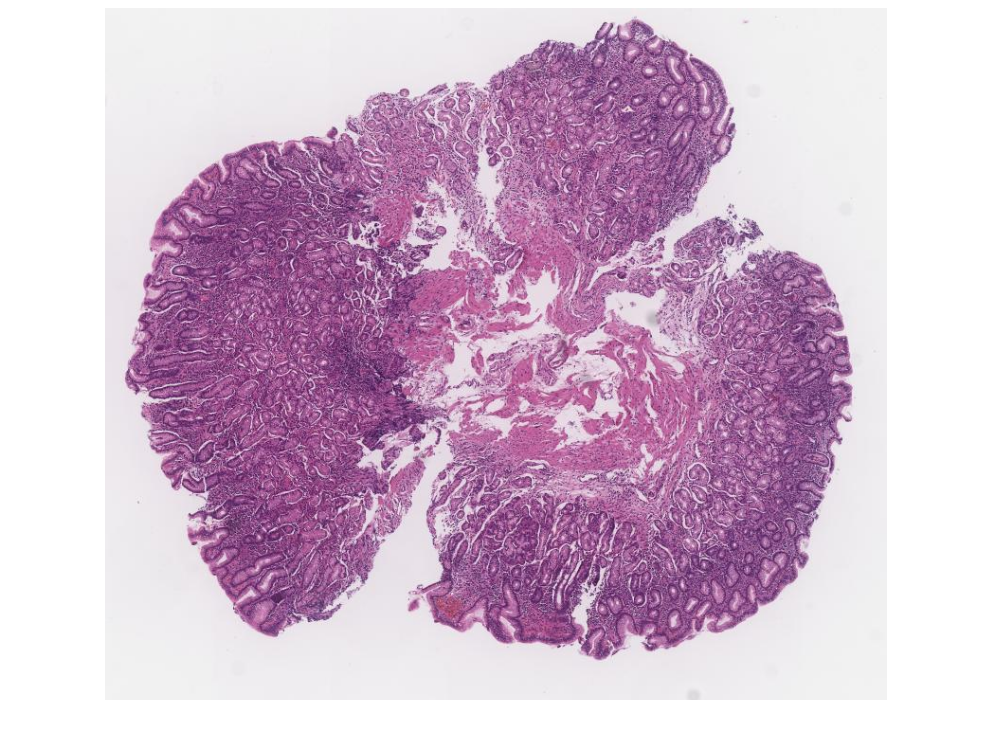
\includegraphics[width=0.25\textwidth,height=\textheight]{./screenshots/thumbnail_metaplasia.png}}
\href{https://images.patolojiatlasi.com/metaplasia/HE_annotated.html}{Tam
Ekran Görmek İçin Resmi Tıklayın}

\hypertarget{trypsin}{%
\subsection{Trypsin}\label{trypsin}}

\href{https://images.patolojiatlasi.com/metaplasia/trypsin.html}{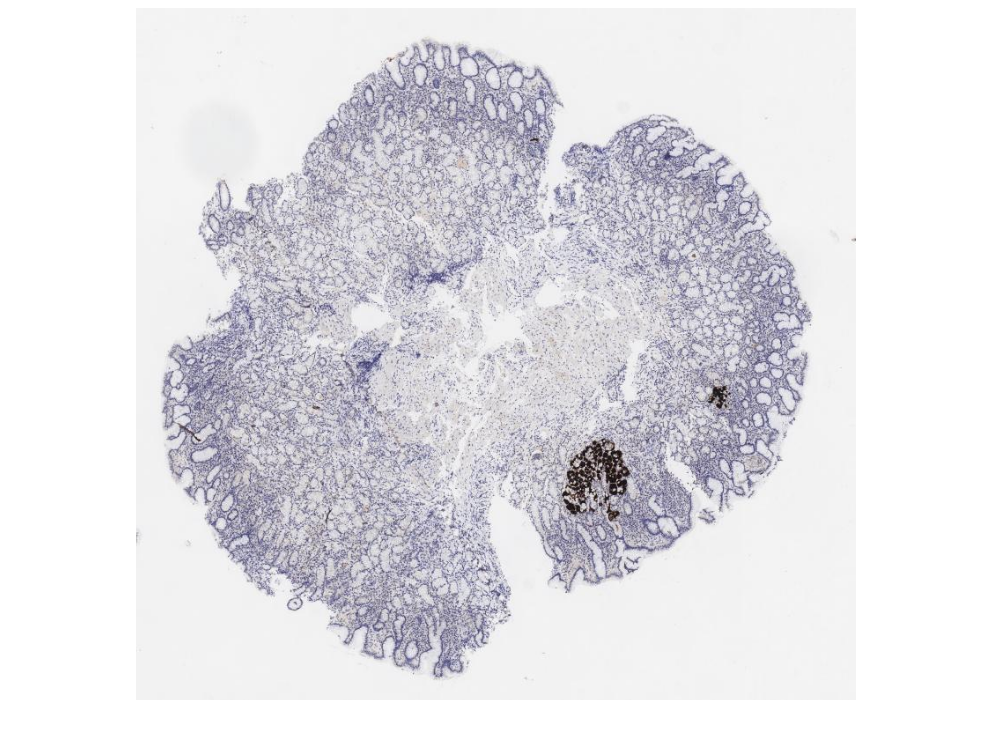
\includegraphics[width=0.25\textwidth,height=\textheight]{./screenshots/thumbnail_metaplasia-trypsin.png}}
\href{https://images.patolojiatlasi.com/metaplasia/trypsin.html}{Tam
Ekran Görmek İçin Resmi Tıklayın}

\hypertarget{sec-karsinogenez}{%
\chapter{Karsinogenez}\label{sec-karsinogenez}}

\hypertarget{sec-mepaplazi-displazi-karsinom}{%
\section{metaplazi, displazi,
karsinom}\label{sec-mepaplazi-displazi-karsinom}}

\textbf{metaplazi, displazi, karsinom}

\href{https://images.patolojiatlasi.com/carcinogenesis/HE.html}{\includegraphics[width=0.25\textwidth,height=\textheight]{./screenshots/thumbnail_carcinogenesis.png}}
\href{https://images.patolojiatlasi.com/carcinogenesis/HE.html}{Tam
Ekran Görmek İçin Resmi Tıklayın}

\hypertarget{sec-malign-tumor-ozellikleri}{%
\chapter{Malign Tümör Özellikleri}\label{sec-malign-tumor-ozellikleri}}

\hypertarget{sec-pleomorfizm}{%
\section{Pleomorfizm}\label{sec-pleomorfizm}}

\textbf{Pleomorfizm}

\href{https://images.patolojiatlasi.com/pleomorphism/HE.html}{\includegraphics[width=0.25\textwidth,height=\textheight]{./screenshots/thumbnail_pleomorphism.png}}
\href{https://images.patolojiatlasi.com/pleomorphism/HE.html}{Tam Ekran
Görmek İçin Resmi Tıklayın}

\hypertarget{sec-metastaz}{%
\chapter{Metastaz}\label{sec-metastaz}}

\hypertarget{sec-karaciger-sarkom-metastaz}{%
\section{Karaciğerde Sarkom
Metastazı}\label{sec-karaciger-sarkom-metastaz}}

\href{https://images.patolojiatlasi.com/metastaticsarcoma/HE.html}{\includegraphics[width=0.25\textwidth,height=\textheight]{./screenshots/thumbnail_metastaticsarcoma.png}}
\href{https://images.patolojiatlasi.com/metastaticsarcoma/HE.html}{Tam
Ekran Görmek İçin Resmi Tıklayın}

\hypertarget{sec-sinsi-lenf-nodu-metastazi}{%
\section{Sinsi bir lenf nodu
metastazı}\label{sec-sinsi-lenf-nodu-metastazi}}

\hypertarget{he-7}{%
\subsection{HE}\label{he-7}}

\textbf{Sinsi bir lenf nodu metastazı HE}

\href{https://images.patolojiatlasi.com/insidious-lymph-node-metastasis/HE.html}{\includegraphics[width=0.25\textwidth,height=\textheight]{./screenshots/thumbnail_insidious-lymph-node-metastasis.png}}
\href{https://images.patolojiatlasi.com/insidious-lymph-node-metastasis/HE.html}{Tam
Ekran Görmek İçin Resmi Tıklayın}

\hypertarget{ihc-1}{%
\subsection{IHC}\label{ihc-1}}

\textbf{Sinsi bir lenf nodu metastazı OSKAR panCK}

\href{https://images.patolojiatlasi.com/insidious-lymph-node-metastasis/HE.html}{\includegraphics[width=0.25\textwidth,height=\textheight]{./screenshots/thumbnail_insidious-lymph-node-metastasis-OSKARCK.png}}
\href{https://images.patolojiatlasi.com/insidious-lymph-node-metastasis/OSKARCK.html}{Tam
Ekran Görmek İçin Resmi Tıklayın}

\hypertarget{sec-baska-organlara-tumor-yayilimi}{%
\chapter{Başka Organlara Tümör
Yayılımı}\label{sec-baska-organlara-tumor-yayilimi}}

\hypertarget{sec-servikse-kolon-tumor-yayilimi}{%
\section{Servikse kolon tümörü
yayılımı}\label{sec-servikse-kolon-tumor-yayilimi}}

\textbf{Servikse kolon tümörü yayılımı}

\href{https://images.patolojiatlasi.com/tumor-spread/HE-cervix.html}{\includegraphics[width=0.25\textwidth,height=\textheight]{./screenshots/thumbnail_tumor-spread-cervix.png}}
\href{https://images.patolojiatlasi.com/tumor-spread/HE-cervix.html}{Tam
Ekran Görmek İçin Resmi Tıklayın}

\hypertarget{sec-endometriuma-kolon-tumor-yayilimi}{%
\section{Endometriuma kolon tümörü
yayılımı}\label{sec-endometriuma-kolon-tumor-yayilimi}}

\textbf{Endometriuma kolon tümörü yayılımı}

\href{https://images.patolojiatlasi.com/tumor-spread/HE-endometrium.html}{\includegraphics[width=0.25\textwidth,height=\textheight]{./screenshots/thumbnail_tumor-spread-endometrium.png}}
\href{https://images.patolojiatlasi.com/tumor-spread/HE-endometrium.html}{Tam
Ekran Görmek İçin Resmi Tıklayın}

\hypertarget{sec-overe-kolon-tumor-yayilimi}{%
\section{Overe kolon tümörü
yayılımı}\label{sec-overe-kolon-tumor-yayilimi}}

\textbf{Overe kolon tümörü yayılımı}

\href{https://images.patolojiatlasi.com/tumor-spread/HE-over.html}{\includegraphics[width=0.25\textwidth,height=\textheight]{./screenshots/thumbnail_tumor-spread-over.png}}
\href{https://images.patolojiatlasi.com/tumor-spread/HE-over.html}{Tam
Ekran Görmek İçin Resmi Tıklayın}

\hypertarget{sec-ince-barsak-kolon-tumor-yayilimi}{%
\section{İnce barsağa kolon tümörü
yayılımı}\label{sec-ince-barsak-kolon-tumor-yayilimi}}

\textbf{İnce barsağa kolon tümörü yayılımı}

\href{https://images.patolojiatlasi.com/tumor-spread/HE-small-intestine.html}{\includegraphics[width=0.25\textwidth,height=\textheight]{./screenshots/thumbnail_tumor-spread-small-intestine.png}}
\href{https://images.patolojiatlasi.com/tumor-spread/HE-small-intestine.html}{Tam
Ekran Görmek İçin Resmi Tıklayın}

\part{Tümörlerdeki Prognostik Morfolojik Özellikler}

\hypertarget{sec-venoz-invazyon}{%
\chapter{Venöz invazyon}\label{sec-venoz-invazyon}}

\textbf{Venöz invazyon}

\href{https://images.patolojiatlasi.com/venous-invasion/HE.html}{\includegraphics[width=0.25\textwidth,height=\textheight]{./screenshots/thumbnail_venous-invasion.png}}
\href{https://images.patolojiatlasi.com/venous-invasion/HE.html}{Tam
Ekran Görmek İçin Resmi Tıklayın}

\hypertarget{sec-ekstramural-venoz-invazyon}{%
\chapter{Ekstramural Venöz
İnvazyon}\label{sec-ekstramural-venoz-invazyon}}

\hypertarget{sec-adenokarsinomda-ekstramural-venoz-invazyon}{%
\chapter{Adenokarsinomda Ekstramural Venöz
İnvazyon}\label{sec-adenokarsinomda-ekstramural-venoz-invazyon}}

\textbf{Adenokarsinomda Ekstramural Venöz İnvazyon}

\href{https://images.patolojiatlasi.com/extramuralvenousinvasion/HE.html}{\includegraphics[width=0.25\textwidth,height=\textheight]{./screenshots/thumbnail_extramuralvenousinvasion.png}}
\href{https://images.patolojiatlasi.com/extramuralvenousinvasion/HE.html}{Tam
Ekran Görmek İçin Resmi Tıklayın}

\href{https://images.patolojiatlasi.com/extramuralvenousinvasion/HE2.html}{\includegraphics[width=0.25\textwidth,height=\textheight]{./screenshots/thumbnail_extramuralvenousinvasion-2.png}}
\href{https://images.patolojiatlasi.com/extramuralvenousinvasion/HE2.html}{Tam
Ekran Görmek İçin Resmi Tıklayın}

\textbf{ekstramural venöz invazyon}

\href{https://images.patolojiatlasi.com/extramural-venous-invasion/HE.html}{\includegraphics[width=0.25\textwidth,height=\textheight]{./screenshots/thumbnail_extramural-venous-invasion.png}}
\href{https://images.patolojiatlasi.com/extramural-venous-invasion/HE.html}{Tam
Ekran Görmek İçin Resmi Tıklayın}

\part{Hematopatoloji}

\hypertarget{sec-hodgkin-lenfoma}{%
\chapter{Hodgkin Lenfoma}\label{sec-hodgkin-lenfoma}}

\textbf{Hodgkin Lenfoma}

\href{https://images.patolojiatlasi.com/hodgkin/HE.html}{\includegraphics[width=0.25\textwidth,height=\textheight]{./screenshots/thumbnail_hodgkin.png}}
\href{https://images.patolojiatlasi.com/hodgkin/HE.html}{Tam Ekran
Görmek İçin Resmi Tıklayın}

\part{Gastrointestinal Sistem Patolojisi}

\hypertarget{sec-gastrointestinal-sistem}{%
\chapter{Gastrointestinal Sistem}\label{sec-gastrointestinal-sistem}}

\hypertarget{sec-ozofagus}{%
\chapter{Özofagus}\label{sec-ozofagus}}

\hypertarget{sec-ozofagus-granuler-hucreli-tumor}{%
\section{Özofagusta Granüler Hücreli
Tümör}\label{sec-ozofagus-granuler-hucreli-tumor}}

\textbf{Özofagusta Granüler Hücreli Tümör}

\href{https://images.patolojiatlasi.com/granular-cell-tumor/HE.html}{\includegraphics[width=0.25\textwidth,height=\textheight]{./screenshots/thumbnail_granular-cell-tumor.png}}
\href{https://images.patolojiatlasi.com/granular-cell-tumor/HE.html}{Tam
Ekran Görmek İçin Resmi Tıklayın}

\hypertarget{sec-mide-patolojisi}{%
\chapter{Mide Patolojisi}\label{sec-mide-patolojisi}}

\hypertarget{sec-gastritis-cystica-profunda}{%
\section{Gastritis Cystica
Profunda}\label{sec-gastritis-cystica-profunda}}

\textbf{Gastritis Cystica Profunda}

\href{https://images.patolojiatlasi.com/gastritis-cystica-profunda/HE.html}{\includegraphics[width=0.25\textwidth,height=\textheight]{./screenshots/thumbnail_gastritis-cystica-profunda.png}}
\href{https://images.patolojiatlasi.com/gastritis-cystica-profunda/HE.html}{Tam
Ekran Görmek İçin Resmi Tıklayın}

\hypertarget{sec-gastrit}{%
\chapter{Gastrit}\label{sec-gastrit}}

\hypertarget{sec-lymphocytic-gastritis}{%
\section{lenfositik gastrit}\label{sec-lymphocytic-gastritis}}

\textbf{lenfositik gastrit}

\href{https://images.patolojiatlasi.com/lymphocytic-gastritis/all.html}{\includegraphics[width=0.25\textwidth,height=\textheight]{./screenshots/thumbnail_lymphocytic-gastritis-all.png}}
\href{https://images.patolojiatlasi.com/lymphocytic-gastritis/all.html}{Tam
Ekran Görmek İçin Resmi Tıklayın}

\hypertarget{he-8}{%
\subsection{HE}\label{he-8}}

\textbf{lenfositik gastrit HE}

\href{https://images.patolojiatlasi.com/lymphocytic-gastritis/HE.html}{\includegraphics[width=0.25\textwidth,height=\textheight]{./screenshots/thumbnail_lymphocytic-gastritisHE.png}}
\href{https://images.patolojiatlasi.com/lymphocytic-gastritis/HE.html}{Tam
Ekran Görmek İçin Resmi Tıklayın}

\hypertarget{cd3}{%
\subsection{CD3}\label{cd3}}

\textbf{lenfositik gastrit CD3}

\href{https://images.patolojiatlasi.com/lymphocytic-gastritis/CD3.html}{\includegraphics[width=0.25\textwidth,height=\textheight]{./screenshots/thumbnail_lymphocytic-gastritisCD3.png}}
\href{https://images.patolojiatlasi.com/lymphocytic-gastritis/CD3.html}{Tam
Ekran Görmek İçin Resmi Tıklayın}

\hypertarget{cd8}{%
\subsection{CD8}\label{cd8}}

\textbf{lenfositik gastrit CD8}

\href{https://images.patolojiatlasi.com/lymphocytic-gastritis/CD8.html}{\includegraphics[width=0.25\textwidth,height=\textheight]{./screenshots/thumbnail_lymphocytic-gastritisCD8.png}}
\href{https://images.patolojiatlasi.com/lymphocytic-gastritis/CD8.html}{Tam
Ekran Görmek İçin Resmi Tıklayın}

\hypertarget{cd20}{%
\subsection{CD20}\label{cd20}}

\textbf{lenfositik gastrit CD20}

\href{https://images.patolojiatlasi.com/lymphocytic-gastritis/CD20.html}{\includegraphics[width=0.25\textwidth,height=\textheight]{./screenshots/thumbnail_lymphocytic-gastritisCD20.png}}
\href{https://images.patolojiatlasi.com/lymphocytic-gastritis/CD20.html}{Tam
Ekran Görmek İçin Resmi Tıklayın}

\hypertarget{sec-duodenum}{%
\chapter{Duodenum}\label{sec-duodenum}}

\hypertarget{sec-colyak-hastaligi}{%
\section{Çölyak Hastalığı}\label{sec-colyak-hastaligi}}

\textbf{Çölyak Hastalığı}

\href{https://images.patolojiatlasi.com/celiac-disease/HE.html}{\includegraphics[width=0.25\textwidth,height=\textheight]{./screenshots/thumbnail_celiac-disease.png}}
\href{https://images.patolojiatlasi.com/celiac-disease/HE.html}{Tam
Ekran Görmek İçin Resmi Tıklayın}

\hypertarget{sec-kolon-patolojisi}{%
\chapter{Kolon Patolojisi}\label{sec-kolon-patolojisi}}

\hypertarget{sec-iskemik-kolit}{%
\section{İskemik Kolit}\label{sec-iskemik-kolit}}

\textbf{İskemik Kolit}

\href{https://images.patolojiatlasi.com/ischemic-colitis/HE.html}{\includegraphics[width=0.25\textwidth,height=\textheight]{./screenshots/thumbnail_ischemic-colitis.png}}
\href{https://images.patolojiatlasi.com/ischemic-colitis/HE.html}{Tam
Ekran Görmek İçin Resmi Tıklayın}

\hypertarget{sec-kolon-benign-tumorler}{%
\section{Benign Tümörler}\label{sec-kolon-benign-tumorler}}

\hypertarget{sec-kolon-tubuler-adenom}{%
\subsection{Tübüler Adenom}\label{sec-kolon-tubuler-adenom}}

\hypertarget{sec-kolon-sesil-polip}{%
\subsubsection{Sesil Polip, Flat (Düz) Tübüler
Adenom}\label{sec-kolon-sesil-polip}}

\href{https://images.patolojiatlasi.com/tubularadenoma-flat/HE.html}{\includegraphics[width=0.25\textwidth,height=\textheight]{./screenshots/thumbnail_tubularadenoma-flat1.png}}
\href{https://images.patolojiatlasi.com/tubularadenoma-flat/HE.html}{Tam
Ekran Görmek İçin Resmi Tıklayın}

\href{https://images.patolojiatlasi.com/tubularadenoma-flat/HE2.html}{\includegraphics[width=0.25\textwidth,height=\textheight]{./screenshots/thumbnail_tubularadenoma-flat2.png}}
\href{https://images.patolojiatlasi.com/tubularadenoma-flat/HE2.html}{Tam
Ekran Görmek İçin Resmi Tıklayın}

\hypertarget{sec-kolon-sapli-polip}{%
\subsubsection{Saplı Polip}\label{sec-kolon-sapli-polip}}

\hypertarget{macroscopy-1}{%
\paragraph{Macroscopy}\label{macroscopy-1}}

\href{https://images.patolojiatlasi.com/tubularadenoma/tubular-adenoma-with-stalk-macroscopy.jpg}{tubular
adenoma with a stalk macroscopy}

\begin{figure}

{\centering \includegraphics{index_files/mediabag/tubular-adenoma-with.jpg}

}

\caption{saplı polip}

\end{figure}

\hypertarget{microscopy}{%
\paragraph{Microscopy}\label{microscopy}}

\href{https://images.patolojiatlasi.com/tubularadenoma/tubular-adenoma-with-stalk.jpeg}{tubular
adenoma with a stalk}

Mikroskopik görüntüleri inceleyin:

\href{https://images.patolojiatlasi.com/tubularadenoma/tubular-adenoma-with-stalk/viewer_z0.html}{\includegraphics[width=0.25\textwidth,height=\textheight]{./screenshots/thumbnail_tubular-adenoma-with-stalk.png}}
\href{https://images.patolojiatlasi.com/tubularadenoma/tubular-adenoma-with-stalk/viewer_z0.html}{Tam
Ekran Görmek İçin Resmi Tıklayın}

\hypertarget{sec-kolon-hiperplastik-polip}{%
\subsection{Hiperplastik Polip}\label{sec-kolon-hiperplastik-polip}}

Mikroskopi

\href{https://images.patolojiatlasi.com/hyperplasticpolyp/case1.html}{\includegraphics[width=0.25\textwidth,height=\textheight]{./screenshots/thumbnail_hyperplasticpolyp-1.png}}
\href{https://images.patolojiatlasi.com/hyperplasticpolyp/case1.html}{Tam
Ekran Görmek İçin Resmi Tıklayın}

\hypertarget{sec-kolon-hamartomatoz-polip}{%
\subsection{Hamartomatöz Polip}\label{sec-kolon-hamartomatoz-polip}}

\href{https://images.patolojiatlasi.com/hamartomatouspolyp/HE.html}{\includegraphics[width=0.25\textwidth,height=\textheight]{./screenshots/thumbnail_hamartomatouspolyp.png}}
\href{https://images.patolojiatlasi.com/hamartomatouspolyp/HE.html}{Tam
Ekran Görmek İçin Resmi Tıklayın}

\hypertarget{sec-colon-schwann-cell-hamartoma}{%
\subsubsection{Schwann Cell Hamartoma in a Colon
Polyp}\label{sec-colon-schwann-cell-hamartoma}}

\href{https://images.patolojiatlasi.com/schwanncellhamartoma/HE.html}{\includegraphics[width=0.25\textwidth,height=\textheight]{./screenshots/thumbnail_schwanncellhamartoma.png}}
\href{https://images.patolojiatlasi.com/schwanncellhamartoma/HE.html}{Tam
Ekran Görmek İçin Resmi Tıklayın}

\hypertarget{sec-kolon-intramukozal-lipom}{%
\chapter{Kolon submukozal lipom}\label{sec-kolon-intramukozal-lipom}}

\textbf{Kolon submukozal lipom}

\href{https://images.patolojiatlasi.com/colon-submucosal-lipoma/HE.html}{\includegraphics[width=0.25\textwidth,height=\textheight]{./screenshots/thumbnail_colon-submucosal-lipoma.png}}
\href{https://images.patolojiatlasi.com/colon-submucosal-lipoma/HE.html}{Tam
Ekran Görmek İçin Resmi Tıklayın}

\hypertarget{sec-tubulovilloz-adenom-zemininde-adenokarsinom}{%
\chapter{Tübülövillöz adenom zemininde gelişmiş Müsinöz adenokarsinom,
kolon}\label{sec-tubulovilloz-adenom-zemininde-adenokarsinom}}

\textbf{Tübülövillöz adenom zemininde gelişmiş Müsinöz adenokarsinom,
kolon}

\href{https://images.patolojiatlasi.com/mucinous-adenocarcinoma-colon/HE.html}{\includegraphics[width=0.25\textwidth,height=\textheight]{./screenshots/thumbnail_mucinous-adenocarcinoma-colon.png}}
\href{https://images.patolojiatlasi.com/mucinous-adenocarcinoma-colon/HE.html}{Tam
Ekran Görmek İçin Resmi Tıklayın}

\hypertarget{sec-kolon-adenokarsinomu}{%
\chapter{Kolon Adenokarsinomu}\label{sec-kolon-adenokarsinomu}}

\textbf{Kolon Adenokarsinomu}

\href{https://images.patolojiatlasi.com/colon-adenocarcinoma/HE.html}{\includegraphics[width=0.25\textwidth,height=\textheight]{./screenshots/thumbnail_colon-adenocarcinoma-1.png}}
\href{https://images.patolojiatlasi.com/colon-adenocarcinoma/HE.html}{Tam
Ekran Görmek İçin Resmi Tıklayın}

\textbf{Kolon Adenokarsinomu}

\href{https://images.patolojiatlasi.com/colon-adenocarcinoma/HE2.html}{\includegraphics[width=0.25\textwidth,height=\textheight]{./screenshots/thumbnail_colon-adenocarcinoma-2.png}}
\href{https://images.patolojiatlasi.com/colon-adenocarcinoma/HE2.html}{Tam
Ekran Görmek İçin Resmi Tıklayın}

\textbf{Kolon Adenokarsinomu pT4a}

\href{https://images.patolojiatlasi.com/colon-adenocarcinoma/HE3.html}{\includegraphics[width=0.25\textwidth,height=\textheight]{./screenshots/thumbnail_colon-adenocarcinoma-3.png}}
\href{https://images.patolojiatlasi.com/colon-adenocarcinoma/HE3.html}{Tam
Ekran Görmek İçin Resmi Tıklayın}

\hypertarget{sec-crohn-colonoscopic-biopsy}{%
\chapter{Crohn Hastalığı Kolonoskopik
Biyopsi}\label{sec-crohn-colonoscopic-biopsy}}

\textbf{Crohn Hastalığı}

\href{https://images.patolojiatlasi.com/crohn-colonoscopic-biopsy/all.html}{\includegraphics[width=0.25\textwidth,height=\textheight]{./screenshots/thumbnail_crohn-colonoscopic-biopsy-all.png}}
\href{https://images.patolojiatlasi.com/crohn-colonoscopic-biopsy/all.html}{Tam
Ekran Görmek İçin Resmi Tıklayın}

\hypertarget{he---1}{%
\subsection{HE - 1}\label{he---1}}

\textbf{Crohn Hastalığı}

\href{https://images.patolojiatlasi.com/crohn-colonoscopic-biopsy/HE1.html}{\includegraphics[width=0.25\textwidth,height=\textheight]{./screenshots/thumbnail_crohn-colonoscopic-biopsy-HE1.png}}
\href{https://images.patolojiatlasi.com/crohn-colonoscopic-biopsy/HE1.html}{Tam
Ekran Görmek İçin Resmi Tıklayın}

\hypertarget{he---2}{%
\subsection{HE - 2}\label{he---2}}

\textbf{Crohn Hastalığı}

\href{https://images.patolojiatlasi.com/crohn-colonoscopic-biopsy/HE2.html}{\includegraphics[width=0.25\textwidth,height=\textheight]{./screenshots/thumbnail_crohn-colonoscopic-biopsy-HE2.png}}
\href{https://images.patolojiatlasi.com/crohn-colonoscopic-biopsy/HE2.html}{Tam
Ekran Görmek İçin Resmi Tıklayın}

\hypertarget{he---3}{%
\subsection{HE - 3}\label{he---3}}

\textbf{Crohn Hastalığı}

\href{https://images.patolojiatlasi.com/crohn-colonoscopic-biopsy/HE3.html}{\includegraphics[width=0.25\textwidth,height=\textheight]{./screenshots/thumbnail_crohn-colonoscopic-biopsy-HE3.png}}
\href{https://images.patolojiatlasi.com/crohn-colonoscopic-biopsy/HE3.html}{Tam
Ekran Görmek İçin Resmi Tıklayın}

\hypertarget{he---4}{%
\subsection{HE - 4}\label{he---4}}

\textbf{Crohn Hastalığı}

\href{https://images.patolojiatlasi.com/crohn-colonoscopic-biopsy/HE4.html}{\includegraphics[width=0.25\textwidth,height=\textheight]{./screenshots/thumbnail_crohn-colonoscopic-biopsy-HE4.png}}
\href{https://images.patolojiatlasi.com/crohn-colonoscopic-biopsy/HE4.html}{Tam
Ekran Görmek İçin Resmi Tıklayın}

\part{Karaciğer Patolojisi}

\hypertarget{sec-karaciger-tumorleri}{%
\chapter{Karaciğer Tümörleri}\label{sec-karaciger-tumorleri}}

\hypertarget{sec-hepatoseluler-karsinom}{%
\section{Hepatoselüler Karsinom}\label{sec-hepatoseluler-karsinom}}

\href{https://images.patolojiatlasi.com/hepatocellularcarcinoma/HCC/viewer_z0.html}{\includegraphics[width=0.25\textwidth,height=\textheight]{./screenshots/thumbnail_hepatocellularcarcinoma.png}}
\href{https://images.patolojiatlasi.com/hepatocellularcarcinoma/HCC/viewer_z0.html}{Tam
Ekran Görmek İçin Resmi Tıklayın}

\hypertarget{sec-hepatoseluler-karsinom-fibrolamellar}{%
\section{Hepatoselüler karsinom,
fibrolamellar}\label{sec-hepatoseluler-karsinom-fibrolamellar}}

\hypertarget{he---1-1}{%
\subsection{HE - 1}\label{he---1-1}}

\textbf{Hepatoselüler karsinom, fibrolamellar}

\href{https://images.patolojiatlasi.com/fibrolamellar-hepatocellular-carcinoma/HE1.html}{\includegraphics[width=0.25\textwidth,height=\textheight]{./screenshots/thumbnail_fibrolamellar-hepatocellular-carcinoma-1.png}}
\href{https://images.patolojiatlasi.com/fibrolamellar-hepatocellular-carcinoma/HE1.html}{Tam
Ekran Görmek İçin Resmi Tıklayın}

\hypertarget{he---2-1}{%
\subsection{HE - 2}\label{he---2-1}}

\href{https://images.patolojiatlasi.com/fibrolamellar-hepatocellular-carcinoma/HE2.html}{\includegraphics[width=0.25\textwidth,height=\textheight]{./screenshots/thumbnail_fibrolamellar-hepatocellular-carcinoma-2.png}}
\href{https://images.patolojiatlasi.com/fibrolamellar-hepatocellular-carcinoma/HE2.html}{Tam
Ekran Görmek İçin Resmi Tıklayın}

\hypertarget{he---3-1}{%
\subsection{HE - 3}\label{he---3-1}}

\href{https://images.patolojiatlasi.com/fibrolamellar-hepatocellular-carcinoma/HE3.html}{\includegraphics[width=0.25\textwidth,height=\textheight]{./screenshots/thumbnail_fibrolamellar-hepatocellular-carcinoma-3.png}}
\href{https://images.patolojiatlasi.com/fibrolamellar-hepatocellular-carcinoma/HE3.html}{Tam
Ekran Görmek İçin Resmi Tıklayın}

\hypertarget{he---4-1}{%
\subsection{HE - 4}\label{he---4-1}}

\href{https://images.patolojiatlasi.com/fibrolamellar-hepatocellular-carcinoma/HE4.html}{\includegraphics[width=0.25\textwidth,height=\textheight]{./screenshots/thumbnail_fibrolamellar-hepatocellular-carcinoma-4.png}}
\href{https://images.patolojiatlasi.com/fibrolamellar-hepatocellular-carcinoma/HE4.html}{Tam
Ekran Görmek İçin Resmi Tıklayın}

\hypertarget{sec-benign-karaciger-tumorleri}{%
\chapter{Benign Karaciğer
Tümörleri}\label{sec-benign-karaciger-tumorleri}}

\hypertarget{sec-karaciger-hemanjiom}{%
\section{Karaciğer Hemanjiom}\label{sec-karaciger-hemanjiom}}

\textbf{Karaciğer Hemanjiom}

\href{https://images.patolojiatlasi.com/liver-hemangioma/HE.html}{\includegraphics[width=0.25\textwidth,height=\textheight]{./screenshots/thumbnail_liver-hemangioma.png}}
\href{https://images.patolojiatlasi.com/liver-hemangioma/HE.html}{Tam
Ekran Görmek İçin Resmi Tıklayın}

\part{Pankreatobilier Sistem Patolojisi}

\hypertarget{sec-pankreas-tumorleri}{%
\chapter{Pankreas Tümörleri}\label{sec-pankreas-tumorleri}}

\hypertarget{sec-pankreas-musinous-adenokarsinom-osteoklast}{%
\section{pankreas, müsinöz adenokarsinom zemininde gelişmiş, osteoklast
benzeri dev hücreler içeren indiferansiye
karsinom}\label{sec-pankreas-musinous-adenokarsinom-osteoklast}}

\textbf{pankreas, müsinöz adenokarsinom zemininde gelişmiş, osteoklast
benzeri dev hücreler içeren indiferansiye karsinom}

\href{https://images.patolojiatlasi.com/pancreas-undifferentiated-osteoclast/HE.html}{\includegraphics[width=0.25\textwidth,height=\textheight]{./screenshots/thumbnail_pancreas-undifferentiated-osteoclast.png}}
\href{https://images.patolojiatlasi.com/pancreas-undifferentiated-osteoclast/HE.html}{Tam
Ekran Görmek İçin Resmi Tıklayın}

\hypertarget{sec-PDAC-tru-cut}{%
\chapter{pankreas, pankreatik duktal
adenokarsinom}\label{sec-PDAC-tru-cut}}

\hypertarget{he---1-2}{%
\subsection{HE - 1}\label{he---1-2}}

\textbf{pankreas, pankreatik duktal adenokarsinom}

\href{https://images.patolojiatlasi.com/PDAC-tru-cut/HE1.html}{\includegraphics[width=0.25\textwidth,height=\textheight]{./screenshots/thumbnail_PDAC-tru-cut-1.png}}
\href{https://images.patolojiatlasi.com/PDAC-tru-cut/HE1.html}{Tam Ekran
Görmek İçin Resmi Tıklayın}

\hypertarget{he---2-2}{%
\subsection{HE - 2}\label{he---2-2}}

\textbf{pankreas, pankreatik duktal adenokarsinom}

\href{https://images.patolojiatlasi.com/PDAC-tru-cut/HE2.html}{\includegraphics[width=0.25\textwidth,height=\textheight]{./screenshots/thumbnail_PDAC-tru-cut-2.png}}
\href{https://images.patolojiatlasi.com/PDAC-tru-cut/HE2.html}{Tam Ekran
Görmek İçin Resmi Tıklayın}

\hypertarget{he---3-2}{%
\subsection{HE - 3}\label{he---3-2}}

\textbf{pankreas, pankreatik duktal adenokarsinom}

\href{https://images.patolojiatlasi.com/PDAC-tru-cut/HE3.html}{\includegraphics[width=0.25\textwidth,height=\textheight]{./screenshots/thumbnail_PDAC-tru-cut-3.png}}
\href{https://images.patolojiatlasi.com/PDAC-tru-cut/HE3.html}{Tam Ekran
Görmek İçin Resmi Tıklayın}

\hypertarget{sec-safra-kesesi}{%
\chapter{Safra Kesesi}\label{sec-safra-kesesi}}

\hypertarget{sec-safra-kesesi-adenomyom}{%
\section{Safra Kesesi Adenomyom}\label{sec-safra-kesesi-adenomyom}}

\textbf{Safra Kesesi Adenomyom}

\href{https://images.patolojiatlasi.com/gallbladder-adenomyoma/HE.html}{\includegraphics[width=0.25\textwidth,height=\textheight]{./screenshots/thumbnail_gallbladder-adenomyoma.png}}
\href{https://images.patolojiatlasi.com/gallbladder-adenomyoma/HE.html}{Tam
Ekran Görmek İçin Resmi Tıklayın}

\hypertarget{sec-ischemia-gangrenous-cholecystitis}{%
\section{iskemi gangrenöz
kolesistit}\label{sec-ischemia-gangrenous-cholecystitis}}

\hypertarget{he-9}{%
\subsection{HE}\label{he-9}}

\textbf{iskemi gangrenöz kolesistit}

\href{https://images.patolojiatlasi.com/ischemia-gangrenous-cholecystitis/HE.html}{\includegraphics[width=0.25\textwidth,height=\textheight]{./screenshots/thumbnail_ischemia-gangrenous-cholecystitis.png}}
\href{https://images.patolojiatlasi.com/ischemia-gangrenous-cholecystitis/HE.html}{Tam
Ekran Görmek İçin Resmi Tıklayın}

\hypertarget{he---annotated-1}{%
\subsection{HE - annotated}\label{he---annotated-1}}

\hypertarget{sec-ampulla-vater}{%
\chapter{Ampulla Vater}\label{sec-ampulla-vater}}

\hypertarget{sec-ampulla-vater-adenokarsinomu}{%
\section{Ampulla Vater
Adenokarsinomu}\label{sec-ampulla-vater-adenokarsinomu}}

\textbf{Ampulla Vater Adenokarsinomu}

\href{https://images.patolojiatlasi.com/ampullary-adenocarcinoma/HE.html}{\includegraphics[width=0.25\textwidth,height=\textheight]{./screenshots/thumbnail_ampullary-adenocarcinoma.png}}
\href{https://images.patolojiatlasi.com/ampullary-adenocarcinoma/HE.html}{Tam
Ekran Görmek İçin Resmi Tıklayın}

\hypertarget{sec-WDNET-ampulla}{%
\section{ampulla WDNET iyi diferansiye nöroendokrin
tümör}\label{sec-WDNET-ampulla}}

\textbf{ampulla WDNET iyi diferansiye nöroendokrin tümör}

\href{https://images.patolojiatlasi.com/WDNET-ampulla/HE.html}{\includegraphics[width=0.25\textwidth,height=\textheight]{./screenshots/thumbnail_WDNET-ampulla.png}}
\href{https://images.patolojiatlasi.com/WDNET-ampulla/HE.html}{Tam Ekran
Görmek İçin Resmi Tıklayın}

\part{Akciğer Patolojisi}

\hypertarget{sec-noroendokrin-tumorler}{%
\chapter{Nöroendokrin Tümörler}\label{sec-noroendokrin-tumorler}}

\hypertarget{sec-noroendokrin-tumor-sitolojisi-giemsa}{%
\section{Nöroendokrin Tümör Sitolojisi
Giemsa}\label{sec-noroendokrin-tumor-sitolojisi-giemsa}}

\textbf{Nöroendokrin Tümör Sitolojisi Giemsa}

\href{https://images.patolojiatlasi.com/neuroendocrine-cytology/giemsa.html}{\includegraphics[width=0.25\textwidth,height=\textheight]{./screenshots/thumbnail_neuroendocrine-cytology-giemsa.png}}
\href{https://images.patolojiatlasi.com/neuroendocrine-cytology/giemsa.html}{Tam
Ekran Görmek İçin Resmi Tıklayın}

\part{Mezotel}

\hypertarget{sec-mezotel}{%
\chapter{Mezotel}\label{sec-mezotel}}

\hypertarget{sec-abdominal-mesothelioma}{%
\section{Abdominal mezotelyoma}\label{sec-abdominal-mesothelioma}}

\textbf{Abdominal mezotelyoma}

\href{https://images.patolojiatlasi.com/abdominal-mesothelioma/HE.html}{\includegraphics[width=0.25\textwidth,height=\textheight]{./screenshots/thumbnail_abdominal-mesothelioma.png}}
\href{https://images.patolojiatlasi.com/abdominal-mesothelioma/HE.html}{Tam
Ekran Görmek İçin Resmi Tıklayın}

\part{Jinekolojik Patoloji}

\hypertarget{sec-jinekopatoloji}{%
\chapter{Jinekopatoloji}\label{sec-jinekopatoloji}}

\hypertarget{sec-over}{%
\section{Over}\label{sec-over}}

\hypertarget{sec-ovary-serous-borderline-micropapillary}{%
\subsection{Ovary, Serous borderline tumor, micropapillary
variant}\label{sec-ovary-serous-borderline-micropapillary}}

\href{https://images.patolojiatlasi.com/ovarianserousmicropapillary/HE.html}{\includegraphics[width=0.25\textwidth,height=\textheight]{./screenshots/thumbnail_ovarianserousmicropapillary.png}}
\href{https://images.patolojiatlasi.com/ovarianserousmicropapillary/HE.html}{Tam
Ekran Görmek İçin Resmi Tıklayın}

\hypertarget{sec-genital-sistem-patolojisi}{%
\chapter{Genital Sistem
Patolojisi}\label{sec-genital-sistem-patolojisi}}

\hypertarget{sec-serviks}{%
\chapter{Serviks}\label{sec-serviks}}

\hypertarget{sec-serviks-skuamoz-hucreli-karsinom}{%
\section{Serviks Skuamöz Hücreli
Karsinom}\label{sec-serviks-skuamoz-hucreli-karsinom}}

\textbf{Serviks Skuamöz Hücreli Karsinom}

\href{https://images.patolojiatlasi.com/cervix-SCC/HE.html}{\includegraphics[width=0.25\textwidth,height=\textheight]{./screenshots/thumbnail_cervix-SCC.png}}
\href{https://images.patolojiatlasi.com/cervix-SCC/HE.html}{Tam Ekran
Görmek İçin Resmi Tıklayın}

\hypertarget{sec-endometrial-polip}{%
\chapter{Endometrial Polip}\label{sec-endometrial-polip}}

\textbf{Endometrial Polip}

\href{https://images.patolojiatlasi.com/endometrial-polyp/HE.html}{\includegraphics[width=0.25\textwidth,height=\textheight]{./screenshots/thumbnail_endometrial-polyp.png}}
\href{https://images.patolojiatlasi.com/endometrial-polyp/HE.html}{Tam
Ekran Görmek İçin Resmi Tıklayın}

\hypertarget{sec-endometriozis}{%
\chapter{Endometriozis}\label{sec-endometriozis}}

\textbf{İnce barsak duvarında endometriozis, loop yapışıklık ve
obstrüksiyon}

\href{https://images.patolojiatlasi.com/endometriosis/HE.html}{\includegraphics[width=0.25\textwidth,height=\textheight]{./screenshots/thumbnail_endometriosis.png}}
\href{https://images.patolojiatlasi.com/endometriosis/HE.html}{Tam Ekran
Görmek İçin Resmi Tıklayın}

\part{Üriner Sistem Patolojisi}

\hypertarget{sec-uriner-sistem-patolojisi}{%
\chapter{Uriner Sistem Patolojisi}\label{sec-uriner-sistem-patolojisi}}

\hypertarget{sec-bobrek-tumorleri}{%
\chapter{Böbrek Tümörleri}\label{sec-bobrek-tumorleri}}

\hypertarget{sec-bobrek-onkositom}{%
\section{Onkositom}\label{sec-bobrek-onkositom}}

\href{https://images.patolojiatlasi.com/kidneyoncocytoma/HE.html}{\includegraphics[width=0.25\textwidth,height=\textheight]{./screenshots/thumbnail_kidneyoncocytoma.png}}
\href{https://images.patolojiatlasi.com/kidneyoncocytoma/HE.html}{Tam
Ekran Görmek İçin Resmi Tıklayın}

\hypertarget{sec-prostat}{%
\chapter{Prostat}\label{sec-prostat}}

\hypertarget{sec-benign-prostat-hiperplazisi}{%
\section{benign prostat
hiperplazisi}\label{sec-benign-prostat-hiperplazisi}}

\textbf{benign prostat hiperplazisi}

\href{https://images.patolojiatlasi.com/benign-prostate-hyperplasia/HE.html}{\includegraphics[width=0.25\textwidth,height=\textheight]{./screenshots/thumbnail_benign-prostate-hyperplasia.png}}
\href{https://images.patolojiatlasi.com/benign-prostate-hyperplasia/HE.html}{Tam
Ekran Görmek İçin Resmi Tıklayın}

\part{Endokrin Sistem Patolojisi}

\hypertarget{sec-hipofiz-adenomu}{%
\chapter{Hipofiz Adenomu}\label{sec-hipofiz-adenomu}}

\textbf{Hipofiz Adenomu}

\href{https://images.patolojiatlasi.com/pituitary-adenoma/HE.html}{\includegraphics[width=0.25\textwidth,height=\textheight]{./screenshots/thumbnail_pituitary-adenoma.png}}
\href{https://images.patolojiatlasi.com/pituitary-adenoma/HE.html}{Tam
Ekran Görmek İçin Resmi Tıklayın}

\part{Baş Boyun Patolojisi}

\hypertarget{sec-nazofarenks}{%
\chapter{Nazofarenks}\label{sec-nazofarenks}}

\hypertarget{sec-nazofarenks-karsinomu-nonkeratinize-skuamoz-hucreli-karsinom}{%
\section{Nazofarenks Karsinomu, nonkeratinize skuamöz hücreli
karsinom}\label{sec-nazofarenks-karsinomu-nonkeratinize-skuamoz-hucreli-karsinom}}

\hypertarget{he-10}{%
\subsection{HE}\label{he-10}}

\textbf{Nazofarenks Karsinomu, nonkeratinize skuamöz hücreli karsinom}

\href{https://images.patolojiatlasi.com/nasopharynx-nonkeratinizing-scc/HE.html}{\includegraphics[width=0.25\textwidth,height=\textheight]{./screenshots/thumbnail_nasopharynx-nonkeratinizing-scc-HE.png}}
\href{https://images.patolojiatlasi.com/nasopharynx-nonkeratinizing-scc/HE.html}{Tam
Ekran Görmek İçin Resmi Tıklayın}

\hypertarget{panck}{%
\subsection{PanCK}\label{panck}}

\href{https://images.patolojiatlasi.com/nasopharynx-nonkeratinizing-scc/panCK.html}{\includegraphics[width=0.25\textwidth,height=\textheight]{./screenshots/thumbnail_nasopharynx-nonkeratinizing-scc-panCK.png}}
\href{https://images.patolojiatlasi.com/nasopharynx-nonkeratinizing-scc/panCK.html}{Tam
Ekran Görmek İçin Resmi Tıklayın}

\hypertarget{p63}{%
\subsection{p63}\label{p63}}

\href{https://images.patolojiatlasi.com/nasopharynx-nonkeratinizing-scc/p63.html}{\includegraphics[width=0.25\textwidth,height=\textheight]{./screenshots/thumbnail_nasopharynx-nonkeratinizing-scc-p63.png}}
\href{https://images.patolojiatlasi.com/nasopharynx-nonkeratinizing-scc/p63.html}{Tam
Ekran Görmek İçin Resmi Tıklayın}

\hypertarget{eber---cish}{%
\subsection{EBER - CISH}\label{eber---cish}}

\href{https://images.patolojiatlasi.com/nasopharynx-nonkeratinizing-scc/EBER.html}{\includegraphics[width=0.25\textwidth,height=\textheight]{./screenshots/thumbnail_nasopharynx-nonkeratinizing-scc-EBER.png}}
\href{https://images.patolojiatlasi.com/nasopharynx-nonkeratinizing-scc/EBER.html}{Tam
Ekran Görmek İçin Resmi Tıklayın}

\hypertarget{sec-kulak}{%
\chapter{Kulak}\label{sec-kulak}}

\hypertarget{sec-kolesteatom}{%
\subsection{Kolesteatom}\label{sec-kolesteatom}}

\href{https://images.patolojiatlasi.com/cholesteatoma/HE.html}{\includegraphics[width=0.25\textwidth,height=\textheight]{./screenshots/thumbnail_cholesteatoma.png}}
\href{https://images.patolojiatlasi.com/cholesteatoma/cholesteatoma.html}{Tam
Ekran Görmek İçin Resmi Tıklayın}

\hypertarget{sec-tukuruk-bezi-tumorleri}{%
\chapter{Tükürük Bezi Tümörleri}\label{sec-tukuruk-bezi-tumorleri}}

\hypertarget{tuxfckuxfcruxfck-bezinin-meme-benzeri-sekretuar-karsinomu}{%
\section{Tükürük bezinin meme benzeri sekretuar
karsinomu}\label{tuxfckuxfcruxfck-bezinin-meme-benzeri-sekretuar-karsinomu}}

\hypertarget{he---1-3}{%
\subsection{HE - 1}\label{he---1-3}}

\href{https://images.patolojiatlasi.com/mammary-analogue-secretory-carcinoma/HE1.html}{\includegraphics[width=0.25\textwidth,height=\textheight]{./screenshots/thumbnail_mammary-analogue-secretory-carcinoma1.png}}
\href{https://images.patolojiatlasi.com/mammary-analogue-secretory-carcinoma/HE1.html}{Tam
Ekran Görmek İçin Resmi Tıklayın}

\hypertarget{he---2-3}{%
\subsection{HE - 2}\label{he---2-3}}

\href{https://images.patolojiatlasi.com/mammary-analogue-secretory-carcinoma/HE2.html}{\includegraphics[width=0.25\textwidth,height=\textheight]{./screenshots/thumbnail_mammary-analogue-secretory-carcinoma2.png}}
\href{https://images.patolojiatlasi.com/mammary-analogue-secretory-carcinoma/HE2.html}{Tam
Ekran Görmek İçin Resmi Tıklayın}

\hypertarget{he---annotated-2}{%
\subsection{HE - annotated}\label{he---annotated-2}}

\hypertarget{auxe7ux131klama}{%
\subsection{Açıklama}\label{auxe7ux131klama}}

\textbf{Tükürük bezinin meme benzeri sekretuar karsinomu}

Tükürük bezinin sekretuar karsinomu ETV6 gen yeniden düzenlemesi ile
karakterize nadir görülen primer tükürük bezi karsinomudur. İnterkalar
duktus epitelinden köken alır. Aynı zamanda memenin sekretuar
karsinomunun analoğudur. Major tükürük bezlerinde daha sık görülür. Bir
tükürük bezi tümörüne bakarken papiller benzeri alanlar ve tiroid
follükülüne benzer alanlar görüyorsak tükürük bezinin sekretuar
karsinomu akla gelmelidir. Tübüler, papiller, mikrokistik ve solid
büyüme paterni görülebilir. Luminal pembe (kolloid benzeri) materyal
görülür. Tümör hücrelerinde belirgin santral nükleolus görülür.
İmmünohistokimyasal olarak S100, mamaglobulin ve GCDFP-15 pozitiftir.
Tükürük bezinin sekretuar karsinomunda bazı alanlar asinik hücreli
karsinoma benzeyebilir. Tükürük bezinin sekretuar karsinomu, asinik
hücreli karsinoma göre metastaz potansiyeli daha yüksektir.\\
\emph{Dr.~Zeynep Bayramoğlu}

\part{Santral Sinir Sistem Patolojisi}

\hypertarget{sec-yuksek-dereceli-gliom-yayma-preparat}{%
\chapter{Yüksek Dereceli Gliom Yayma
Preparat}\label{sec-yuksek-dereceli-gliom-yayma-preparat}}

\textbf{Yüksek Dereceli Gliom Yayma Preparat}

\href{https://images.patolojiatlasi.com/high-grade-glioma-squash/HE.html}{\includegraphics[width=0.25\textwidth,height=\textheight]{./screenshots/thumbnail_high-grade-glioma-squash.png}}
\href{https://images.patolojiatlasi.com/high-grade-glioma-squash/HE.html}{Tam
Ekran Görmek İçin Resmi Tıklayın}

\hypertarget{sec-beyin-invazyonu-gosteren-meningiom}{%
\chapter{Beyin İnvazyonu Gösteren
Meningiom}\label{sec-beyin-invazyonu-gosteren-meningiom}}

\textbf{Beyin İnvazyonu Gösteren Meningiom}

\href{https://images.patolojiatlasi.com/brain-invasive-meningioma/HE.html}{\includegraphics[width=0.25\textwidth,height=\textheight]{./screenshots/thumbnail_brain-invasive-meningioma.png}}
\href{https://images.patolojiatlasi.com/brain-invasive-meningioma/HE.html}{Tam
Ekran Görmek İçin Resmi Tıklayın}

\hypertarget{sec-kemik-infiltrasyonu-gosteren-meningiom}{%
\chapter{Meningiom Kemik
İnfiltrasyonu}\label{sec-kemik-infiltrasyonu-gosteren-meningiom}}

\textbf{Meningiom Kemik İnfiltrasyonu}

\href{https://images.patolojiatlasi.com/meningioma-bone-infiltration/HE.html}{\includegraphics[width=0.25\textwidth,height=\textheight]{./screenshots/thumbnail_meningioma-bone-infiltration.png}}
\href{https://images.patolojiatlasi.com/meningioma-bone-infiltration/HE.html}{Tam
Ekran Görmek İçin Resmi Tıklayın}

\hypertarget{sec-santral-sinir-sistemi-vaskuler}{%
\chapter{Santral Sinir Sistemi Vasküler
Lezyonlar}\label{sec-santral-sinir-sistemi-vaskuler}}

\hypertarget{sec-beyin-arteriovenoz-malformasyon}{%
\section{Beyin arteriovenöz
malformasyon}\label{sec-beyin-arteriovenoz-malformasyon}}

\textbf{beyin arteriovenöz malformasyon}

\href{https://images.patolojiatlasi.com/brain-arteriovenous-malformation/HE.html}{\includegraphics[width=0.25\textwidth,height=\textheight]{./screenshots/thumbnail_brain-arteriovenous-malformation.png}}
\href{https://images.patolojiatlasi.com/brain-arteriovenous-malformation/HE.html}{Tam
Ekran Görmek İçin Resmi Tıklayın}

\part{Kemik Patolojisi}

\hypertarget{sec-kemik-tumorleri}{%
\chapter{Kemik Tümörleri}\label{sec-kemik-tumorleri}}

\hypertarget{sec-benign-kemik-tumorleri}{%
\section{Benign Kemik Tümörleri}\label{sec-benign-kemik-tumorleri}}

\hypertarget{sec-ekzostoz}{%
\subsection{Ekzostoz (Osteokondrom)}\label{sec-ekzostoz}}

\hypertarget{he---1-4}{%
\subsection{HE - 1}\label{he---1-4}}

\href{https://images.patolojiatlasi.com/exostosis/oc.html}{\includegraphics[width=0.25\textwidth,height=\textheight]{./screenshots/thumbnail_exostosis-1.png}}
\href{https://images.patolojiatlasi.com/exostosis/oc.html}{Tam Ekran
Görmek İçin Resmi Tıklayın}

\hypertarget{he---2-4}{%
\subsection{HE - 2}\label{he---2-4}}

\href{https://images.patolojiatlasi.com/exostosis/HE.html}{\includegraphics[width=0.25\textwidth,height=\textheight]{./screenshots/thumbnail_exostosis-2.png}}
\href{https://images.patolojiatlasi.com/exostosis/oc001.html}{Tam Ekran
Görmek İçin Resmi Tıklayın}

\hypertarget{he---3-3}{%
\subsection{HE - 3}\label{he---3-3}}

\href{https://images.patolojiatlasi.com/exostosis/oc002.html}{\includegraphics[width=0.25\textwidth,height=\textheight]{./screenshots/thumbnail_exostosis-3.png}}
\href{https://images.patolojiatlasi.com/exostosis/oc002.html}{Tam Ekran
Görmek İçin Resmi Tıklayın}

\part{Yumuşak Doku Patolojisi}

\hypertarget{sec-adipoz-doku}{%
\chapter{Adipoz Doku}\label{sec-adipoz-doku}}

\hypertarget{sec-miksoid-liposarkom}{%
\section{Miksoid Liposarkom}\label{sec-miksoid-liposarkom}}

\hypertarget{he-11}{%
\subsubsection{HE}\label{he-11}}

\textbf{Miksoid Liposarkom}

\includegraphics[width=0.15\textwidth,height=\textheight]{index_files/mediabag/qrcodes//myxoidliposarcoma-HE_qrcode.pdf}
\href{https://images.patolojiatlasi.com/myxoidliposarcoma/HE.html}{\includegraphics[width=0.25\textwidth,height=\textheight]{./screenshots/thumbnail_myxoidliposarcoma.png}}
\href{https://images.patolojiatlasi.com/myxoidliposarcoma/HE.html}{Tam
Ekran Görmek İçin Resmi Tıklayın}

\hypertarget{section}{%
\chapter{}\label{section}}

\part{Pediatrik ve Perinatal Patoloji}

\hypertarget{sec-plasenta}{%
\chapter{Plasenta}\label{sec-plasenta}}

\hypertarget{sec-koryoamniyonit}{%
\section{Koryoamniyonit}\label{sec-koryoamniyonit}}

\href{https://images.patolojiatlasi.com/chorioamnionitis/HE.html}{\includegraphics[width=0.25\textwidth,height=\textheight]{./screenshots/thumbnail_chorioamnionitis.png}}
\href{https://images.patolojiatlasi.com/chorioamnionitis/HE.html}{Tam
Ekran Görmek İçin Resmi Tıklayın}

\part{Özel Kolleksiyonlar}

\hypertarget{gbd-koleksiyonu}{%
\chapter{GBD koleksiyonu}\label{gbd-koleksiyonu}}

\textbf{Bu sayfadaki vakalar Prof.~Dr.~Gülen Bülbül Doğusoy'un
koleksiyonundan alınmıştır.}

\hypertarget{sec-GBD1}{%
\section{GBD Olgu 1 - pediatrik otopsi, beyin}\label{sec-GBD1}}

\textbf{pediatrik otopsi, beyin}

\href{https://images.patolojiatlasi.com/GBD1/HE.html}{\includegraphics[width=0.25\textwidth,height=\textheight]{./screenshots/thumbnail_GBD1.png}}
\href{https://images.patolojiatlasi.com/GBD1/HE.html}{Tam Ekran Görmek
İçin Resmi Tıklayın}

\hypertarget{sec-GBD2}{%
\section{GBD Olgu 2 - pediatrik otopsi}\label{sec-GBD2}}

\textbf{pediatrik otopsi}

\href{https://images.patolojiatlasi.com/GBD2/HE.html}{\includegraphics[width=0.25\textwidth,height=\textheight]{./screenshots/thumbnail_GBD2.png}}
\href{https://images.patolojiatlasi.com/GBD2/HE.html}{Tam Ekran Görmek
İçin Resmi Tıklayın}

\hypertarget{sec-GBD3}{%
\section{GBD3}\label{sec-GBD3}}

\textbf{GBD3}

\href{https://images.patolojiatlasi.com/GBD3/HE.html}{\includegraphics[width=0.25\textwidth,height=\textheight]{./screenshots/thumbnail_GBD3.png}}
\href{https://images.patolojiatlasi.com/GBD3/HE.html}{Tam Ekran Görmek
İçin Resmi Tıklayın}

\hypertarget{sec-hacettepe-ayin-vakasi-case-of-the-month}{%
\chapter{\texorpdfstring{\href{https://hacettepepathology.com/}{Hacettepe
Ayın Vakası - Case Of the Month
(COM)}}{Hacettepe Ayın Vakası - Case Of the Month (COM)}}\label{sec-hacettepe-ayin-vakasi-case-of-the-month}}

\textbf{Bu sayfadaki vakalar Doç. Dr.~Kemal Kösemehmetoğlu ve Doç.
Dr.~Arzu Sağlam'ın koleksiyonundan alınmıştır.}

\hypertarget{sec-hacettepe-case-of-the-month-case-1}{%
\section{Case-1}\label{sec-hacettepe-case-of-the-month-case-1}}

\begin{itemize}
\tightlist
\item
  \href{https://www.youtube.com/watch?v=nfFtViUXHqU\&ab_channel=KemalKosemehmetoglu}{Case-1}
\end{itemize}

\href{https://images.patolojiatlasi.com/hacettepe-com-case-1/HE.html}{\includegraphics[width=0.25\textwidth,height=\textheight]{./screenshots/thumbnail_hacettepe-com-case-1.png}}
\href{https://images.patolojiatlasi.com/hacettepe-com-case-1/HE.html}{Tam
Ekran Görmek İçin Resmi Tıklayın}

\textbf{hacettepe-com-case-1}

\begin{tcolorbox}[enhanced jigsaw, colbacktitle=quarto-callout-tip-color!10!white, colback=white, titlerule=0mm, opacityback=0, colframe=quarto-callout-tip-color-frame, opacitybacktitle=0.6, bottomrule=.15mm, breakable, coltitle=black, title=\textcolor{quarto-callout-tip-color}{\faLightbulb}\hspace{0.5em}{Tanı}, toprule=.15mm, toptitle=1mm, bottomtitle=1mm, arc=.35mm, rightrule=.15mm, leftrule=.75mm, left=2mm]

İntradermal Nodüler Fasciitis

\end{tcolorbox}

\hypertarget{video}{%
\subsection{Video}\label{video}}

\href{https://www.youtube.com/watch?v=nfFtViUXHqU}{Video İçin Tıklayın}

\hypertarget{sec-hacettepe-case-of-the-month-case-2}{%
\section{Case-2}\label{sec-hacettepe-case-of-the-month-case-2}}

\begin{itemize}
\tightlist
\item
  \href{https://www.youtube.com/watch?v=xHQihI19L5g\&ab_channel=KemalKosemehmetoglu}{case
  2}
\end{itemize}

\href{https://images.patolojiatlasi.com/hacettepe-com-case-2/HE.html}{\includegraphics[width=0.25\textwidth,height=\textheight]{./screenshots/thumbnail_hacettepe-com-case-2.png}}
\href{https://images.patolojiatlasi.com/hacettepe-com-case-2/HE.html}{Tam
Ekran Görmek İçin Resmi Tıklayın}

\textbf{hacettepe-com-case-2}

\begin{tcolorbox}[enhanced jigsaw, colbacktitle=quarto-callout-tip-color!10!white, colback=white, titlerule=0mm, opacityback=0, colframe=quarto-callout-tip-color-frame, opacitybacktitle=0.6, bottomrule=.15mm, breakable, coltitle=black, title=\textcolor{quarto-callout-tip-color}{\faLightbulb}\hspace{0.5em}{Tanı}, toprule=.15mm, toptitle=1mm, bottomtitle=1mm, arc=.35mm, rightrule=.15mm, leftrule=.75mm, left=2mm]

Sarcoma with INI1 loss, previously diagnosed as yolk sac tumor

\end{tcolorbox}

\hypertarget{video-1}{%
\subsection{Video}\label{video-1}}

\href{https://www.youtube.com/watch?v=xHQihI19L5g}{Video İçin Tıklayın}

\hypertarget{sec-hacettepe-case-of-the-month-case-3}{%
\section{Case-3}\label{sec-hacettepe-case-of-the-month-case-3}}

\begin{itemize}
\tightlist
\item
  \href{https://www.youtube.com/watch?v=JGDsmznBqZM\&ab_channel=KemalKosemehmetoglu}{case
  3}
  \href{https://www.youtube.com/watch?v=yKnEyGE4oD4\&ab_channel=KemalKosemehmetoglu}{case
  3, scopy}
\end{itemize}

\textbf{hacettepe-com-case-3}

\begin{tcolorbox}[enhanced jigsaw, colbacktitle=quarto-callout-tip-color!10!white, colback=white, titlerule=0mm, opacityback=0, colframe=quarto-callout-tip-color-frame, opacitybacktitle=0.6, bottomrule=.15mm, breakable, coltitle=black, title=\textcolor{quarto-callout-tip-color}{\faLightbulb}\hspace{0.5em}{Tanı}, toprule=.15mm, toptitle=1mm, bottomtitle=1mm, arc=.35mm, rightrule=.15mm, leftrule=.75mm, left=2mm]

Rhabdomyosarcoma of Bladder

\end{tcolorbox}

\hypertarget{videos}{%
\subsection{Videos}\label{videos}}

\href{https://www.youtube.com/watch?v=JGDsmznBqZM}{Video İçin Tıklayın}

\href{https://www.youtube.com/watch?v=yKnEyGE4oD4}{Video İçin Tıklayın}

\hypertarget{sec-hacettepe-case-of-the-month-case-4}{%
\section{Case-4}\label{sec-hacettepe-case-of-the-month-case-4}}

\begin{itemize}
\tightlist
\item
  \href{https://www.youtube.com/watch?v=Akp6H3myCIo\&ab_channel=KemalKosemehmetoglu}{case
  4}
\end{itemize}

\href{https://images.patolojiatlasi.com/hacettepe-com-case-4/HE.html}{\includegraphics[width=0.25\textwidth,height=\textheight]{./screenshots/thumbnail_hacettepe-com-case-4-1.png}}
\href{https://images.patolojiatlasi.com/hacettepe-com-case-4/HE1.html}{Tam
Ekran Görmek İçin Resmi Tıklayın}

\href{https://images.patolojiatlasi.com/hacettepe-com-case-4/HE2.html}{\includegraphics[width=0.25\textwidth,height=\textheight]{./screenshots/thumbnail_hacettepe-com-case-4-2.png}}
\href{https://images.patolojiatlasi.com/hacettepe-com-case-4/HE2.html}{Tam
Ekran Görmek İçin Resmi Tıklayın}

\textbf{hacettepe-com-case-4}

\begin{tcolorbox}[enhanced jigsaw, colbacktitle=quarto-callout-tip-color!10!white, colback=white, titlerule=0mm, opacityback=0, colframe=quarto-callout-tip-color-frame, opacitybacktitle=0.6, bottomrule=.15mm, breakable, coltitle=black, title=\textcolor{quarto-callout-tip-color}{\faLightbulb}\hspace{0.5em}{Tanı}, toprule=.15mm, toptitle=1mm, bottomtitle=1mm, arc=.35mm, rightrule=.15mm, leftrule=.75mm, left=2mm]

Liposarcoma, inflammatory variant

\end{tcolorbox}

\hypertarget{video-2}{%
\subsection{Video}\label{video-2}}

\href{https://www.youtube.com/watch?v=Akp6H3myCIo}{Video İçin Tıklayın}

\hypertarget{sec-hacettepe-case-of-the-month-case-5}{%
\section{Case-5}\label{sec-hacettepe-case-of-the-month-case-5}}

\begin{itemize}
\tightlist
\item
  \href{https://www.youtube.com/watch?v=o13qcP56mqg\&ab_channel=KemalKosemehmetoglu}{case
  5}
\end{itemize}

\href{https://images.patolojiatlasi.com/hacettepe-com-case-5/HE.html}{\includegraphics[width=0.25\textwidth,height=\textheight]{./screenshots/thumbnail_hacettepe-com-case-5.png}}
\href{https://images.patolojiatlasi.com/hacettepe-com-case-5/HE.html}{Tam
Ekran Görmek İçin Resmi Tıklayın}

\hypertarget{video-3}{%
\subsection{Video}\label{video-3}}

\href{https://www.youtube.com/watch?v=o13qcP56mqg}{Video İçin Tıklayın}

\textbf{hacettepe-com-case-5}

\begin{tcolorbox}[enhanced jigsaw, colbacktitle=quarto-callout-tip-color!10!white, colback=white, titlerule=0mm, opacityback=0, colframe=quarto-callout-tip-color-frame, opacitybacktitle=0.6, bottomrule=.15mm, breakable, coltitle=black, title=\textcolor{quarto-callout-tip-color}{\faLightbulb}\hspace{0.5em}{Tanı}, toprule=.15mm, toptitle=1mm, bottomtitle=1mm, arc=.35mm, rightrule=.15mm, leftrule=.75mm, left=2mm]

Malignant peripheral nerve sheath tumor, perineural differantiation

\end{tcolorbox}

\hypertarget{sec-hacettepe-case-of-the-month-case-6}{%
\section{Case-6}\label{sec-hacettepe-case-of-the-month-case-6}}

\begin{itemize}
\tightlist
\item
  \href{https://www.youtube.com/watch?v=ipjRs0h1PnY\&ab_channel=KemalKosemehmetoglu}{case
  6}
\end{itemize}

\href{https://images.patolojiatlasi.com/hacettepe-com-case-6/HE.html}{\includegraphics[width=0.25\textwidth,height=\textheight]{./screenshots/thumbnail_hacettepe-com-case-6.png}}
\href{https://images.patolojiatlasi.com/hacettepe-com-case-6/HE.html}{Tam
Ekran Görmek İçin Resmi Tıklayın}

\textbf{hacettepe-com-case-6}

\begin{tcolorbox}[enhanced jigsaw, colbacktitle=quarto-callout-tip-color!10!white, colback=white, titlerule=0mm, opacityback=0, colframe=quarto-callout-tip-color-frame, opacitybacktitle=0.6, bottomrule=.15mm, breakable, coltitle=black, title=\textcolor{quarto-callout-tip-color}{\faLightbulb}\hspace{0.5em}{Tanı}, toprule=.15mm, toptitle=1mm, bottomtitle=1mm, arc=.35mm, rightrule=.15mm, leftrule=.75mm, left=2mm]

Hybrid hemosiderotic fibrolipomatous tumor - myxoinflammatory

\end{tcolorbox}

\hypertarget{video-4}{%
\subsection{Video}\label{video-4}}

\href{https://www.youtube.com/watch?v=ipjRs0h1PnY}{Video İçin Tıklayın}

\hypertarget{sec-hacettepe-case-of-the-month-case-7}{%
\section{Case-7}\label{sec-hacettepe-case-of-the-month-case-7}}

\begin{itemize}
\tightlist
\item
  \href{https://www.youtube.com/watch?v=FU-Fv7kQPdE\&ab_channel=KemalKosemehmetoglu}{case
  7}
\end{itemize}

\textbf{hacettepe-com-case-7}

\begin{tcolorbox}[enhanced jigsaw, colbacktitle=quarto-callout-tip-color!10!white, colback=white, titlerule=0mm, opacityback=0, colframe=quarto-callout-tip-color-frame, opacitybacktitle=0.6, bottomrule=.15mm, breakable, coltitle=black, title=\textcolor{quarto-callout-tip-color}{\faLightbulb}\hspace{0.5em}{Tanı}, toprule=.15mm, toptitle=1mm, bottomtitle=1mm, arc=.35mm, rightrule=.15mm, leftrule=.75mm, left=2mm]

Kappa Light Chain tubulopathy with crystals

\end{tcolorbox}

\hypertarget{video-5}{%
\subsection{Video}\label{video-5}}

\href{https://www.youtube.com/watch?v=FU-Fv7kQPdE}{Video İçin Tıklayın}

\hypertarget{sec-hacettepe-case-of-the-month-case-8}{%
\section{Case-8}\label{sec-hacettepe-case-of-the-month-case-8}}

\begin{itemize}
\tightlist
\item
  \href{https://www.youtube.com/watch?v=c8pDBHRO7t8\&ab_channel=KemalKosemehmetoglu}{case
  8}
\end{itemize}

\textbf{hacettepe-com-case-8}

\begin{tcolorbox}[enhanced jigsaw, colbacktitle=quarto-callout-tip-color!10!white, colback=white, titlerule=0mm, opacityback=0, colframe=quarto-callout-tip-color-frame, opacitybacktitle=0.6, bottomrule=.15mm, breakable, coltitle=black, title=\textcolor{quarto-callout-tip-color}{\faLightbulb}\hspace{0.5em}{Tanı}, toprule=.15mm, toptitle=1mm, bottomtitle=1mm, arc=.35mm, rightrule=.15mm, leftrule=.75mm, left=2mm]

Malignant mesothelioma metastasis to skin

\end{tcolorbox}

\hypertarget{video-6}{%
\subsection{Video}\label{video-6}}

\href{https://www.youtube.com/watch?v=c8pDBHRO7t8}{Video İçin Tıklayın}

\hypertarget{sec-hacettepe-case-of-the-month-case-9}{%
\section{Case-9}\label{sec-hacettepe-case-of-the-month-case-9}}

\begin{itemize}
\tightlist
\item
  \href{https://www.youtube.com/watch?v=9OxpsDNCHWk\&ab_channel=KemalKosemehmetoglu}{case
  9}
\end{itemize}

\href{https://images.patolojiatlasi.com/hacettepe-com-case-9/HE.html}{\includegraphics[width=0.25\textwidth,height=\textheight]{./screenshots/thumbnail_hacettepe-com-case-9.png}}
\href{https://images.patolojiatlasi.com/hacettepe-com-case-9/HE.html}{Tam
Ekran Görmek İçin Resmi Tıklayın}

\textbf{hacettepe-com-case-9}

\begin{tcolorbox}[enhanced jigsaw, colbacktitle=quarto-callout-tip-color!10!white, colback=white, titlerule=0mm, opacityback=0, colframe=quarto-callout-tip-color-frame, opacitybacktitle=0.6, bottomrule=.15mm, breakable, coltitle=black, title=\textcolor{quarto-callout-tip-color}{\faLightbulb}\hspace{0.5em}{Tanı}, toprule=.15mm, toptitle=1mm, bottomtitle=1mm, arc=.35mm, rightrule=.15mm, leftrule=.75mm, left=2mm]

angiomatoid fibrous histiocytoma

\end{tcolorbox}

\hypertarget{video-7}{%
\subsection{Video}\label{video-7}}

\href{https://www.youtube.com/watch?v=9OxpsDNCHWk}{Video İçin Tıklayın}

\hypertarget{sec-hacettepe-case-of-the-month-case-10}{%
\section{Case-10}\label{sec-hacettepe-case-of-the-month-case-10}}

\begin{itemize}
\tightlist
\item
  \href{https://www.youtube.com/watch?v=0vNcCaTYstU\&ab_channel=KemalKosemehmetoglu}{case
  10}
\end{itemize}

\href{https://images.patolojiatlasi.com/hacettepe-com-case-10/HE.html}{\includegraphics[width=0.25\textwidth,height=\textheight]{./screenshots/thumbnail_hacettepe-com-case-10.png}}
\href{https://images.patolojiatlasi.com/hacettepe-com-case-10/HE.html}{Tam
Ekran Görmek İçin Resmi Tıklayın}

\textbf{hacettepe-com-case-10}

\begin{tcolorbox}[enhanced jigsaw, colbacktitle=quarto-callout-tip-color!10!white, colback=white, titlerule=0mm, opacityback=0, colframe=quarto-callout-tip-color-frame, opacitybacktitle=0.6, bottomrule=.15mm, breakable, coltitle=black, title=\textcolor{quarto-callout-tip-color}{\faLightbulb}\hspace{0.5em}{Tanı}, toprule=.15mm, toptitle=1mm, bottomtitle=1mm, arc=.35mm, rightrule=.15mm, leftrule=.75mm, left=2mm]

myxoinflammatory fibroblastic sarcoma, psoas

\end{tcolorbox}

\hypertarget{video-8}{%
\subsection{Video}\label{video-8}}

\href{https://www.youtube.com/watch?v=0vNcCaTYstU}{Video İçin Tıklayın}

\hypertarget{sec-hacettepe-case-of-the-month-case-11}{%
\section{Case-11}\label{sec-hacettepe-case-of-the-month-case-11}}

\begin{itemize}
\tightlist
\item
  \href{https://www.youtube.com/watch?v=A5XO1Kp11Zk\&ab_channel=KemalKosemehmetoglu}{case
  11}
\end{itemize}

\textbf{hacettepe-com-case-11}

\begin{tcolorbox}[enhanced jigsaw, colbacktitle=quarto-callout-tip-color!10!white, colback=white, titlerule=0mm, opacityback=0, colframe=quarto-callout-tip-color-frame, opacitybacktitle=0.6, bottomrule=.15mm, breakable, coltitle=black, title=\textcolor{quarto-callout-tip-color}{\faLightbulb}\hspace{0.5em}{Tanı}, toprule=.15mm, toptitle=1mm, bottomtitle=1mm, arc=.35mm, rightrule=.15mm, leftrule=.75mm, left=2mm]

intravascular B cell lymphoma, kidney bx

\end{tcolorbox}

\hypertarget{video-9}{%
\subsection{Video}\label{video-9}}

\href{https://www.youtube.com/watch?v=A5XO1Kp11Zk}{Video İçin Tıklayın}

\hypertarget{sec-hacettepe-case-of-the-month-case-12}{%
\section{Case-12}\label{sec-hacettepe-case-of-the-month-case-12}}

\begin{itemize}
\tightlist
\item
  \href{https://www.youtube.com/watch?v=2TwT4sE9XmM\&ab_channel=KemalKosemehmetoglu}{case
  12}
\end{itemize}

\href{https://images.patolojiatlasi.com/hacettepe-com-case-12/HE.html}{\includegraphics[width=0.25\textwidth,height=\textheight]{./screenshots/thumbnail_hacettepe-com-case-12.png}}
\href{https://images.patolojiatlasi.com/hacettepe-com-case-12/HE.html}{Tam
Ekran Görmek İçin Resmi Tıklayın}

\textbf{hacettepe-com-case-12}

\begin{tcolorbox}[enhanced jigsaw, colbacktitle=quarto-callout-tip-color!10!white, colback=white, titlerule=0mm, opacityback=0, colframe=quarto-callout-tip-color-frame, opacitybacktitle=0.6, bottomrule=.15mm, breakable, coltitle=black, title=\textcolor{quarto-callout-tip-color}{\faLightbulb}\hspace{0.5em}{Tanı}, toprule=.15mm, toptitle=1mm, bottomtitle=1mm, arc=.35mm, rightrule=.15mm, leftrule=.75mm, left=2mm]

myelolipoma, periprostatic

\end{tcolorbox}

\hypertarget{video-10}{%
\subsection{Video}\label{video-10}}

\href{https://www.youtube.com/watch?v=2TwT4sE9XmM}{Video İçin Tıklayın}

\hypertarget{sec-hacettepe-case-of-the-month-case-13}{%
\section{Case-13}\label{sec-hacettepe-case-of-the-month-case-13}}

\begin{itemize}
\tightlist
\item
  \href{https://www.youtube.com/watch?v=TLRJ0pBrwxA\&ab_channel=KemalKosemehmetoglu}{case
  13}
\end{itemize}

\href{https://images.patolojiatlasi.com/hacettepe-com-case-13/HE.html}{\includegraphics[width=0.25\textwidth,height=\textheight]{./screenshots/thumbnail_hacettepe-com-case-13.png}}
\href{https://images.patolojiatlasi.com/hacettepe-com-case-13/HE.html}{Tam
Ekran Görmek İçin Resmi Tıklayın}

\textbf{hacettepe-com-case-13}

\begin{tcolorbox}[enhanced jigsaw, colbacktitle=quarto-callout-tip-color!10!white, colback=white, titlerule=0mm, opacityback=0, colframe=quarto-callout-tip-color-frame, opacitybacktitle=0.6, bottomrule=.15mm, breakable, coltitle=black, title=\textcolor{quarto-callout-tip-color}{\faLightbulb}\hspace{0.5em}{Tanı}, toprule=.15mm, toptitle=1mm, bottomtitle=1mm, arc=.35mm, rightrule=.15mm, leftrule=.75mm, left=2mm]

intranodal pallisading myofibroblastoma

\end{tcolorbox}

\hypertarget{video-11}{%
\subsection{Video}\label{video-11}}

\href{https://www.youtube.com/watch?v=TLRJ0pBrwxA}{Video İçin Tıklayın}

\hypertarget{sec-hacettepe-case-of-the-month-case-14}{%
\section{Case-14}\label{sec-hacettepe-case-of-the-month-case-14}}

\begin{itemize}
\tightlist
\item
  \href{https://www.youtube.com/watch?v=MVZntjhry6g\&ab_channel=KemalKosemehmetoglu}{case
  14}
\end{itemize}

\href{https://images.patolojiatlasi.com/hacettepe-com-case-1/HE.html}{\includegraphics[width=0.25\textwidth,height=\textheight]{./screenshots/thumbnail_hacettepe-com-case-14.png}}
\href{https://images.patolojiatlasi.com/hacettepe-com-case-14/HE.html}{Tam
Ekran Görmek İçin Resmi Tıklayın}

\textbf{hacettepe-com-case-14}

\begin{tcolorbox}[enhanced jigsaw, colbacktitle=quarto-callout-tip-color!10!white, colback=white, titlerule=0mm, opacityback=0, colframe=quarto-callout-tip-color-frame, opacitybacktitle=0.6, bottomrule=.15mm, breakable, coltitle=black, title=\textcolor{quarto-callout-tip-color}{\faLightbulb}\hspace{0.5em}{Tanı}, toprule=.15mm, toptitle=1mm, bottomtitle=1mm, arc=.35mm, rightrule=.15mm, leftrule=.75mm, left=2mm]

DSRCT

\end{tcolorbox}

\hypertarget{video-12}{%
\subsection{Video}\label{video-12}}

\href{https://www.youtube.com/watch?v=MVZntjhry6g}{Video İçin Tıklayın}

\hypertarget{sec-hacettepe-case-of-the-month-case-15}{%
\section{Case-15}\label{sec-hacettepe-case-of-the-month-case-15}}

\begin{itemize}
\tightlist
\item
  \href{https://www.youtube.com/watch?v=3lmx9hYGcG8\&ab_channel=KemalKosemehmetoglu}{case
  15}
\end{itemize}

\textbf{hacettepe-com-case-15}

\begin{tcolorbox}[enhanced jigsaw, colbacktitle=quarto-callout-tip-color!10!white, colback=white, titlerule=0mm, opacityback=0, colframe=quarto-callout-tip-color-frame, opacitybacktitle=0.6, bottomrule=.15mm, breakable, coltitle=black, title=\textcolor{quarto-callout-tip-color}{\faLightbulb}\hspace{0.5em}{Tanı}, toprule=.15mm, toptitle=1mm, bottomtitle=1mm, arc=.35mm, rightrule=.15mm, leftrule=.75mm, left=2mm]

hepatosplenic T cell lymphoma

\end{tcolorbox}

\hypertarget{video-13}{%
\subsection{Video}\label{video-13}}

\href{https://www.youtube.com/watch?v=3lmx9hYGcG8}{Video İçin Tıklayın}

\hypertarget{sec-hacettepe-case-of-the-month-case-16}{%
\section{Case-16}\label{sec-hacettepe-case-of-the-month-case-16}}

\begin{itemize}
\tightlist
\item
  \href{https://www.youtube.com/watch?v=Tkempcd59I0\&ab_channel=KemalKosemehmetoglu}{case
  16}
\end{itemize}

\textbf{hacettepe-com-case-16}

\begin{tcolorbox}[enhanced jigsaw, colbacktitle=quarto-callout-tip-color!10!white, colback=white, titlerule=0mm, opacityback=0, colframe=quarto-callout-tip-color-frame, opacitybacktitle=0.6, bottomrule=.15mm, breakable, coltitle=black, title=\textcolor{quarto-callout-tip-color}{\faLightbulb}\hspace{0.5em}{Tanı}, toprule=.15mm, toptitle=1mm, bottomtitle=1mm, arc=.35mm, rightrule=.15mm, leftrule=.75mm, left=2mm]

AML M3

\end{tcolorbox}

\hypertarget{video-14}{%
\subsection{Video}\label{video-14}}

\href{https://www.youtube.com/watch?v=Tkempcd59I0}{Video İçin Tıklayın}

\hypertarget{sec-hacettepe-case-of-the-month-case-17}{%
\section{Case-17}\label{sec-hacettepe-case-of-the-month-case-17}}

\begin{itemize}
\tightlist
\item
  \href{https://www.youtube.com/watch?v=zlewGuN0BBY\&ab_channel=KemalKosemehmetoglu}{case
  17}
\end{itemize}

\textbf{hacettepe-com-case-17}

\begin{tcolorbox}[enhanced jigsaw, colbacktitle=quarto-callout-tip-color!10!white, colback=white, titlerule=0mm, opacityback=0, colframe=quarto-callout-tip-color-frame, opacitybacktitle=0.6, bottomrule=.15mm, breakable, coltitle=black, title=\textcolor{quarto-callout-tip-color}{\faLightbulb}\hspace{0.5em}{Tanı}, toprule=.15mm, toptitle=1mm, bottomtitle=1mm, arc=.35mm, rightrule=.15mm, leftrule=.75mm, left=2mm]

IMT bladder

\end{tcolorbox}

\hypertarget{video-15}{%
\subsection{Video}\label{video-15}}

\href{https://www.youtube.com/watch?v=zlewGuN0BBY}{Video İçin Tıklayın}

\hypertarget{sec-hacettepe-case-of-the-month-case-18}{%
\section{Case-18}\label{sec-hacettepe-case-of-the-month-case-18}}

\begin{itemize}
\tightlist
\item
  \href{https://www.youtube.com/watch?v=5c_5A4z6tro\&ab_channel=KemalKosemehmetoglu}{case
  18}
\end{itemize}

\href{https://images.patolojiatlasi.com/hacettepe-com-case-1/HE.html}{\includegraphics[width=0.25\textwidth,height=\textheight]{./screenshots/thumbnail_hacettepe-com-case-18.png}}
\href{https://images.patolojiatlasi.com/hacettepe-com-case-18/HE.html}{Tam
Ekran Görmek İçin Resmi Tıklayın}

\textbf{hacettepe-com-case-18}

\begin{tcolorbox}[enhanced jigsaw, colbacktitle=quarto-callout-tip-color!10!white, colback=white, titlerule=0mm, opacityback=0, colframe=quarto-callout-tip-color-frame, opacitybacktitle=0.6, bottomrule=.15mm, breakable, coltitle=black, title=\textcolor{quarto-callout-tip-color}{\faLightbulb}\hspace{0.5em}{Tanı}, toprule=.15mm, toptitle=1mm, bottomtitle=1mm, arc=.35mm, rightrule=.15mm, leftrule=.75mm, left=2mm]

myxoid LPS, paratesticular

\end{tcolorbox}

\hypertarget{video-16}{%
\subsection{Video}\label{video-16}}

\href{https://www.youtube.com/watch?v=5c_5A4z6tro}{Video İçin Tıklayın}

\hypertarget{sec-hacettepe-case-of-the-month-case-19}{%
\section{Case-19}\label{sec-hacettepe-case-of-the-month-case-19}}

\begin{itemize}
\tightlist
\item
  \href{https://www.youtube.com/watch?v=SaNDCvKzQ6M\&ab_channel=KemalKosemehmetoglu}{case
  19}
\end{itemize}

\href{https://images.patolojiatlasi.com/hacettepe-com-case-1/HE.html}{\includegraphics[width=0.25\textwidth,height=\textheight]{./screenshots/thumbnail_hacettepe-com-case-19.png}}
\href{https://images.patolojiatlasi.com/hacettepe-com-case-19/HE.html}{Tam
Ekran Görmek İçin Resmi Tıklayın}

\textbf{hacettepe-com-case-19}

\begin{tcolorbox}[enhanced jigsaw, colbacktitle=quarto-callout-tip-color!10!white, colback=white, titlerule=0mm, opacityback=0, colframe=quarto-callout-tip-color-frame, opacitybacktitle=0.6, bottomrule=.15mm, breakable, coltitle=black, title=\textcolor{quarto-callout-tip-color}{\faLightbulb}\hspace{0.5em}{Tanı}, toprule=.15mm, toptitle=1mm, bottomtitle=1mm, arc=.35mm, rightrule=.15mm, leftrule=.75mm, left=2mm]

clear cell sarcoma

\end{tcolorbox}

\hypertarget{video-17}{%
\subsection{Video}\label{video-17}}

\href{https://www.youtube.com/watch?v=SaNDCvKzQ6M}{Video İçin Tıklayın}

\hypertarget{sec-hacettepe-case-of-the-month-case-20}{%
\section{Case-20}\label{sec-hacettepe-case-of-the-month-case-20}}

\begin{itemize}
\tightlist
\item
  \href{https://www.youtube.com/watch?v=f8nE-6oR5VI\&ab_channel=KemalKosemehmetoglu}{case
  20}
\end{itemize}

\textbf{hacettepe-com-case-20}

\begin{tcolorbox}[enhanced jigsaw, colbacktitle=quarto-callout-tip-color!10!white, colback=white, titlerule=0mm, opacityback=0, colframe=quarto-callout-tip-color-frame, opacitybacktitle=0.6, bottomrule=.15mm, breakable, coltitle=black, title=\textcolor{quarto-callout-tip-color}{\faLightbulb}\hspace{0.5em}{Tanı}, toprule=.15mm, toptitle=1mm, bottomtitle=1mm, arc=.35mm, rightrule=.15mm, leftrule=.75mm, left=2mm]

SV40

\end{tcolorbox}

\hypertarget{video-18}{%
\subsection{Video}\label{video-18}}

\href{https://www.youtube.com/watch?v=f8nE-6oR5VI}{Video İçin Tıklayın}

\hypertarget{sec-hacettepe-case-of-the-month-case-21}{%
\section{Case-21}\label{sec-hacettepe-case-of-the-month-case-21}}

\begin{itemize}
\tightlist
\item
  \href{https://www.youtube.com/watch?v=Uith4SvB2_Q\&ab_channel=KemalKosemehmetoglu}{case
  21}
\end{itemize}

\href{https://images.patolojiatlasi.com/hacettepe-com-case-21/HE.html}{\includegraphics[width=0.25\textwidth,height=\textheight]{./screenshots/thumbnail_hacettepe-com-case-21.png}}
\href{https://images.patolojiatlasi.com/hacettepe-com-case-21/HE.html}{Tam
Ekran Görmek İçin Resmi Tıklayın}

\textbf{hacettepe-com-case-21}

\begin{tcolorbox}[enhanced jigsaw, colbacktitle=quarto-callout-tip-color!10!white, colback=white, titlerule=0mm, opacityback=0, colframe=quarto-callout-tip-color-frame, opacitybacktitle=0.6, bottomrule=.15mm, breakable, coltitle=black, title=\textcolor{quarto-callout-tip-color}{\faLightbulb}\hspace{0.5em}{Tanı}, toprule=.15mm, toptitle=1mm, bottomtitle=1mm, arc=.35mm, rightrule=.15mm, leftrule=.75mm, left=2mm]

solitary fibrous tumor

\end{tcolorbox}

\hypertarget{video-19}{%
\subsection{Video}\label{video-19}}

\href{https://www.youtube.com/watch?v=Uith4SvB2_Q}{Video İçin Tıklayın}

\hypertarget{sec-hacettepe-case-of-the-month-case-22}{%
\section{Case-22}\label{sec-hacettepe-case-of-the-month-case-22}}

\begin{itemize}
\tightlist
\item
  \href{https://www.youtube.com/watch?v=wo6N0q5EiWc\&ab_channel=KemalKosemehmetoglu}{case
  22}
\end{itemize}

\textbf{hacettepe-com-case-22}

\begin{tcolorbox}[enhanced jigsaw, colbacktitle=quarto-callout-tip-color!10!white, colback=white, titlerule=0mm, opacityback=0, colframe=quarto-callout-tip-color-frame, opacitybacktitle=0.6, bottomrule=.15mm, breakable, coltitle=black, title=\textcolor{quarto-callout-tip-color}{\faLightbulb}\hspace{0.5em}{Tanı}, toprule=.15mm, toptitle=1mm, bottomtitle=1mm, arc=.35mm, rightrule=.15mm, leftrule=.75mm, left=2mm]

TMA due to anti-VEGF

\end{tcolorbox}

\hypertarget{video-20}{%
\subsection{Video}\label{video-20}}

\href{https://www.youtube.com/watch?v=wo6N0q5EiWc}{Video İçin Tıklayın}

\hypertarget{sec-hacettepe-case-of-the-month-case-23}{%
\section{Case-23}\label{sec-hacettepe-case-of-the-month-case-23}}

\begin{itemize}
\tightlist
\item
  \href{https://www.youtube.com/watch?v=2j0ER0ShVR0\&ab_channel=KemalKosemehmetoglu}{case
  23}
\end{itemize}

\href{https://images.patolojiatlasi.com/hacettepe-com-case-23/HE.html}{\includegraphics[width=0.25\textwidth,height=\textheight]{./screenshots/thumbnail_hacettepe-com-case-23.png}}
\href{https://images.patolojiatlasi.com/hacettepe-com-case-23/HE.html}{Tam
Ekran Görmek İçin Resmi Tıklayın}

\textbf{hacettepe-com-case-23}

\begin{tcolorbox}[enhanced jigsaw, colbacktitle=quarto-callout-tip-color!10!white, colback=white, titlerule=0mm, opacityback=0, colframe=quarto-callout-tip-color-frame, opacitybacktitle=0.6, bottomrule=.15mm, breakable, coltitle=black, title=\textcolor{quarto-callout-tip-color}{\faLightbulb}\hspace{0.5em}{Tanı}, toprule=.15mm, toptitle=1mm, bottomtitle=1mm, arc=.35mm, rightrule=.15mm, leftrule=.75mm, left=2mm]

chromophobe RCC

\end{tcolorbox}

\hypertarget{video-21}{%
\subsection{Video}\label{video-21}}

\href{https://www.youtube.com/watch?v=2j0ER0ShVR0}{Video İçin Tıklayın}

\hypertarget{sec-hacettepe-case-of-the-month-case-24}{%
\section{Case-24}\label{sec-hacettepe-case-of-the-month-case-24}}

\begin{itemize}
\tightlist
\item
  \href{https://www.youtube.com/watch?v=-S0_Hr6sNZ8\&ab_channel=KemalKosemehmetoglu}{case
  24}
\end{itemize}

\href{https://images.patolojiatlasi.com/hacettepe-com-case-24/HE.html}{\includegraphics[width=0.25\textwidth,height=\textheight]{./screenshots/thumbnail_hacettepe-com-case-24.png}}
\href{https://images.patolojiatlasi.com/hacettepe-com-case-24/HE.html}{Tam
Ekran Görmek İçin Resmi Tıklayın}

\textbf{hacettepe-com-case-24}

\begin{tcolorbox}[enhanced jigsaw, colbacktitle=quarto-callout-tip-color!10!white, colback=white, titlerule=0mm, opacityback=0, colframe=quarto-callout-tip-color-frame, opacitybacktitle=0.6, bottomrule=.15mm, breakable, coltitle=black, title=\textcolor{quarto-callout-tip-color}{\faLightbulb}\hspace{0.5em}{Tanı}, toprule=.15mm, toptitle=1mm, bottomtitle=1mm, arc=.35mm, rightrule=.15mm, leftrule=.75mm, left=2mm]

neuroendocrine tumor of breast, bx tract seeding

\end{tcolorbox}

\hypertarget{video-22}{%
\subsection{Video}\label{video-22}}

\href{https://www.youtube.com/watch?v=-S0_Hr6sNZ8}{Video İçin Tıklayın}

\hypertarget{sec-hacettepe-case-of-the-month-case-25}{%
\section{Case-25}\label{sec-hacettepe-case-of-the-month-case-25}}

\begin{itemize}
\tightlist
\item
  \href{https://www.youtube.com/watch?v=tcmQKs38A14\&ab_channel=KemalKosemehmetoglu}{case
  25}
\end{itemize}

\href{https://images.patolojiatlasi.com/hacettepe-com-case-25/HE.html}{\includegraphics[width=0.25\textwidth,height=\textheight]{./screenshots/thumbnail_hacettepe-com-case-25.png}}
\href{https://images.patolojiatlasi.com/hacettepe-com-case-25/HE.html}{Tam
Ekran Görmek İçin Resmi Tıklayın}

\textbf{hacettepe-com-case-25}

\begin{tcolorbox}[enhanced jigsaw, colbacktitle=quarto-callout-tip-color!10!white, colback=white, titlerule=0mm, opacityback=0, colframe=quarto-callout-tip-color-frame, opacitybacktitle=0.6, bottomrule=.15mm, breakable, coltitle=black, title=\textcolor{quarto-callout-tip-color}{\faLightbulb}\hspace{0.5em}{Tanı}, toprule=.15mm, toptitle=1mm, bottomtitle=1mm, arc=.35mm, rightrule=.15mm, leftrule=.75mm, left=2mm]

schwannoma, intraabdominal

\end{tcolorbox}

\hypertarget{video-23}{%
\subsection{Video}\label{video-23}}

\href{https://www.youtube.com/watch?v=tcmQKs38A14}{Video İçin Tıklayın}

\hypertarget{sec-hacettepe-case-of-the-month-case-26}{%
\section{Case-26}\label{sec-hacettepe-case-of-the-month-case-26}}

\begin{itemize}
\tightlist
\item
  \href{https://www.youtube.com/watch?v=UHadS40tpkY\&ab_channel=KemalKosemehmetoglu}{case
  26}
\end{itemize}

\textbf{hacettepe-com-case-26}

\begin{tcolorbox}[enhanced jigsaw, colbacktitle=quarto-callout-tip-color!10!white, colback=white, titlerule=0mm, opacityback=0, colframe=quarto-callout-tip-color-frame, opacitybacktitle=0.6, bottomrule=.15mm, breakable, coltitle=black, title=\textcolor{quarto-callout-tip-color}{\faLightbulb}\hspace{0.5em}{Tanı}, toprule=.15mm, toptitle=1mm, bottomtitle=1mm, arc=.35mm, rightrule=.15mm, leftrule=.75mm, left=2mm]

leiomyoma of lip

\end{tcolorbox}

\hypertarget{video-24}{%
\subsection{Video}\label{video-24}}

\href{https://www.youtube.com/watch?v=UHadS40tpkY}{Video İçin Tıklayın}

\hypertarget{sec-hacettepe-case-of-the-month-case-27}{%
\section{Case-27}\label{sec-hacettepe-case-of-the-month-case-27}}

\begin{itemize}
\tightlist
\item
  \href{https://www.youtube.com/watch?v=c2ePAdTH00g\&ab_channel=KemalKosemehmetoglu}{case
  27}
\end{itemize}

\href{https://images.patolojiatlasi.com/hacettepe-com-case-27/HE1.html}{\includegraphics[width=0.25\textwidth,height=\textheight]{./screenshots/thumbnail_hacettepe-com-case-27-1.png}}
\href{https://images.patolojiatlasi.com/hacettepe-com-case-27/HE1.html}{Tam
Ekran Görmek İçin Resmi Tıklayın}

\href{https://images.patolojiatlasi.com/hacettepe-com-case-27/HE2.html}{\includegraphics[width=0.25\textwidth,height=\textheight]{./screenshots/thumbnail_hacettepe-com-case-27-2.png}}
\href{https://images.patolojiatlasi.com/hacettepe-com-case-27/HE2.html}{Tam
Ekran Görmek İçin Resmi Tıklayın}

\textbf{hacettepe-com-case-27}

\begin{tcolorbox}[enhanced jigsaw, colbacktitle=quarto-callout-tip-color!10!white, colback=white, titlerule=0mm, opacityback=0, colframe=quarto-callout-tip-color-frame, opacitybacktitle=0.6, bottomrule=.15mm, breakable, coltitle=black, title=\textcolor{quarto-callout-tip-color}{\faLightbulb}\hspace{0.5em}{Tanı}, toprule=.15mm, toptitle=1mm, bottomtitle=1mm, arc=.35mm, rightrule=.15mm, leftrule=.75mm, left=2mm]

monophasic synovial sarcoma vs nodular fasciitis\textless{}

\end{tcolorbox}

\hypertarget{video-25}{%
\subsection{Video}\label{video-25}}

\href{https://www.youtube.com/watch?v=c2ePAdTH00g}{Video İçin Tıklayın}

\hypertarget{sec-hacettepe-case-of-the-month-case-28}{%
\section{Case-28}\label{sec-hacettepe-case-of-the-month-case-28}}

\begin{itemize}
\tightlist
\item
  \href{https://www.youtube.com/watch?v=yUrabUzw3RI\&ab_channel=KemalKosemehmetoglu}{case
  28}
\end{itemize}

\href{https://images.patolojiatlasi.com/hacettepe-com-case-28/HE1.html}{\includegraphics[width=0.25\textwidth,height=\textheight]{./screenshots/thumbnail_hacettepe-com-case-28-1.png}}
\href{https://images.patolojiatlasi.com/hacettepe-com-case-28/HE1.html}{Tam
Ekran Görmek İçin Resmi Tıklayın}

\href{https://images.patolojiatlasi.com/hacettepe-com-case-28/HE2.html}{\includegraphics[width=0.25\textwidth,height=\textheight]{./screenshots/thumbnail_hacettepe-com-case-28-2.png}}
\href{https://images.patolojiatlasi.com/hacettepe-com-case-28/HE2.html}{Tam
Ekran Görmek İçin Resmi Tıklayın}

\textbf{hacettepe-com-case-28}

\begin{tcolorbox}[enhanced jigsaw, colbacktitle=quarto-callout-tip-color!10!white, colback=white, titlerule=0mm, opacityback=0, colframe=quarto-callout-tip-color-frame, opacitybacktitle=0.6, bottomrule=.15mm, breakable, coltitle=black, title=\textcolor{quarto-callout-tip-color}{\faLightbulb}\hspace{0.5em}{Tanı}, toprule=.15mm, toptitle=1mm, bottomtitle=1mm, arc=.35mm, rightrule=.15mm, leftrule=.75mm, left=2mm]

ANNUMP

\end{tcolorbox}

\hypertarget{video-26}{%
\subsection{Video}\label{video-26}}

\href{https://www.youtube.com/watch?v=yUrabUzw3RI}{Video İçin Tıklayın}

\hypertarget{sec-hacettepe-case-of-the-month-case-29}{%
\section{Case-29}\label{sec-hacettepe-case-of-the-month-case-29}}

\begin{itemize}
\tightlist
\item
  \href{https://www.youtube.com/watch?v=GkGz7NV7JmM\&ab_channel=KemalKosemehmetoglu}{case
  29}
\end{itemize}

\textbf{hacettepe-com-case-29}

\begin{tcolorbox}[enhanced jigsaw, colbacktitle=quarto-callout-tip-color!10!white, colback=white, titlerule=0mm, opacityback=0, colframe=quarto-callout-tip-color-frame, opacitybacktitle=0.6, bottomrule=.15mm, breakable, coltitle=black, title=\textcolor{quarto-callout-tip-color}{\faLightbulb}\hspace{0.5em}{Tanı}, toprule=.15mm, toptitle=1mm, bottomtitle=1mm, arc=.35mm, rightrule=.15mm, leftrule=.75mm, left=2mm]

parosteal OGS

\end{tcolorbox}

\hypertarget{video-27}{%
\subsection{Video}\label{video-27}}

\href{https://www.youtube.com/watch?v=GkGz7NV7JmM}{Video İçin Tıklayın}

\hypertarget{sec-hacettepe-case-of-the-month-case-30}{%
\section{Case-30}\label{sec-hacettepe-case-of-the-month-case-30}}

\begin{itemize}
\tightlist
\item
  \href{https://www.youtube.com/watch?v=az6Fk7bYsQ8\&ab_channel=KemalKosemehmetoglu}{case
  30}
\end{itemize}

\textbf{hacettepe-com-case-30}

\begin{tcolorbox}[enhanced jigsaw, colbacktitle=quarto-callout-tip-color!10!white, colback=white, titlerule=0mm, opacityback=0, colframe=quarto-callout-tip-color-frame, opacitybacktitle=0.6, bottomrule=.15mm, breakable, coltitle=black, title=\textcolor{quarto-callout-tip-color}{\faLightbulb}\hspace{0.5em}{Tanı}, toprule=.15mm, toptitle=1mm, bottomtitle=1mm, arc=.35mm, rightrule=.15mm, leftrule=.75mm, left=2mm]

BCOR sarcoma, tibia, BCOR-CCNB3 positive

\end{tcolorbox}

\hypertarget{video-28}{%
\subsection{Video}\label{video-28}}

\href{https://www.youtube.com/watch?v=az6Fk7bYsQ8}{Video İçin Tıklayın}

\hypertarget{sec-hacettepe-case-of-the-month-case-31}{%
\section{Case-31}\label{sec-hacettepe-case-of-the-month-case-31}}

\begin{itemize}
\tightlist
\item
  \href{https://www.youtube.com/watch?v=KHM2yQkRIV8\&ab_channel=KemalKosemehmetoglu}{case
  31}
\end{itemize}

\href{https://images.patolojiatlasi.com/hacettepe-com-case-31/HE.html}{\includegraphics[width=0.25\textwidth,height=\textheight]{./screenshots/thumbnail_hacettepe-com-case-31.png}}
\href{https://images.patolojiatlasi.com/hacettepe-com-case-31/HE.html}{Tam
Ekran Görmek İçin Resmi Tıklayın}

\textbf{hacettepe-com-case-31}

\begin{tcolorbox}[enhanced jigsaw, colbacktitle=quarto-callout-tip-color!10!white, colback=white, titlerule=0mm, opacityback=0, colframe=quarto-callout-tip-color-frame, opacitybacktitle=0.6, bottomrule=.15mm, breakable, coltitle=black, title=\textcolor{quarto-callout-tip-color}{\faLightbulb}\hspace{0.5em}{Tanı}, toprule=.15mm, toptitle=1mm, bottomtitle=1mm, arc=.35mm, rightrule=.15mm, leftrule=.75mm, left=2mm]

angiosarcoma met, primary adrenal?, syn positive

\end{tcolorbox}

\hypertarget{video-29}{%
\subsection{Video}\label{video-29}}

\href{https://www.youtube.com/watch?v=KHM2yQkRIV8}{Video İçin Tıklayın}

\hypertarget{sec-hacettepe-case-of-the-month-case-32}{%
\section{Case-32}\label{sec-hacettepe-case-of-the-month-case-32}}

\begin{itemize}
\tightlist
\item
  \href{https://www.youtube.com/watch?v=mnLIi1sNnlQ\&ab_channel=KemalKosemehmetoglu}{case
  32}
\end{itemize}

\href{https://images.patolojiatlasi.com/hacettepe-com-case-32/HE.html}{\includegraphics[width=0.25\textwidth,height=\textheight]{./screenshots/thumbnail_hacettepe-com-case-32.png}}
\href{https://images.patolojiatlasi.com/hacettepe-com-case-32/HE.html}{Tam
Ekran Görmek İçin Resmi Tıklayın}

\textbf{hacettepe-com-case-32}

\begin{tcolorbox}[enhanced jigsaw, colbacktitle=quarto-callout-tip-color!10!white, colback=white, titlerule=0mm, opacityback=0, colframe=quarto-callout-tip-color-frame, opacitybacktitle=0.6, bottomrule=.15mm, breakable, coltitle=black, title=\textcolor{quarto-callout-tip-color}{\faLightbulb}\hspace{0.5em}{Tanı}, toprule=.15mm, toptitle=1mm, bottomtitle=1mm, arc=.35mm, rightrule=.15mm, leftrule=.75mm, left=2mm]

melanoma, not CCS

\end{tcolorbox}

\hypertarget{video-30}{%
\subsection{Video}\label{video-30}}

\href{https://www.youtube.com/watch?v=mnLIi1sNnlQ}{Video İçin Tıklayın}

\hypertarget{sec-hacettepe-case-of-the-month-case-33}{%
\section{Case-33}\label{sec-hacettepe-case-of-the-month-case-33}}

\begin{itemize}
\tightlist
\item
  \href{https://www.youtube.com/watch?v=iWDCr1XysLk\&ab_channel=KemalKosemehmetoglu}{case
  33}
\end{itemize}

\href{https://images.patolojiatlasi.com/hacettepe-com-case-33/HE.html}{\includegraphics[width=0.25\textwidth,height=\textheight]{./screenshots/thumbnail_hacettepe-com-case-33.png}}
\href{https://images.patolojiatlasi.com/hacettepe-com-case-33/HE.html}{Tam
Ekran Görmek İçin Resmi Tıklayın}

\textbf{hacettepe-com-case-33}

\begin{tcolorbox}[enhanced jigsaw, colbacktitle=quarto-callout-tip-color!10!white, colback=white, titlerule=0mm, opacityback=0, colframe=quarto-callout-tip-color-frame, opacitybacktitle=0.6, bottomrule=.15mm, breakable, coltitle=black, title=\textcolor{quarto-callout-tip-color}{\faLightbulb}\hspace{0.5em}{Tanı}, toprule=.15mm, toptitle=1mm, bottomtitle=1mm, arc=.35mm, rightrule=.15mm, leftrule=.75mm, left=2mm]

secondary chondrosarcoma hand mafucci

\end{tcolorbox}

\hypertarget{video-31}{%
\subsection{Video}\label{video-31}}

\href{https://www.youtube.com/watch?v=iWDCr1XysLk}{Video İçin Tıklayın}

\hypertarget{sec-hacettepe-case-of-the-month-case-34}{%
\section{Case-34}\label{sec-hacettepe-case-of-the-month-case-34}}

\begin{itemize}
\tightlist
\item
  \href{https://www.youtube.com/watch?v=bcIvt60vba0\&ab_channel=KemalKosemehmetoglu}{case
  34}
\end{itemize}

\textbf{hacettepe-com-case-34}

\begin{tcolorbox}[enhanced jigsaw, colbacktitle=quarto-callout-tip-color!10!white, colback=white, titlerule=0mm, opacityback=0, colframe=quarto-callout-tip-color-frame, opacitybacktitle=0.6, bottomrule=.15mm, breakable, coltitle=black, title=\textcolor{quarto-callout-tip-color}{\faLightbulb}\hspace{0.5em}{Tanı}, toprule=.15mm, toptitle=1mm, bottomtitle=1mm, arc=.35mm, rightrule=.15mm, leftrule=.75mm, left=2mm]

FSGS

\end{tcolorbox}

\hypertarget{video-32}{%
\subsection{Video}\label{video-32}}

\href{https://www.youtube.com/watch?v=bcIvt60vba0}{Video İçin Tıklayın}

\hypertarget{sec-hacettepe-case-of-the-month-case-35}{%
\section{Case-35}\label{sec-hacettepe-case-of-the-month-case-35}}

\begin{itemize}
\tightlist
\item
  \href{https://www.youtube.com/watch?v=f_rdB9xqpiw\&ab_channel=KemalKosemehmetoglu}{case
  35}
\end{itemize}

\textbf{hacettepe-com-case-35}

\begin{tcolorbox}[enhanced jigsaw, colbacktitle=quarto-callout-tip-color!10!white, colback=white, titlerule=0mm, opacityback=0, colframe=quarto-callout-tip-color-frame, opacitybacktitle=0.6, bottomrule=.15mm, breakable, coltitle=black, title=\textcolor{quarto-callout-tip-color}{\faLightbulb}\hspace{0.5em}{Tanı}, toprule=.15mm, toptitle=1mm, bottomtitle=1mm, arc=.35mm, rightrule=.15mm, leftrule=.75mm, left=2mm]

Plasmodium

\end{tcolorbox}

\hypertarget{video-33}{%
\subsection{Video}\label{video-33}}

\href{https://www.youtube.com/watch?v=f_rdB9xqpiw}{Video İçin Tıklayın}

\hypertarget{sec-hacettepe-case-of-the-month-case-36}{%
\section{Case-36}\label{sec-hacettepe-case-of-the-month-case-36}}

\begin{itemize}
\tightlist
\item
  \href{https://www.youtube.com/watch?v=ga7KjbH3U1s\&ab_channel=KemalKosemehmetoglu}{case
  36}
\end{itemize}

\textbf{hacettepe-com-case-36}

\begin{tcolorbox}[enhanced jigsaw, colbacktitle=quarto-callout-tip-color!10!white, colback=white, titlerule=0mm, opacityback=0, colframe=quarto-callout-tip-color-frame, opacitybacktitle=0.6, bottomrule=.15mm, breakable, coltitle=black, title=\textcolor{quarto-callout-tip-color}{\faLightbulb}\hspace{0.5em}{Tanı}, toprule=.15mm, toptitle=1mm, bottomtitle=1mm, arc=.35mm, rightrule=.15mm, leftrule=.75mm, left=2mm]

sclerosing and epitheloid RMS, EWSR1::TFCP2

\end{tcolorbox}

\hypertarget{video-34}{%
\subsection{Video}\label{video-34}}

\href{https://www.youtube.com/watch?v=ga7KjbH3U1s}{Video İçin Tıklayın}

\hypertarget{sec-hacettepe-case-of-the-month-case-37}{%
\section{Case-37}\label{sec-hacettepe-case-of-the-month-case-37}}

\begin{itemize}
\tightlist
\item
  \href{https://www.youtube.com/watch?v=H8cnZqL29eI\&ab_channel=KemalKosemehmetoglu}{case
  37}
\end{itemize}

\textbf{hacettepe-com-case-37}

\begin{tcolorbox}[enhanced jigsaw, colbacktitle=quarto-callout-tip-color!10!white, colback=white, titlerule=0mm, opacityback=0, colframe=quarto-callout-tip-color-frame, opacitybacktitle=0.6, bottomrule=.15mm, breakable, coltitle=black, title=\textcolor{quarto-callout-tip-color}{\faLightbulb}\hspace{0.5em}{Tanı}, toprule=.15mm, toptitle=1mm, bottomtitle=1mm, arc=.35mm, rightrule=.15mm, leftrule=.75mm, left=2mm]

epitheloid MPNST

\end{tcolorbox}

\hypertarget{video-35}{%
\subsection{Video}\label{video-35}}

\href{https://www.youtube.com/watch?v=H8cnZqL29eI}{Video İçin Tıklayın}

\hypertarget{sec-hacettepe-case-of-the-month-case-38}{%
\section{Case-38}\label{sec-hacettepe-case-of-the-month-case-38}}

\begin{itemize}
\tightlist
\item
  \href{https://www.youtube.com/watch?v=hhO5QsqIPFg\&ab_channel=KemalKosemehmetoglu}{case
  38}
\end{itemize}

\href{https://images.patolojiatlasi.com/hacettepe-com-case-38/HE.html}{\includegraphics[width=0.25\textwidth,height=\textheight]{./screenshots/thumbnail_hacettepe-com-case-38.png}}
\href{https://images.patolojiatlasi.com/hacettepe-com-case-38/HE.html}{Tam
Ekran Görmek İçin Resmi Tıklayın}

\textbf{hacettepe-com-case-38}

\begin{tcolorbox}[enhanced jigsaw, colbacktitle=quarto-callout-tip-color!10!white, colback=white, titlerule=0mm, opacityback=0, colframe=quarto-callout-tip-color-frame, opacitybacktitle=0.6, bottomrule=.15mm, breakable, coltitle=black, title=\textcolor{quarto-callout-tip-color}{\faLightbulb}\hspace{0.5em}{Tanı}, toprule=.15mm, toptitle=1mm, bottomtitle=1mm, arc=.35mm, rightrule=.15mm, leftrule=.75mm, left=2mm]

nipple duct adenoma

\end{tcolorbox}

\hypertarget{video-36}{%
\subsection{Video}\label{video-36}}

\href{https://www.youtube.com/watch?v=hhO5QsqIPFg}{Video İçin Tıklayın}

\hypertarget{sec-hacettepe-case-of-the-month-case-39}{%
\section{Case-39}\label{sec-hacettepe-case-of-the-month-case-39}}

\begin{itemize}
\tightlist
\item
  \href{https://www.youtube.com/watch?v=q4nuIBROlZI\&ab_channel=KemalKosemehmetoglu}{case
  39}
\end{itemize}

\href{https://images.patolojiatlasi.com/hacettepe-com-case-39/HE.html}{\includegraphics[width=0.25\textwidth,height=\textheight]{./screenshots/thumbnail_hacettepe-com-case-39.png}}
\href{https://images.patolojiatlasi.com/hacettepe-com-case-39/HE.html}{Tam
Ekran Görmek İçin Resmi Tıklayın}

\hypertarget{video-37}{%
\subsection{Video}\label{video-37}}

\href{https://www.youtube.com/watch?v=q4nuIBROlZI}{Video İçin Tıklayın}

\hypertarget{sec-hacettepe-case-of-the-month-case-}{%
\section{Case-40}\label{sec-hacettepe-case-of-the-month-case-}}

\begin{itemize}
\tightlist
\item
  \href{https://www.youtube.com/watch?v=In97sPfT9w4\&ab_channel=KemalKosemehmetoglu}{case
  40}
\end{itemize}

\hypertarget{video-38}{%
\subsection{Video}\label{video-38}}

\href{https://www.youtube.com/watch?v=In97sPfT9w4}{Video İçin Tıklayın}

\hypertarget{sec-hacettepe-com-case-41}{%
\section{Case-41}\label{sec-hacettepe-com-case-41}}

\begin{tcolorbox}[enhanced jigsaw, colbacktitle=quarto-callout-tip-color!10!white, colback=white, titlerule=0mm, opacityback=0, colframe=quarto-callout-tip-color-frame, opacitybacktitle=0.6, bottomrule=.15mm, breakable, coltitle=black, title=\textcolor{quarto-callout-tip-color}{\faLightbulb}\hspace{0.5em}{Tanı}, toprule=.15mm, toptitle=1mm, bottomtitle=1mm, arc=.35mm, rightrule=.15mm, leftrule=.75mm, left=2mm]

Synovial sarcoma with INI1 loss

\end{tcolorbox}

\hypertarget{video-39}{%
\subsection{Video}\label{video-39}}

\href{https://www.youtube.com/watch?v=1Qq67jVEfUA}{Video İçin Tıklayın}

\hypertarget{hacettepepathology.bom---bugs-of-the-month-two-exemplary-cases-with}{%
\section{Hacettepepathology.BOM - BUGS of the Month! Two exemplary cases
with}\label{hacettepepathology.bom---bugs-of-the-month-two-exemplary-cases-with}}

\begin{verbatim}
outstanding morphology!
\end{verbatim}

\begin{itemize}
\tightlist
\item
  \href{https://www.youtube.com/watch?v=hF7jSmHiiYQ\&ab_channel=KemalKosemehmetoglu}{Hacettepepathology.BOM
  - BUGS of the Month! Two exemplary cases with outstanding morphology!}
\end{itemize}

\hypertarget{video-40}{%
\subsection{Video}\label{video-40}}

\href{https://www.youtube.com/watch?v=hF7jSmHiiYQ}{Video İçin Tıklayın}

\hypertarget{hacettepepathology.com---bom---bugs-of-the-month-a-stunning-case-of}{%
\section{HacettepePathology.COM - BOM - BUGS Of the Month! A stunning
case
of}\label{hacettepepathology.com---bom---bugs-of-the-month-a-stunning-case-of}}

\begin{verbatim}
cerebral toxoplasmosis!
\end{verbatim}

\begin{itemize}
\tightlist
\item
  \href{https://www.youtube.com/watch?v=7JOOmePPtXI\&ab_channel=KemalKosemehmetoglu}{HacettepePathology.COM
  - BOM - BUGS Of the Month! A stunning case of cerebral toxoplasmosis!}
\end{itemize}

\hypertarget{video-41}{%
\subsection{Video}\label{video-41}}

\href{https://www.youtube.com/watch?v=7JOOmePPtXI}{Video İçin Tıklayın}

\hypertarget{bom-1-10-2020--aspergillus--e.-histolytica}{%
\section{BOM-1-10-2020- aspergillus- E.
histolytica}\label{bom-1-10-2020--aspergillus--e.-histolytica}}

\hypertarget{bom-2-3-2021--toxoplasma}{%
\section{BOM-2-3-2021- toxoplasma}\label{bom-2-3-2021--toxoplasma}}

\hypertarget{bs-atlas}{%
\chapter{BS Atlas}\label{bs-atlas}}

\textbf{Bu sayfadaki vakalar Doç. Dr.~Burcu Saka'nın koleksiyonundan
alınmıştır.}

\hypertarget{sec-BS1}{%
\section{BS1 anjiosarkom, dalak, karaciğer}\label{sec-BS1}}

\textbf{anjiosarkom, karaciğer}

\href{https://images.patolojiatlasi.com/BS1/HE1.html}{\includegraphics[width=0.25\textwidth,height=\textheight]{./screenshots/thumbnail_BS1-HE1.png}}
\href{https://images.patolojiatlasi.com/BS1/HE1.html}{Tam Ekran Görmek
İçin Resmi Tıklayın}

\textbf{anjiosarkom, dalak}

\href{https://images.patolojiatlasi.com/BS1/HE2.html}{\includegraphics[width=0.25\textwidth,height=\textheight]{./screenshots/thumbnail_BS1-HE2.png}}
\href{https://images.patolojiatlasi.com/BS1/HE2.html}{Tam Ekran Görmek
İçin Resmi Tıklayın}

\begin{tcolorbox}[enhanced jigsaw, colbacktitle=quarto-callout-tip-color!10!white, colback=white, titlerule=0mm, opacityback=0, colframe=quarto-callout-tip-color-frame, opacitybacktitle=0.6, bottomrule=.15mm, breakable, coltitle=black, title=\textcolor{quarto-callout-tip-color}{\faLightbulb}\hspace{0.5em}{Tanı}, toprule=.15mm, toptitle=1mm, bottomtitle=1mm, arc=.35mm, rightrule=.15mm, leftrule=.75mm, left=2mm]

anjiosarkom, dalak, karaciğer

\end{tcolorbox}

\hypertarget{sec-BS2}{%
\section{BS2 sirotik nodülde peliozis}\label{sec-BS2}}

\textbf{sirotik nodülde peliozis}

\href{https://images.patolojiatlasi.com/BS2/HE.html}{\includegraphics[width=0.25\textwidth,height=\textheight]{./screenshots/thumbnail_BS2-HE.png}}
\href{https://images.patolojiatlasi.com/BS2/HE.html}{Tam Ekran Görmek
İçin Resmi Tıklayın}

\begin{tcolorbox}[enhanced jigsaw, colbacktitle=quarto-callout-tip-color!10!white, colback=white, titlerule=0mm, opacityback=0, colframe=quarto-callout-tip-color-frame, opacitybacktitle=0.6, bottomrule=.15mm, breakable, coltitle=black, title=\textcolor{quarto-callout-tip-color}{\faLightbulb}\hspace{0.5em}{Tanı}, toprule=.15mm, toptitle=1mm, bottomtitle=1mm, arc=.35mm, rightrule=.15mm, leftrule=.75mm, left=2mm]

sirotik nodülde peliozis

\end{tcolorbox}

\hypertarget{sec-BS3}{%
\section{BS3 - makroveziküler ve mikroveziküler steatoz, lipogranülom,
karaciğer}\label{sec-BS3}}

\textbf{makroveziküler ve mikroveziküler steatoz, lipogranülom,
karaciğer}

\href{https://images.patolojiatlasi.com/BS3/HE.html}{\includegraphics[width=0.25\textwidth,height=\textheight]{./screenshots/thumbnail_BS3-HE.png}}
\href{https://images.patolojiatlasi.com/BS3/HE.html}{Tam Ekran Görmek
İçin Resmi Tıklayın}

\begin{tcolorbox}[enhanced jigsaw, colbacktitle=quarto-callout-tip-color!10!white, colback=white, titlerule=0mm, opacityback=0, colframe=quarto-callout-tip-color-frame, opacitybacktitle=0.6, bottomrule=.15mm, breakable, coltitle=black, title=\textcolor{quarto-callout-tip-color}{\faLightbulb}\hspace{0.5em}{Tanı}, toprule=.15mm, toptitle=1mm, bottomtitle=1mm, arc=.35mm, rightrule=.15mm, leftrule=.75mm, left=2mm]

makroveziküler ve mikroveziküler steatoz, lipogranülom, karaciğer

\end{tcolorbox}

\hypertarget{sec-BS4}{%
\section{BS4 - kahverengi yağ doku}\label{sec-BS4}}

\textbf{kahverengi yağ doku}

\href{https://images.patolojiatlasi.com/BS4/HE1.html}{\includegraphics[width=0.25\textwidth,height=\textheight]{./screenshots/thumbnail_BS4-HE1.png}}
\href{https://images.patolojiatlasi.com/BS4/HE1.html}{Tam Ekran Görmek
İçin Resmi Tıklayın}

\textbf{kahverengi yağ doku}

\href{https://images.patolojiatlasi.com/BS4/HE2.html}{\includegraphics[width=0.25\textwidth,height=\textheight]{./screenshots/thumbnail_BS4-HE2.png}}
\href{https://images.patolojiatlasi.com/BS4/HE2.html}{Tam Ekran Görmek
İçin Resmi Tıklayın}

\begin{tcolorbox}[enhanced jigsaw, colbacktitle=quarto-callout-tip-color!10!white, colback=white, titlerule=0mm, opacityback=0, colframe=quarto-callout-tip-color-frame, opacitybacktitle=0.6, bottomrule=.15mm, breakable, coltitle=black, title=\textcolor{quarto-callout-tip-color}{\faLightbulb}\hspace{0.5em}{Tanı}, toprule=.15mm, toptitle=1mm, bottomtitle=1mm, arc=.35mm, rightrule=.15mm, leftrule=.75mm, left=2mm]

kahverengi yağ doku

\end{tcolorbox}

\hypertarget{sec-BS5}{%
\section{BS5 - lenfositik gastrit}\label{sec-BS5}}

\textbf{lenfositik gastrit}

\href{https://images.patolojiatlasi.com/BS5/HE.html}{\includegraphics[width=0.25\textwidth,height=\textheight]{./screenshots/thumbnail_BS5-HE.png}}
\href{https://images.patolojiatlasi.com/BS5/HE.html}{Tam Ekran Görmek
İçin Resmi Tıklayın}

\begin{tcolorbox}[enhanced jigsaw, colbacktitle=quarto-callout-tip-color!10!white, colback=white, titlerule=0mm, opacityback=0, colframe=quarto-callout-tip-color-frame, opacitybacktitle=0.6, bottomrule=.15mm, breakable, coltitle=black, title=\textcolor{quarto-callout-tip-color}{\faLightbulb}\hspace{0.5em}{Tanı}, toprule=.15mm, toptitle=1mm, bottomtitle=1mm, arc=.35mm, rightrule=.15mm, leftrule=.75mm, left=2mm]

lenfositik gastrit

\end{tcolorbox}

\hypertarget{sec-BS6}{%
\section{BS6 -}\label{sec-BS6}}

\begin{center}\rule{0.5\linewidth}{0.5pt}\end{center}

\href{https://images.patolojiatlasi.com/BS6/HE.html}{\includegraphics[width=0.25\textwidth,height=\textheight]{./screenshots/thumbnail_BS6-HE.png}}
\href{https://images.patolojiatlasi.com/BS6/HE.html}{Tam Ekran Görmek
İçin Resmi Tıklayın}

\hypertarget{sec-BS7}{%
\section{BS7 - nekrotizan sialometaplazi, SCC sonrası
radyoterapi}\label{sec-BS7}}

\textbf{nekrotizan sialometaplazi, SCC sonrası radyoterapi}

\href{https://images.patolojiatlasi.com/BS7/HE.html}{\includegraphics[width=0.25\textwidth,height=\textheight]{./screenshots/thumbnail_BS7-HE.png}}
\href{https://images.patolojiatlasi.com/BS7/HE.html}{Tam Ekran Görmek
İçin Resmi Tıklayın}

\hypertarget{sec-BS8}{%
\section{BS8 - tromboz, FNH benzeri nodül, Budd-Chiari}\label{sec-BS8}}

\textbf{tromboz, FNH benzeri nodül, Budd-Chiari}

\href{https://images.patolojiatlasi.com/BS8/HE1.html}{\includegraphics[width=0.25\textwidth,height=\textheight]{./screenshots/thumbnail_BS8-HE1.png}}
\href{https://images.patolojiatlasi.com/BS8/HE1.html}{Tam Ekran Görmek
İçin Resmi Tıklayın}

\textbf{tromboz, FNH benzeri nodül, Budd-Chiari}

\href{https://images.patolojiatlasi.com/BS8/HE2.html}{\includegraphics[width=0.25\textwidth,height=\textheight]{./screenshots/thumbnail_BS8-HE2.png}}
\href{https://images.patolojiatlasi.com/BS8/HE2.html}{Tam Ekran Görmek
İçin Resmi Tıklayın}

\hypertarget{sec-BS9}{%
\section{BS9 - Giardiasis, Duodenum}\label{sec-BS9}}

\textbf{Giardiasis, Duodenum}

\href{https://images.patolojiatlasi.com/BS9/HE1.html}{\includegraphics[width=0.25\textwidth,height=\textheight]{./screenshots/thumbnail_BS9-HE1.png}}
\href{https://images.patolojiatlasi.com/BS9/HE1.html}{Tam Ekran Görmek
İçin Resmi Tıklayın}

\textbf{Giardiasis, Duodenum}

\href{https://images.patolojiatlasi.com/BS9/HE2.html}{\includegraphics[width=0.25\textwidth,height=\textheight]{./screenshots/thumbnail_BS9-HE2.png}}
\href{https://images.patolojiatlasi.com/BS9/HE2.html}{Tam Ekran Görmek
İçin Resmi Tıklayın}

\begin{tcolorbox}[enhanced jigsaw, colbacktitle=quarto-callout-tip-color!10!white, colback=white, titlerule=0mm, opacityback=0, colframe=quarto-callout-tip-color-frame, opacitybacktitle=0.6, bottomrule=.15mm, breakable, coltitle=black, title=\textcolor{quarto-callout-tip-color}{\faLightbulb}\hspace{0.5em}{Tanı}, toprule=.15mm, toptitle=1mm, bottomtitle=1mm, arc=.35mm, rightrule=.15mm, leftrule=.75mm, left=2mm]

Giardiasis, Duodenum

\end{tcolorbox}

\hypertarget{sec-BS10}{%
\section{BS10 - granüler hücreli tümör, kolon}\label{sec-BS10}}

\textbf{granüler hücreli tümör, kolon}

\href{https://images.patolojiatlasi.com/BS10/HE1.html}{\includegraphics[width=0.25\textwidth,height=\textheight]{./screenshots/thumbnail_BS10-HE1.png}}
\href{https://images.patolojiatlasi.com/BS10/HE1.html}{Tam Ekran Görmek
İçin Resmi Tıklayın}

\textbf{granüler hücreli tümör, kolon}

\href{https://images.patolojiatlasi.com/BS10/HE2.html}{\includegraphics[width=0.25\textwidth,height=\textheight]{./screenshots/thumbnail_BS10-HE2.png}}
\href{https://images.patolojiatlasi.com/BS10/HE2.html}{Tam Ekran Görmek
İçin Resmi Tıklayın}

\begin{tcolorbox}[enhanced jigsaw, colbacktitle=quarto-callout-tip-color!10!white, colback=white, titlerule=0mm, opacityback=0, colframe=quarto-callout-tip-color-frame, opacitybacktitle=0.6, bottomrule=.15mm, breakable, coltitle=black, title=\textcolor{quarto-callout-tip-color}{\faLightbulb}\hspace{0.5em}{Tanı}, toprule=.15mm, toptitle=1mm, bottomtitle=1mm, arc=.35mm, rightrule=.15mm, leftrule=.75mm, left=2mm]

granüler hücreli tümör, kolon

\end{tcolorbox}

\hypertarget{sec-BS11}{%
\section{BS11 - sesile serrated adenoma lesion polyp}\label{sec-BS11}}

\textbf{sesile serrated adenoma lesion polyp}

\href{https://images.patolojiatlasi.com/BS11/HE.html}{\includegraphics[width=0.25\textwidth,height=\textheight]{./screenshots/thumbnail_BS11-HE.png}}
\href{https://images.patolojiatlasi.com/BS11/HE.html}{Tam Ekran Görmek
İçin Resmi Tıklayın}

\begin{tcolorbox}[enhanced jigsaw, colbacktitle=quarto-callout-tip-color!10!white, colback=white, titlerule=0mm, opacityback=0, colframe=quarto-callout-tip-color-frame, opacitybacktitle=0.6, bottomrule=.15mm, breakable, coltitle=black, title=\textcolor{quarto-callout-tip-color}{\faLightbulb}\hspace{0.5em}{Tanı}, toprule=.15mm, toptitle=1mm, bottomtitle=1mm, arc=.35mm, rightrule=.15mm, leftrule=.75mm, left=2mm]

sesile serrated adenoma lesion polyp

\end{tcolorbox}

\hypertarget{sec-BS12}{%
\section{BS12 - beyin, hepatoblastom metastazı}\label{sec-BS12}}

\textbf{beyin, hepatoblastom metastazı}

\href{https://images.patolojiatlasi.com/BS12/HE.html}{\includegraphics[width=0.25\textwidth,height=\textheight]{./screenshots/thumbnail_BS12-HE.png}}
\href{https://images.patolojiatlasi.com/BS12/HE.html}{Tam Ekran Görmek
İçin Resmi Tıklayın}

\begin{tcolorbox}[enhanced jigsaw, colbacktitle=quarto-callout-tip-color!10!white, colback=white, titlerule=0mm, opacityback=0, colframe=quarto-callout-tip-color-frame, opacitybacktitle=0.6, bottomrule=.15mm, breakable, coltitle=black, title=\textcolor{quarto-callout-tip-color}{\faLightbulb}\hspace{0.5em}{Tanı}, toprule=.15mm, toptitle=1mm, bottomtitle=1mm, arc=.35mm, rightrule=.15mm, leftrule=.75mm, left=2mm]

beyin, hepatoblastom metastazı

\end{tcolorbox}

\hypertarget{sec-BS13}{%
\section{BS13 - lipopeliozis}\label{sec-BS13}}

\textbf{lipopeliozis}

\href{https://images.patolojiatlasi.com/BS13/HE.html}{\includegraphics[width=0.25\textwidth,height=\textheight]{./screenshots/thumbnail_BS13-HE.png}}
\href{https://images.patolojiatlasi.com/BS13/HE.html}{Tam Ekran Görmek
İçin Resmi Tıklayın}

\begin{tcolorbox}[enhanced jigsaw, colbacktitle=quarto-callout-tip-color!10!white, colback=white, titlerule=0mm, opacityback=0, colframe=quarto-callout-tip-color-frame, opacitybacktitle=0.6, bottomrule=.15mm, breakable, coltitle=black, title=\textcolor{quarto-callout-tip-color}{\faLightbulb}\hspace{0.5em}{Tanı}, toprule=.15mm, toptitle=1mm, bottomtitle=1mm, arc=.35mm, rightrule=.15mm, leftrule=.75mm, left=2mm]

lipopeliozis

\end{tcolorbox}

\hypertarget{sec-BS14}{%
\section{BS14 - miksoid adenoma, karaciğer}\label{sec-BS14}}

\textbf{miksoid adenoma, karaciğer}

\href{https://images.patolojiatlasi.com/BS14/HE.html}{\includegraphics[width=0.25\textwidth,height=\textheight]{./screenshots/thumbnail_BS14-HE.png}}
\href{https://images.patolojiatlasi.com/BS14/HE.html}{Tam Ekran Görmek
İçin Resmi Tıklayın}

\begin{tcolorbox}[enhanced jigsaw, colbacktitle=quarto-callout-tip-color!10!white, colback=white, titlerule=0mm, opacityback=0, colframe=quarto-callout-tip-color-frame, opacitybacktitle=0.6, bottomrule=.15mm, breakable, coltitle=black, title=\textcolor{quarto-callout-tip-color}{\faLightbulb}\hspace{0.5em}{Tanı}, toprule=.15mm, toptitle=1mm, bottomtitle=1mm, arc=.35mm, rightrule=.15mm, leftrule=.75mm, left=2mm]

miksoid adenoma, karaciğer

\end{tcolorbox}

\hypertarget{sec-BS15}{%
\section{BS15 - endometriozis, kolon duvarı}\label{sec-BS15}}

\textbf{endometriozis, kolon duvarı}

\href{https://images.patolojiatlasi.com/BS15/HE.html}{\includegraphics[width=0.25\textwidth,height=\textheight]{./screenshots/thumbnail_BS15-HE.png}}
\href{https://images.patolojiatlasi.com/BS15/HE.html}{Tam Ekran Görmek
İçin Resmi Tıklayın}

\begin{tcolorbox}[enhanced jigsaw, colbacktitle=quarto-callout-tip-color!10!white, colback=white, titlerule=0mm, opacityback=0, colframe=quarto-callout-tip-color-frame, opacitybacktitle=0.6, bottomrule=.15mm, breakable, coltitle=black, title=\textcolor{quarto-callout-tip-color}{\faLightbulb}\hspace{0.5em}{Tanı}, toprule=.15mm, toptitle=1mm, bottomtitle=1mm, arc=.35mm, rightrule=.15mm, leftrule=.75mm, left=2mm]

endometriozis, kolon duvarı

\end{tcolorbox}

\hypertarget{sec-BS16}{%
\section{BS16 - metastatik karsinom, omentum}\label{sec-BS16}}

\textbf{metastatik karsinom, omentum}

\href{https://images.patolojiatlasi.com/BS16/HE.html}{\includegraphics[width=0.25\textwidth,height=\textheight]{./screenshots/thumbnail_BS16-HE.png}}
\href{https://images.patolojiatlasi.com/BS16/HE.html}{Tam Ekran Görmek
İçin Resmi Tıklayın}

\begin{tcolorbox}[enhanced jigsaw, colbacktitle=quarto-callout-tip-color!10!white, colback=white, titlerule=0mm, opacityback=0, colframe=quarto-callout-tip-color-frame, opacitybacktitle=0.6, bottomrule=.15mm, breakable, coltitle=black, title=\textcolor{quarto-callout-tip-color}{\faLightbulb}\hspace{0.5em}{Tanı}, toprule=.15mm, toptitle=1mm, bottomtitle=1mm, arc=.35mm, rightrule=.15mm, leftrule=.75mm, left=2mm]

metastatik karsinom, omentum

\end{tcolorbox}

\hypertarget{sec-BS17}{%
\section{BS17 - CMV hepatiti, karaciğer}\label{sec-BS17}}

\textbf{CMV hepatiti, karaciğer}

\href{https://images.patolojiatlasi.com/BS17/HE.html}{\includegraphics[width=0.25\textwidth,height=\textheight]{./screenshots/thumbnail_BS17-HE.png}}
\href{https://images.patolojiatlasi.com/BS17/HE.html}{Tam Ekran Görmek
İçin Resmi Tıklayın}

\begin{tcolorbox}[enhanced jigsaw, colbacktitle=quarto-callout-tip-color!10!white, colback=white, titlerule=0mm, opacityback=0, colframe=quarto-callout-tip-color-frame, opacitybacktitle=0.6, bottomrule=.15mm, breakable, coltitle=black, title=\textcolor{quarto-callout-tip-color}{\faLightbulb}\hspace{0.5em}{Tanı}, toprule=.15mm, toptitle=1mm, bottomtitle=1mm, arc=.35mm, rightrule=.15mm, leftrule=.75mm, left=2mm]

CMV hepatiti, karaciğer

\end{tcolorbox}

\hypertarget{sec-BS18}{%
\section{BS18 - kistik fibrozis, sinüzoidal obstrüksiyon,
karaciğer}\label{sec-BS18}}

\textbf{kistik fibrozis, sinüzoidal obstrüksiyon, karaciğer}

\href{https://images.patolojiatlasi.com/BS18/HE1.html}{\includegraphics[width=0.25\textwidth,height=\textheight]{./screenshots/thumbnail_BS18-HE1.png}}
\href{https://images.patolojiatlasi.com/BS18/HE1.html}{Tam Ekran Görmek
İçin Resmi Tıklayın}

\textbf{kistik fibrozis, sinüzoidal obstrüksiyon, karaciğer}

\href{https://images.patolojiatlasi.com/BS18/HE2.html}{\includegraphics[width=0.25\textwidth,height=\textheight]{./screenshots/thumbnail_BS18-HE2.png}}
\href{https://images.patolojiatlasi.com/BS18/HE2.html}{Tam Ekran Görmek
İçin Resmi Tıklayın}

\textbf{kistik fibrozis, sinüzoidal obstrüksiyon, karaciğer}

\href{https://images.patolojiatlasi.com/BS18/PAS.html}{\includegraphics[width=0.25\textwidth,height=\textheight]{./screenshots/thumbnail_BS18-PAS.png}}
\href{https://images.patolojiatlasi.com/BS18/PAS.html}{Tam Ekran Görmek
İçin Resmi Tıklayın}

\textbf{kistik fibrozis, sinüzoidal obstrüksiyon, karaciğer}

\href{https://images.patolojiatlasi.com/BS18/PASD.html}{\includegraphics[width=0.25\textwidth,height=\textheight]{./screenshots/thumbnail_BS18-PASD.png}}
\href{https://images.patolojiatlasi.com/BS18/PASD.html}{Tam Ekran Görmek
İçin Resmi Tıklayın}

\begin{tcolorbox}[enhanced jigsaw, colbacktitle=quarto-callout-tip-color!10!white, colback=white, titlerule=0mm, opacityback=0, colframe=quarto-callout-tip-color-frame, opacitybacktitle=0.6, bottomrule=.15mm, breakable, coltitle=black, title=\textcolor{quarto-callout-tip-color}{\faLightbulb}\hspace{0.5em}{Tanı}, toprule=.15mm, toptitle=1mm, bottomtitle=1mm, arc=.35mm, rightrule=.15mm, leftrule=.75mm, left=2mm]

kistik fibrozis, sinüzoidal obstrüksiyon, karaciğer

\end{tcolorbox}

\hypertarget{sec-BS19}{%
\section{BS19 - psödoinklüzyon, ilaç etkisi, karaciğer, KİT
hastası}\label{sec-BS19}}

\textbf{psödoinklüzyon, ilaç etkisi, karaciğer, KİT hastası}

\href{https://images.patolojiatlasi.com/BS19/HE.html}{\includegraphics[width=0.25\textwidth,height=\textheight]{./screenshots/thumbnail_BS19-HE.png}}
\href{https://images.patolojiatlasi.com/BS19/HE.html}{Tam Ekran Görmek
İçin Resmi Tıklayın}

\begin{tcolorbox}[enhanced jigsaw, colbacktitle=quarto-callout-tip-color!10!white, colback=white, titlerule=0mm, opacityback=0, colframe=quarto-callout-tip-color-frame, opacitybacktitle=0.6, bottomrule=.15mm, breakable, coltitle=black, title=\textcolor{quarto-callout-tip-color}{\faLightbulb}\hspace{0.5em}{Tanı}, toprule=.15mm, toptitle=1mm, bottomtitle=1mm, arc=.35mm, rightrule=.15mm, leftrule=.75mm, left=2mm]

psödoinklüzyon, ilaç etkisi, karaciğer, KİT hastası

\end{tcolorbox}

\hypertarget{sec-BS20}{%
\section{BS20 - granülamatöz hepatit, Tbc vs anti-Tbc ilaç
etkisi}\label{sec-BS20}}

\textbf{granülamatöz hepatit, Tbc vs anti-Tbc ilaç etkisi}

\href{https://images.patolojiatlasi.com/BS20/HE.html}{\includegraphics[width=0.25\textwidth,height=\textheight]{./screenshots/thumbnail_BS20-HE.png}}
\href{https://images.patolojiatlasi.com/BS20/HE.html}{Tam Ekran Görmek
İçin Resmi Tıklayın}

\begin{tcolorbox}[enhanced jigsaw, colbacktitle=quarto-callout-tip-color!10!white, colback=white, titlerule=0mm, opacityback=0, colframe=quarto-callout-tip-color-frame, opacitybacktitle=0.6, bottomrule=.15mm, breakable, coltitle=black, title=\textcolor{quarto-callout-tip-color}{\faLightbulb}\hspace{0.5em}{Tanı}, toprule=.15mm, toptitle=1mm, bottomtitle=1mm, arc=.35mm, rightrule=.15mm, leftrule=.75mm, left=2mm]

granülamatöz hepatit, Tbc vs anti-Tbc ilaç etkisi

\end{tcolorbox}

\hypertarget{sec-BS21}{%
\section{BS21 - portal gastropati}\label{sec-BS21}}

\textbf{portal gastropati}

\href{https://images.patolojiatlasi.com/BS21/HE.html}{\includegraphics[width=0.25\textwidth,height=\textheight]{./screenshots/thumbnail_BS21-HE.png}}
\href{https://images.patolojiatlasi.com/BS21/HE.html}{Tam Ekran Görmek
İçin Resmi Tıklayın}

\begin{tcolorbox}[enhanced jigsaw, colbacktitle=quarto-callout-tip-color!10!white, colback=white, titlerule=0mm, opacityback=0, colframe=quarto-callout-tip-color-frame, opacitybacktitle=0.6, bottomrule=.15mm, breakable, coltitle=black, title=\textcolor{quarto-callout-tip-color}{\faLightbulb}\hspace{0.5em}{Tanı}, toprule=.15mm, toptitle=1mm, bottomtitle=1mm, arc=.35mm, rightrule=.15mm, leftrule=.75mm, left=2mm]

portal gastropati

\end{tcolorbox}

\hypertarget{sec-BS22}{%
\section{BS22 - ring mitosis, taxane treatment}\label{sec-BS22}}

\textbf{ring mitosis, taxane treatment}

\href{https://images.patolojiatlasi.com/BS22/HE.html}{\includegraphics[width=0.25\textwidth,height=\textheight]{./screenshots/thumbnail_BS22-HE.png}}
\href{https://images.patolojiatlasi.com/BS22/HE.html}{Tam Ekran Görmek
İçin Resmi Tıklayın}

\begin{tcolorbox}[enhanced jigsaw, colbacktitle=quarto-callout-tip-color!10!white, colback=white, titlerule=0mm, opacityback=0, colframe=quarto-callout-tip-color-frame, opacitybacktitle=0.6, bottomrule=.15mm, breakable, coltitle=black, title=\textcolor{quarto-callout-tip-color}{\faLightbulb}\hspace{0.5em}{Tanı}, toprule=.15mm, toptitle=1mm, bottomtitle=1mm, arc=.35mm, rightrule=.15mm, leftrule=.75mm, left=2mm]

ring mitosis, taxane treatment

\end{tcolorbox}

\hypertarget{sec-BS23}{%
\section{BS23 - Crohn hastalığında fistül}\label{sec-BS23}}

\textbf{Crohn hastalığında fistül}

\href{https://images.patolojiatlasi.com/BS23/HE.html}{\includegraphics[width=0.25\textwidth,height=\textheight]{./screenshots/thumbnail_BS23-HE.png}}
\href{https://images.patolojiatlasi.com/BS23/HE.html}{Tam Ekran Görmek
İçin Resmi Tıklayın}

\begin{tcolorbox}[enhanced jigsaw, colbacktitle=quarto-callout-tip-color!10!white, colback=white, titlerule=0mm, opacityback=0, colframe=quarto-callout-tip-color-frame, opacitybacktitle=0.6, bottomrule=.15mm, breakable, coltitle=black, title=\textcolor{quarto-callout-tip-color}{\faLightbulb}\hspace{0.5em}{Tanı}, toprule=.15mm, toptitle=1mm, bottomtitle=1mm, arc=.35mm, rightrule=.15mm, leftrule=.75mm, left=2mm]

Crohn hastalığında fistül

\end{tcolorbox}

\hypertarget{sec-BS24}{%
\section{BS24 - sevalemer, kayekselat, kronik böbrek yetmezliği,
gastrointestinal sistem etkisi}\label{sec-BS24}}

\textbf{sevalemer, kayekselat, kronik böbrek yetmezliği,
gastrointestinal sistem etkisi}

\href{https://images.patolojiatlasi.com/BS24/HE.html}{\includegraphics[width=0.25\textwidth,height=\textheight]{./screenshots/thumbnail_BS24-HE.png}}
\href{https://images.patolojiatlasi.com/BS24/HE.html}{Tam Ekran Görmek
İçin Resmi Tıklayın}

\begin{tcolorbox}[enhanced jigsaw, colbacktitle=quarto-callout-tip-color!10!white, colback=white, titlerule=0mm, opacityback=0, colframe=quarto-callout-tip-color-frame, opacitybacktitle=0.6, bottomrule=.15mm, breakable, coltitle=black, title=\textcolor{quarto-callout-tip-color}{\faLightbulb}\hspace{0.5em}{Tanı}, toprule=.15mm, toptitle=1mm, bottomtitle=1mm, arc=.35mm, rightrule=.15mm, leftrule=.75mm, left=2mm]

sevalemer, kayekselat, kronik böbrek yetmezliği, gastrointestinal sistem
etkisi

\end{tcolorbox}

\hypertarget{sec-BS25}{%
\section{BS25 - duodenum, NET}\label{sec-BS25}}

\textbf{duodenum, NET}

\href{https://images.patolojiatlasi.com/BS25/HE.html}{\includegraphics[width=0.25\textwidth,height=\textheight]{./screenshots/thumbnail_BS25-HE.png}}
\href{https://images.patolojiatlasi.com/BS25/HE.html}{Tam Ekran Görmek
İçin Resmi Tıklayın}

\textbf{duodenum, NET}

\href{https://images.patolojiatlasi.com/BS25/CHR.html}{\includegraphics[width=0.25\textwidth,height=\textheight]{./screenshots/thumbnail_BS25-CHR.png}}
\href{https://images.patolojiatlasi.com/BS25/CHR.html}{Tam Ekran Görmek
İçin Resmi Tıklayın}

\textbf{duodenum, NET}

\href{https://images.patolojiatlasi.com/BS25/SYN.html}{\includegraphics[width=0.25\textwidth,height=\textheight]{./screenshots/thumbnail_BS25-SYN.png}}
\href{https://images.patolojiatlasi.com/BS25/SYN.html}{Tam Ekran Görmek
İçin Resmi Tıklayın}

\begin{tcolorbox}[enhanced jigsaw, colbacktitle=quarto-callout-tip-color!10!white, colback=white, titlerule=0mm, opacityback=0, colframe=quarto-callout-tip-color-frame, opacitybacktitle=0.6, bottomrule=.15mm, breakable, coltitle=black, title=\textcolor{quarto-callout-tip-color}{\faLightbulb}\hspace{0.5em}{Tanı}, toprule=.15mm, toptitle=1mm, bottomtitle=1mm, arc=.35mm, rightrule=.15mm, leftrule=.75mm, left=2mm]

duodenum, NET

\end{tcolorbox}

\hypertarget{sec-BS26}{%
\section{BS26 - özofagus, SCC radyoterapi sonrası keratin
granülomları}\label{sec-BS26}}

\textbf{özofagus, SCC radyoterapi sonrası keratin granülomları}

\href{https://images.patolojiatlasi.com/BS26/HE.html}{\includegraphics[width=0.25\textwidth,height=\textheight]{./screenshots/thumbnail_BS26-HE.png}}
\href{https://images.patolojiatlasi.com/BS26/HE.html}{Tam Ekran Görmek
İçin Resmi Tıklayın}

\begin{tcolorbox}[enhanced jigsaw, colbacktitle=quarto-callout-tip-color!10!white, colback=white, titlerule=0mm, opacityback=0, colframe=quarto-callout-tip-color-frame, opacitybacktitle=0.6, bottomrule=.15mm, breakable, coltitle=black, title=\textcolor{quarto-callout-tip-color}{\faLightbulb}\hspace{0.5em}{Tanı}, toprule=.15mm, toptitle=1mm, bottomtitle=1mm, arc=.35mm, rightrule=.15mm, leftrule=.75mm, left=2mm]

özofagus, SCC radyoterapi sonrası keratin granülomları

\end{tcolorbox}

\hypertarget{sec-BS27}{%
\section{BS27 - lenfanjiektazi duodenum}\label{sec-BS27}}

\textbf{lenfanjiektazi duodenum}

\href{https://images.patolojiatlasi.com/BS27/HE.html}{\includegraphics[width=0.25\textwidth,height=\textheight]{./screenshots/thumbnail_BS27-HE.png}}
\href{https://images.patolojiatlasi.com/BS27/HE.html}{Tam Ekran Görmek
İçin Resmi Tıklayın}

\hypertarget{sec-BS28}{%
\section{BS28 - PanNET metastazı, karaciğer}\label{sec-BS28}}

\textbf{PanNET metastazı, karaciğer}

\href{https://images.patolojiatlasi.com/BS28/HE.html}{\includegraphics[width=0.25\textwidth,height=\textheight]{./screenshots/thumbnail_BS28-HE.png}}
\href{https://images.patolojiatlasi.com/BS28/HE.html}{Tam Ekran Görmek
İçin Resmi Tıklayın}

\begin{tcolorbox}[enhanced jigsaw, colbacktitle=quarto-callout-tip-color!10!white, colback=white, titlerule=0mm, opacityback=0, colframe=quarto-callout-tip-color-frame, opacitybacktitle=0.6, bottomrule=.15mm, breakable, coltitle=black, title=\textcolor{quarto-callout-tip-color}{\faLightbulb}\hspace{0.5em}{Tanı}, toprule=.15mm, toptitle=1mm, bottomtitle=1mm, arc=.35mm, rightrule=.15mm, leftrule=.75mm, left=2mm]

PanNET metastazı, karaciğer

\end{tcolorbox}

\hypertarget{sec-BS29}{%
\section{BS29 - iskemik kolit}\label{sec-BS29}}

\textbf{iskemik kolit}

\href{https://images.patolojiatlasi.com/BS29/HE.html}{\includegraphics[width=0.25\textwidth,height=\textheight]{./screenshots/thumbnail_BS29-HE.png}}
\href{https://images.patolojiatlasi.com/BS29/HE.html}{Tam Ekran Görmek
İçin Resmi Tıklayın}

\hypertarget{sec-BS30}{%
\section{BS30 - embolizan mikrosferül}\label{sec-BS30}}

\textbf{embolizan mikrosferül}

\href{https://images.patolojiatlasi.com/BS30/HE.html}{\includegraphics[width=0.25\textwidth,height=\textheight]{./screenshots/thumbnail_BS30-HE.png}}
\href{https://images.patolojiatlasi.com/BS30/HE.html}{Tam Ekran Görmek
İçin Resmi Tıklayın}

\begin{tcolorbox}[enhanced jigsaw, colbacktitle=quarto-callout-tip-color!10!white, colback=white, titlerule=0mm, opacityback=0, colframe=quarto-callout-tip-color-frame, opacitybacktitle=0.6, bottomrule=.15mm, breakable, coltitle=black, title=\textcolor{quarto-callout-tip-color}{\faLightbulb}\hspace{0.5em}{Tanı}, toprule=.15mm, toptitle=1mm, bottomtitle=1mm, arc=.35mm, rightrule=.15mm, leftrule=.75mm, left=2mm]

embolizan mikrosferül

\end{tcolorbox}

\hypertarget{sec-BS31}{%
\section{BS31 - cryptosporidium}\label{sec-BS31}}

\textbf{cryptosporidium}

\href{https://images.patolojiatlasi.com/BS31/HE1.html}{\includegraphics[width=0.25\textwidth,height=\textheight]{./screenshots/thumbnail_BS31-HE1.png}}
\href{https://images.patolojiatlasi.com/BS31/HE1.html}{Tam Ekran Görmek
İçin Resmi Tıklayın}

\textbf{cryptosporidium}

\href{https://images.patolojiatlasi.com/BS31/HE2.html}{\includegraphics[width=0.25\textwidth,height=\textheight]{./screenshots/thumbnail_BS31-HE2.png}}
\href{https://images.patolojiatlasi.com/BS31/HE2.html}{Tam Ekran Görmek
İçin Resmi Tıklayın}

\begin{tcolorbox}[enhanced jigsaw, colbacktitle=quarto-callout-tip-color!10!white, colback=white, titlerule=0mm, opacityback=0, colframe=quarto-callout-tip-color-frame, opacitybacktitle=0.6, bottomrule=.15mm, breakable, coltitle=black, title=\textcolor{quarto-callout-tip-color}{\faLightbulb}\hspace{0.5em}{Tanı}, toprule=.15mm, toptitle=1mm, bottomtitle=1mm, arc=.35mm, rightrule=.15mm, leftrule=.75mm, left=2mm]

cryptosporidium

\end{tcolorbox}

\hypertarget{sec-BS32}{%
\section{BS32 - isospora}\label{sec-BS32}}

\textbf{isospora}

\href{https://images.patolojiatlasi.com/BS32/HE1.html}{\includegraphics[width=0.25\textwidth,height=\textheight]{./screenshots/thumbnail_BS32-HE1.png}}
\href{https://images.patolojiatlasi.com/BS32/HE1.html}{Tam Ekran Görmek
İçin Resmi Tıklayın}

\textbf{isospora}

\href{https://images.patolojiatlasi.com/BS32/HE2.html}{\includegraphics[width=0.25\textwidth,height=\textheight]{./screenshots/thumbnail_BS32-HE2.png}}
\href{https://images.patolojiatlasi.com/BS32/HE2.html}{Tam Ekran Görmek
İçin Resmi Tıklayın}

\begin{tcolorbox}[enhanced jigsaw, colbacktitle=quarto-callout-tip-color!10!white, colback=white, titlerule=0mm, opacityback=0, colframe=quarto-callout-tip-color-frame, opacitybacktitle=0.6, bottomrule=.15mm, breakable, coltitle=black, title=\textcolor{quarto-callout-tip-color}{\faLightbulb}\hspace{0.5em}{Tanı}, toprule=.15mm, toptitle=1mm, bottomtitle=1mm, arc=.35mm, rightrule=.15mm, leftrule=.75mm, left=2mm]

isospora

\end{tcolorbox}

\hypertarget{ice-atlas}{%
\chapter{ICE Atlas}\label{ice-atlas}}

\textbf{Bu sayfadaki vakalar Prof.~Dr.~İpek Çoban Elbeği'nin
koleksiyonundan alınmıştır.}

\hypertarget{sec-ICE1-WDNET-duodenum}{%
\section{Duodenum WDNET}\label{sec-ICE1-WDNET-duodenum}}

\textbf{Duodenum WDNET}

\href{https://images.patolojiatlasi.com/ICE1-WDNET-duodenum/HE.html}{\includegraphics[width=0.25\textwidth,height=\textheight]{./screenshots/thumbnail_ICE1-WDNET-duodenum-HE.png}}
\href{https://images.patolojiatlasi.com/ICE1-WDNET-duodenum/HE.html}{Tam
Ekran Görmek İçin Resmi Tıklayın}

\begin{tcolorbox}[enhanced jigsaw, colbacktitle=quarto-callout-tip-color!10!white, colback=white, titlerule=0mm, opacityback=0, colframe=quarto-callout-tip-color-frame, opacitybacktitle=0.6, bottomrule=.15mm, breakable, coltitle=black, title=\textcolor{quarto-callout-tip-color}{\faLightbulb}\hspace{0.5em}{Tanı}, toprule=.15mm, toptitle=1mm, bottomtitle=1mm, arc=.35mm, rightrule=.15mm, leftrule=.75mm, left=2mm]

Duodenum WDNET

\end{tcolorbox}

\hypertarget{sec-wsi-sayfalari}{%
\chapter{Patoloji Eğitimi İçin Bütün Slayt Görüntüleme (Whole Slide
Image) Sayfaları}\label{sec-wsi-sayfalari}}

\hypertarget{sec-rosai-collection}{%
\section{Rosai Collection}\label{sec-rosai-collection}}

\url{https://www.rosaicollection.org/}

\hypertarget{sec-atlas-of-medical-foreign-bodies}{%
\section{Atlas of Medical Foreign
Bodies}\label{sec-atlas-of-medical-foreign-bodies}}

\url{https://www.flickr.com/photos/158161000@N04}

\hypertarget{patoloji-dernekleri-federasyonu-olgu-sayfasux131}{%
\section{Patoloji Dernekleri Federasyonu Olgu
Sayfası}\label{patoloji-dernekleri-federasyonu-olgu-sayfasux131}}

\url{https://www.turkpath.org.tr/case.list.php}

\hypertarget{dermatopathology-collection}{%
\section{Dermatopathology
Collection}\label{dermatopathology-collection}}

A collection of online dermatopathology resources for residents and
fellows.
\href{https://www.jaadinternational.org/article/S2666-3287(23)00015-9/fulltext}{JAAD
Int. 2023 Jan 30;12:12-14.} doi: 10.1016/j.jdin.2022.12.007. PMID:
\href{https://pubmed.ncbi.nlm.nih.gov/37228363/}{37228363}; PMCID:
PMC10203758.
https://www.sciencedirect.com/science/article/pii/S2666328723000159
{[}@Mukosera2023{]}

\hypertarget{pathodiscovery}{%
\section{PathoDiscovery}\label{pathodiscovery}}

Buma AIG, Simmer F, den Braber-Ymker M, Groenen PJTA. Appraisal of the
PathoDiscovery: an interactive web-based educational tool for teaching
pathophysiology and histopathology. APMIS. 2023 Jul 7. doi:
10.1111/apm.13337. Epub ahead of print. PMID:
\href{https://pubmed.ncbi.nlm.nih.gov/37418280/}{37418280}.
{[}@Buma2023{]}

\url{https://radboudumc.bkcacademy.nl/module/19/extern}

\hypertarget{american-academy-of-opthalmology-ophthalmic-pathology-education-system}{%
\section{American Academy of Opthalmology Ophthalmic Pathology Education
System}\label{american-academy-of-opthalmology-ophthalmic-pathology-education-system}}

\url{https://www.aao.org/education/resident-course/pathology-atlas}

\hypertarget{johns-hopkins-cytopathology-unknown-conference}{%
\section{Johns Hopkins Cytopathology Unknown
Conference}\label{johns-hopkins-cytopathology-unknown-conference}}

\url{https://cyto.pathology.jhu.edu/}

\hypertarget{johns-hopkins-bone-pathology-cases}{%
\section{Johns Hopkins Bone Pathology
Cases}\label{johns-hopkins-bone-pathology-cases}}

\url{https://apps.pathology.jhu.edu/bone/}

\hypertarget{johns-hopkins-surgical-pathology-unknown-conference}{%
\section{Johns Hopkins Surgical Pathology Unknown
Conference}\label{johns-hopkins-surgical-pathology-unknown-conference}}

\url{https://sp.pathology.jhu.edu/}

\bookmarksetup{startatroot}

\hypertarget{referanslar}{%
\chapter*{Referanslar}\label{referanslar}}
\addcontentsline{toc}{chapter}{Referanslar}

\markboth{Referanslar}{Referanslar}

\hypertarget{refs}{}
\begin{CSLReferences}{0}{0}
\end{CSLReferences}

\cleardoublepage
\phantomsection
\addcontentsline{toc}{part}{Ekler}
\appendix

\hypertarget{sec-katki}{%
\chapter{Katkıda Bulunmak İçin}\label{sec-katki}}

H\&E ya da özel boyalı preparatlarınızı bize elden ya da kargo ile
ulaştırırsanız, onları tarayıp atlasa ekleyebiliriz.

Halihazırda taranmış preparatlarınızı bulut üzerinden
\href{mailto:bilgi@patolojiatlasi.com}{eposta} ile paylaşırsanız, onları
da ekleyebiliriz.

Preparatın olduğu sayfaya eklenmek üzere

\begin{verbatim}
Adınızı,

Kurumunuzu

Yönlendirilmesini istediğiniz iletişim linkini (web ya da e-posta)

Eklemek istediğiniz ek klinik bilgi, resim ya da notları
\end{verbatim}

\href{mailto:bilgi@patolojiatlasi.com}{\nolinkurl{bilgi@patolojiatlasi.com}}
adresine iletiniz.

Adres: Doç.Dr.Serdar Balcı Memorial Patoloji Laboratuvarı, Ortadoğu
Plaza Kat:14, Kaptanpaşa Mah. Piyalepaşa Bulvarı, Okmeydanı Cd No:73,
34384 Şişli/İstanbul

\begin{figure}

{\centering 

\href{https://www.google.com/maps/embed?pb=!1m14!1m8!1m3!1d12033.28963318435!2d28.9735333!3d41.0619447!3m2!1i1024!2i768!4f13.1!3m3!1m2!1s0x0\%3A0x5b15447cefe51a4e!2sMemorial\%20Patoloji\%20Laboratuvar\%C4\%B1!5e0!3m2!1sen!2str!4v1646745650518!5m2!1sen!2str}{\includegraphics[width=0.5\textwidth,height=\textheight]{./screenshots/thumbnail_katki.png}}

}

\caption{Adres}

\end{figure}

\hypertarget{section-1}{%
\chapter{}\label{section-1}}

Lütfen, her sayfanın altında bulunan yorum kısmını kullanarak atlasın
geliştirilmesine katılın.

\url{https://www.youtube.com/watch?v=ONeGf4nYdPc}



\printindex

\end{document}
